\documentclass{article} %article, beamer, and other global styles

% LaTeX packages
\usepackage{amsmath}
\usepackage{amssymb}
\usepackage{array}
  \setlength{\extrarowheight}{0.2cm} %avoids squished equations
\usepackage[bottom]{footmisc}	%to fix footnotes to the bottom of pages
\usepackage{comment} %This package will allow me to create a separate solutions manual, but in the same TeX document
  \includecomment{student}
	\excludecomment{solution}
	%\excludecomment{student}
	%\includecomment{solution}
\usepackage{color}
%\usepackage{epsfig}
\usepackage{enumerate}
%\usepackage{enumitem} %to enable ``resume'' for enumeration
\usepackage[gen]{eurosym} %for euro currency symbol
\usepackage{fancyhdr} %use with the \setlength and \pagestyle commands
\usepackage{float} %helps control placement of figures
\usepackage{fullpage}
\usepackage{graphicx} %for \includegraphics
\usepackage[none]{hyphenat}
\usepackage{mdwlist} %for \suspend{enumerate} and \resume{enumerate}
\usepackage{url}

% User-defined commands
\DeclareMathOperator*{\argmin}{arg\,min}
\DeclareMathOperator*{\argmax}{arg\,max}
\DeclareMathOperator{\Exp}{Exp}
\DeclareMathOperator{\grad}{grad}
\DeclareMathOperator{\Log}{Log}
\DeclareMathOperator*{\Cor}{Cor}
\DeclareMathOperator*{\diag}{diag}
\DeclareMathOperator*{\rank}{rank}
\DeclareMathOperator{\tr}{trace}
\newcommand{\ds}{\displaystyle}
\newcommand{\dd}[1]{\frac{\text{d}}{\text{d} #1}}
\newcommand{\sdd}[2]{\frac{\text{d}#2}{\text{d} #1}}
\newcommand{\ddd}[1]{\frac{\text{d}^2}{\text{d}#1^2}}
\newcommand{\sddd}[2]{\frac{\text{d}^2{#2}}{\text{d}{#1}^2}}
\newcommand\forcesum[2]{\underset{#1}{\overset{#2}\sum}}
\newcommand\forcemin[2]{\underset{#1}{\overset{#2}\min}}
\newcommand\forcemax[2]{\underset{#1}{\overset{#2}\max}}
\newcommand{\R}{\mathbb{R}}
\newcommand{\PP}{\mathbb{P}}
\newcommand{\X}{\mathcal{X}}
\newcommand{\Y}{\mathcal{Y}}
\newcommand{\isoa}{\xrightarrow{\sim}}

% Colors (use with ``color'' package)
\definecolor{LightGray}{rgb}{0.94,0.94,0.94}
\definecolor{VeryLightBlue}{rgb}{0.9,0.9,1}
\definecolor{LightBlue}{rgb}{0.8,0.8,1}
\definecolor{DarkBlue}{rgb}{0,0,0.6}
\definecolor{LightGreen}{rgb}{0.88,1,0.88}
\definecolor{MidGreen}{rgb}{0.6,1,0.6}
\definecolor{DarkGreen}{rgb}{0,0.6,0}
\definecolor{VeryLightYellow}{rgb}{1,1,0.9}
\definecolor{LightYellow}{rgb}{1,1,0.6}
\definecolor{MidYellow}{rgb}{1,1,0.5}
\definecolor{VeryLightRed}{rgb}{1,0.9,0.9}
\definecolor{LightRed}{rgb}{1,0.8,0.8}
\definecolor{Red}{rgb}{1,0,0}
\definecolor{Green}{rgb}{0,1,0}
\definecolor{Blue}{rgb}{0,0,1}
\definecolor{Gray}{rgb}{0.5,0.5,0.5}
\definecolor{Black}{rgb}{0,0,0}
\definecolor{White}{rgb}{1,1,1}
\newcommand{\White}[1]{{\color{White}{#1}}}
\newcommand{\VeryLightBlue}[1]{{\color{VeryLightBlue}{#1}}}
\newcommand{\LightBlue}[1]{{\color{LightBlue}{#1}}}
\newcommand{\DarkBlue}[1]{{\color{DarkBlue}{#1}}}
\newcommand{\DarkGreen}[1]{{\color{DarkGreen}{#1}}}
\newcommand{\VeryLightRed}[1]{{\color{VeryLightRed}{#1}}}
\newcommand{\LightRed}[1]{{\color{LightRed}{#1}}}
\newcommand{\Red}[1]{{\color{Red}{#1}}}
\newcommand{\Gray}[1]{{\color{Gray}{#1}}}
\newcommand{\Black}[1]{{\color{Black}{#1}}}
\newcommand{\Blue}[1]{{\color{Blue}{#1}}}
\newcommand{\Green}[1]{{\color{Green}{#1}}}
\newcommand{\LightGray}[1]{{\color{LightGray}{#1}}}

\pagestyle{fancy}
\setlength{\headheight}{15pt}
\setlength{\headsep}{15pt}
\begin{document} % main environment

% title page
\begin{center}
\Large
Notes for
$$~$$
\Huge
Duolingo
$$~$$
\Large
German
$$~$$
\large
Notes compiled by Derek Sollberger
\end{center}


\pagebreak
\lhead{Duolingo}
\rhead{German}
\tableofcontents


\pagebreak
\chead{Chapter 1}
\section{Chapter 1}

\subsection{Basics 1}

\subsubsection{Genders}

French has two grammatical genders: masculine and feminine. All nouns have a gender that you must memorize. Sometimes, the gender can be obvious: une femme ("a woman") is feminine. Other times, it's not obvious: une pomme ("an apple") is also feminine.

\subsubsection{Personal Subject Pronouns}

In every complete sentence, the subject is the person or thing that performs an action or is being described. This is often a noun, but a personal subject pronoun (e.g. "I", "you", or "he") can replace that noun. In both English and French, pronouns have different forms based on what they replace.

\begin{tabular}{lll}
English       & French  & Example                 \\
I             & je      & Je mange. — I eat.      \\
You(singular) & tu/vous & Tu manges. — You eat.   \\
He/It         & il      & Il mange. — He eats.    \\
She/It        & elle    & Elle mange. — She eats.
\end{tabular}

\subsubsection{Subject-Verb Agreement}

Notice above that the verb manger (as well as its English equivalent, "to eat") changes form to agree grammatically with the subject. These forms are called conjugations of that verb. Whenever you want to learn a verb's conjugation, hover your mouse over that word and press the "Conjugate" button. 

\begin{tabular}{|l|l|l|l|}
\hline
\multicolumn{1}{|c|}{\textbf{Subject}} & \multicolumn{1}{c|}{\textbf{Manger (To Eat)}} & \multicolumn{1}{c|}{\textbf{Être (To Be)}} & \multicolumn{1}{c|}{\textbf{Avoir (To Have)}} \\ \hline
je                                     & je mange — I eat                              & je suis — I am                             & j'ai — I have                                 \\ \hline
tu                                     & tu manges — you eat                           & tu es — you are                            & tu as — you have                              \\ \hline
il/elle/on                             & il mange — he eats                            & il est — he is                             & il a — he has                                 \\ \hline
\end{tabular}


\pagebreak
\subsubsection{Articles}

Articles (e.g. "the" or "a") provide context for a noun. In English, articles may be omitted, but French nouns almost always have an article. French has three types of articles:

\begin{itemize}
  \item  Definite articles ("the") are used with specific nouns that are known to the speakers, as in English, but also to indicate the general sense of a noun, unlike in English.
  \item  Indefinite articles ("a"/"an"/"one") are used for countable nouns that are unspecified or unknown to the speakers.
  \item  Partitive articles ("some"/"any") indicate a quantity of something uncountable.
\end{itemize}
    
Articles have multiple forms, as provided in this table:

\begin{tabular}{|r|l|l|l|l|}
\hline
\multicolumn{1}{|l|}{\textbf{Article}} & \multicolumn{1}{c|}{\textbf{Masculine}} & \multicolumn{1}{c|}{\textbf{Feminine}} & \multicolumn{1}{c|}{\textbf{Plural}} & \multicolumn{1}{c|}{\textbf{Example}} \\ \hline
\textbf{Definite}                      & le/l'                                   & la/l'                                  & les                                  & le chat — the cat                     \\ \hline
\textbf{Indefinite}                    & un                                      & une                                    & des                                  & une femme — a woman                   \\ \hline
\textbf{Partitive}                     & du/de l'                                & de la/de l'                            &                                      & de l'eau — (some) water               \\ \hline
\end{tabular}

It is critical to understand that articles must agree with their nouns in both gender and number. For instance, le femme is incorrect. It must be la femme because la is feminine and singular, just like femme.

\subsubsection{Elisions}

Le and la become just l' if they're followed by a vowel sound. This is an example of \textit{elision}, which is the removal of a vowel sound in order to prevent consecutive vowel sounds and make pronunciation easier. Elisions are mandatory---for instance, ``je aime'' is incorrect. It must be ``j'aime''.

These other one-syllable words can also elide: je, me, te, se, de, ce, ne, and que. Tu can also be elided in casual speech, but not in writing (including on Duolingo).

\subsubsection{Contractions}

In a contraction, two words combine to form one shortened word. For instance, the partitive article du is a contraction of the preposition de with le.

\begin{itemize}
  \item  du pain — (some) bread
\end{itemize}
    
However, since du can create vowel conflicts, when it would appear in front of a vowel sound, it takes the elided de l' form instead. This is also the case for de la.
\begin{itemize}
  \item  de l'ananas [masc.] — (some) pineapple
  \item  de l'eau [fem.] — (some) water
\end{itemize}

\subsubsection{Words Beginning with H}

The letter H is always mute (silent) in French, but when H starts a word, it can act as a consonant (aspirate) or vowel (non-aspirate). For example, the H in homme acts as a vowel. This means that "the man" must be written as l'homme.  Conversely, an aspirate H doesn't participate in elisions or liaisons (which you'll learn about soon). It's usually found at the beginning of loanwords from German or other languages. For instance, "the hero" is le héros. Pay attention to this when learning new vocabulary.


\pagebreak
\subsubsection{First Vocabulary}

\begin{center}\begin{tabular}{l|l||l|l}
\textbf{French} & \textbf{English} & \textbf{French} & \textbf{English} \\ \hline
\Red{la femme} & woman  & il & he \\
\Red{la fille} & girl & \Blue{le chat} & cat \\
\Blue{le gar\c con} & boy & noir & black \\
\Blue{l'homme} & man & \Red{la robe} & dress \\
\Red{la pomme} & apple & et & and \\
\Red{l'orange} & orange & calme & calm \\
l'enfant & child & riche & rich \\
elle & she \\
\end{tabular}\end{center}

\begin{itemize}
  \item  Je suis rouge! \\ I am red!
\end{itemize}


\pagebreak
\subsection{Basics 2}

\subsubsection{Plurals}

Many French words have plural forms. Plural nouns and adjectives often end in -s, though the S is usually silent.

\begin{itemize}
  \item  homme ("man") $\Rightarrow$ hommes ("men")
  \item  femme ("woman") $\Rightarrow$ femmes ("women")
  \item  chat noir ("black cat") $\Rightarrow$ chats noirs ("black cats")
\end{itemize}

There are also plural forms for pronouns and verb conjugations. Consider parler ("to speak"):

\begin{center}
\begin{tabular}{|r|c|l|}
\hline
\textbf{Person}                   & \textbf{French} & \textbf{Example}             \\ \hline
I                                 & je              & Je parle. $\Rightarrow$ I speak.         \\ \hline
You (singular)                    & tu              & Tu parles. $\Rightarrow$ You speak.      \\ \hline
You (formal)                      & vous            & Vous parlez. $\Rightarrow$ You speak.    \\ \hline
He                                & il              & Il parle. $\Rightarrow$ He speaks.       \\ \hline
She                               & elle            & Elle parle. $\Rightarrow$ She speaks.    \\ \hline
We                                & nous            & Nous parlons. $\Rightarrow$ We speak.    \\ \hline
You (plural)                      & vous            & Vous parlez. $\Rightarrow$ You speak.    \\ \hline
They (any group including a male) & ils             & Ils parlent. $\Rightarrow$ They speak.   \\ \hline
They (all women)                  & elles           & Elles parlent. $\Rightarrow$ They speak. \\ \hline
\end{tabular}
\end{center}

\subsubsection{Tu or Vous?}

French has two words for the subject pronoun "you": tu and vous. For a singular "you", tu should only be used for friends, peers, relatives, children, or anyone else who's very familiar to you. In all other cases and also for plurals, the more polite vous should be used to show respect. When in doubt, use vous.

\subsubsection{Agreement}

Pronouns, adjectives, and articles must agree with their nouns in both gender and number. Consider the examples below and note how the article and adjective change to agree with each noun.

\begin{itemize}
  \item  Masculine singular: Le chat noir $\Rightarrow$ The black cat
  \item  Masculine plural: Les chats noirs $\Rightarrow$ The black cats
  \item  Feminine singular: La robe noire $\Rightarrow$ The black dress
  \item  Feminine plural: Les robes noires $\Rightarrow$ The black dresses
\end{itemize}

Not all adjectives change forms. For instance, riche is the same for both masculine and feminine singular nouns.

\subsubsection{Continuous Tenses}

English has two present tenses: simple ("I write") and continuous ("I am writing"), but French has no specialized continuous verb tenses. This means that "I write", "I am writing", and "I do write" can translate to j'écris (not je suis écris) and vice versa.  However, the idiomatic phrase « être en train de » is often used to indicate that someone is in the process of doing something.

\begin{itemize}
  \item  Je suis en train de manger. — I am [in the process of] eating.
\end{itemize}
    
When translating, remember that English stative verbs have no continuous forms. For instance, « j'aime un garçon » cannot be translated as "I am loving a boy".

\subsubsection{L'Amour}

Love is tricky in France. For people and pets, aimer means "to love", but if you add an adverb, like in aimer bien, it means "to like". For everything else, aimer only means "to like". Adorer can always mean "to love", though it tends to be more coy than aimer.

\subsubsection{Vocabulary}

\begin{center}\begin{tabular}{l|l||l|l}
\textbf{French} & \textbf{English} & \textbf{French} & \textbf{English} \\ \hline
\Red{la lettre} & letter & \Blue{le journal} & newspaper \\
\Red{la robe} & dress & \Blue{le menu} & menu \\
\end{tabular}\end{center}


\pagebreak
\subsection{Phrases}

\subsubsection{Bonjour!}

Bonjour is a universal greeting that can be spoken to anyone at any time. In France, greeting people is very important, and some will even say bonjour aloud when entering a public room or bus. Bon après-midi is often used as a farewell in the afternoon, while bonsoir is an evening greeting.

\begin{itemize}
  \item  Greetings: bonjour, bonsoir (plus bon matin in Québec only)
  \item  Farewells: bonne journée, bon après-midi, bonne soirée, bonne nuit
\end{itemize}

\subsubsection{Idioms}

Many words or phrases cannot be translated literally between English and French because their usages are idiomatic. For instance, consider ``Ça va ?'', which means ``How are you?'' The literal translation of the French is ``That goes?'', but this is nonsensical in English. It is very important to identify idioms in both languages and learn how to translate them properly.

\begin{center}
  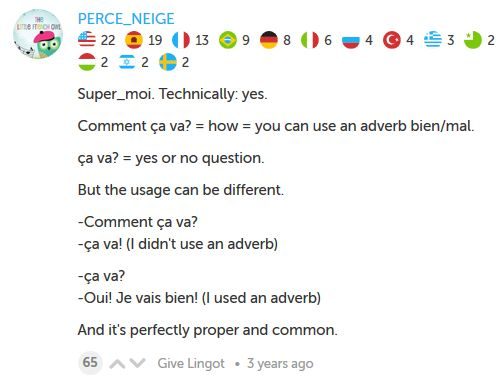
\includegraphics[scale = 0.5]{images/cava.jpg}
\end{center}

\subsubsection{Liaisons}

In a liaison, an otherwise silent ending consonant is pushed to the next word, where it's pronounced as part of the first syllable. Like elisions, this prevents consecutive vowel sounds. Liaisons are possible whenever a silent ending consonant is followed by a word beginning in a vowel sound, but some liaisons are mandatory and others are forbidden.  Here are some mandatory liaisons, along with approximate pronunciations:

\begin{itemize}
  \item  Articles and adjectives with nouns. For example, un homme ("uh-nohm") \\ mon orange ("mohn-norahnge"), or deux hommes ("duh-zohm").
  \item  Pronouns and verbs. For example, nous allons ("noo-zalohn") or est-il ("ay-teel").
  \item  Single-syllable adverbs and prepositions. For instance, très utile ("tray-zuteel") or chez elle ("shay-zell").
\end{itemize}

Liaisons that are forbidden:

\begin{itemize}
  \item  Before and after et ("and").
  \item  After singular nouns (including proper nouns and names).
  \item  After inversions (which you'll learn in "Questions").
  \item  Before an aspirated H (e.g. héros - "hero").
  \item  After a nasal sound, except that un, on, and en do liaise.
\end{itemize}

Note that some consonants take on a different sound in liaisons, and it's important to pronounce these correctly when speaking.\footnote{Liaison rules vary among speakers, particularly across dialects, and fewer liaisons tend to appear in casual and slow speech. Note that the slow mode in Duo listening exercises does not include liaisons.}

\begin{center}\begin{tabular}{|c|c|c|}
\hline
\textbf{Original Consonant} & \textbf{Resulting Liaison Sound} & \textbf{Example}                    \\ \hline
-s, -x, -z                  & Z                                & des hommes ("day-zohm")             \\ \hline
-d                          & T                                & un grand arbre ("uhn-grahn-tarbre") \\ \hline
-f                          & V                                & neuf ans ("nuh-vahn")               \\ \hline
\end{tabular}\end{center}

\subsubsection{Encha{\^i}nement}

In encha{\^i}nements, ending consonant sounds are pushed onto the next word if it begins in a vowel. This is essentially the same as a liaison, except that the consonant sound wasn't silent beforehand. For instance:

\begin{itemize}
  \item  elle est is pronounced like "eh-lay".
  \item  mange une pomme is pronounced like "mahn-jun-pom".
\end{itemize}

\subsubsection{The Impersonal Expression Il Y A}

Impersonal expressions are phrases where there isn't a real subject. For instance, in the phrase "It is snowing" (Il neige), "it" doesn't refer to anything. It's a dummy subject that exists just to maintain the sentence structure.  One of the most common impersonal expressions is il y a, which is an idiom for "there is" or "there are".

\begin{itemize}
  \item  Il y a une fille ici. \\ There is a girl here.
  \item  Il y a un serpent dans ma botte ! \\ There's a snake in my boot!
\end{itemize}

\subsubsection{Vocabulary}

\begin{center}\begin{tabular}{l|l||l|l}
\textbf{French} & \textbf{English} & \textbf{French} & \textbf{English} \\ \hline
oui & yes & {\c c}a va & how are you? \\
non & no & comment {\c c}a va & how are you? \\
s'il vous pla{\^i}t & please & {\c C}a va bien & I am well. \\
merci & thank you & pardon & pardon me \\
merci beaucoup & thank you very much & d{\' e}sol{\' e} & sorry \\
bonjour & hello & Bienvenue! & Welcome! \\
bonsoir & good evening & {\`A} bient{\^o}t! & See you soon! \\
salut & bye & {\`A} plus tard! & See you later! \\
au revoir & goodbye & {\`A} demain! & See you tomorrow! \\
bonne nuit & good night & D'accord & Okay \\
\end{tabular}\end{center}

\begin{itemize}
  \item  Oui, je suis d{\' e}sol{\' e}. \\ Yes, I am sorry.
\end{itemize}


\pagebreak
\subsection{Food}

\subsubsection{The Partitive Article}

The partitive article is used for unspecified amounts of uncountable nouns. In English, it can translate to "some", but it's often just omitted. Remember that du is a contraction of de + le and that partitives can elide.

\begin{center}\begin{tabular}{|c|c|c|}
\hline
\textbf{Gender} & \textbf{Partitive Article} & \textbf{Example}                               \\ \hline
Masculine       & du                         & Je mange du poisson. — I am eating fish.       \\ \hline
Feminine        & de la                      & Je mange de la viande. — I am eating meat.     \\ \hline
Elided Masc.    & de l'                      & Je mange de l'ananas. — I am eating pineapple. \\ \hline
Elided Fem.     & de l'                      & Je bois de l'eau. — I am drinking water.       \\ \hline
\end{tabular}\end{center}

Nouns almost never appear without articles in French, so articles must be repeated in serial lists.  For example,

\begin{itemize}
  \item  Il cuisine du poisson et de la viande \\ He cooks fish and meat.
\end{itemize}

\subsubsection{Count Noun, Mass Noun, or Both?}

\textbf{Count nouns} are discrete and can be counted, like un livre ("a book"). They can be modified by definite and indefinite articles, but not partitive articles.

\begin{itemize}
  \item  Je lis un livre. \\ I am reading a book.
  \item  Nous avons les livres. \\ We have the books.
\end{itemize}

\textbf{Mass nouns} like lait ("milk") are uncountable, and they can be modified by definite and partitive articles, but not indefinite articles.

\begin{itemize}
  \item  Je bois du lait. \\ I am drinking [some] milk.
  \item  Je bois le lait. \\ I am drinking the milk.
\end{itemize}

However, many nouns can behave as both count nouns and mass nouns. This is true for most edible things. For instance, consider poisson ("fish") or vin ("wine"):

\begin{itemize}
  \item  Count noun: Le poisson est rouge. \\ The fish is red.
  \item  Mass noun: Je mange du poisson. \\ I eat [some] fish.
  \item  Count noun: Le vin est blanc. \\ The wine is white.
  \item  Mass noun: Je bois du vin rouge ou blanc. \\ I drink red or white wine.
\end{itemize}

Note that some mass nouns can be pluralized in English when they refer to multiple types of the noun, but this usage isn't found in French. For instance, "the fishes" refers to multiple species of fish, while les poissons just refers to multiple fish.

\subsubsection{Omitted Articles}

When an article is missing in an English sentence, it must be added to the French translation. The definite article can be used to fill this void in three situations:

\begin{itemize}
  \item  Almost anywhere one would use "the" in English (i.e. when referring to specific things).
  \item  Before the subject of a sentence to state general truths about it.
  \item  Before the direct object of a verb of appreciation (like aimer) to express like/dislike.
\end{itemize}

If any of the above is true, then use the definite article. Otherwise, use the indefinite or partitive, depending on whether or not the noun is countable.

\begin{itemize}
  \item  I like wine, but I am drinking milk. \\ J'aime le vin, mais je bois du lait.
\end{itemize}

Both articles are missing in the English version of this example. Aimer expresses fondness for wine, so le vin should be used there. However, boire is not a verb of appreciation, so the partitive du should be used on the uncountable lait.

\begin{itemize}
  \item  Cats are animals. \\ Les chats sont des animaux.
\end{itemize}

This is a general truth about cats, but (2) above can only apply to subjects, so only chats takes a definite article here. Animaux are countable, so use the plural indefinite des.

\begin{itemize}
  \item  He likes to eat meat. \\ Il aime manger de la viande.
\end{itemize}

This is a tricky example because the meat is the direct object of manger, not aimer. Thus, (3) does not apply and viande cannot take a definite article.  Also, the French definite article can be ambiguous when translating from French to English. It can often refer to both a specific noun and the general sense of a noun.

\begin{itemize}
  \item  Les chats sont des animaux. \\ Cats are animals. / The cats are animals.
\end{itemize}
    
\subsubsection{De + Definite Article}

De plus a definite article can also have other meanings. De means "of" or "from", so this can also indicate possession or association with a definite noun.

\begin{itemize}
  \item  La copie du livre. \\ The copy of the book.
  \item  Les copies des livres. \\ The copies of the books.
  \item  L'enfant de la femme. \\ The woman's child.
\end{itemize}

\subsubsection{Vocabulary}

\begin{center}\begin{tabular}{l|l||l|l}
\textbf{French} & \textbf{English} & \textbf{French} & \textbf{English} \\ \hline
boivent & to drink & \Blue{le repas} & meal \\
mangent & to eat & \Red{la boisson} & beverage \\
cuisine & to cook & \Blue{le th{\'e}} & tea \\
\Blue{le sandwich} & sandwich & \Red{la cr{\^e}pe} & crepe \\
\Red{la tomate} & tomato & \Blue{le beurre} & butter \\
\Red{la soupe} & soup & \Blue{le fromage} & cheese \\
\Red{la fraise} & strawberry & \Blue{le poisson} & fish \\
\Red{la viande} & beef & \Blue{le bonbon} & candy \\
\Red{la baguette} & baguette & \Red{la banane} & banana \\
\Blue{le oignon} & onion & \Blue{le sel} & salt \\
l'eau & water & \Blue{le poivre} & pepper \\
l'{\oe}uf & egg & \Blue{le sucre} & sugar \\
l'alcool & alcohol & \Blue{le poulet} & chicken \\
\Red{la salade} & salad & \Blue{le porc} & pork \\
\Blue{le riz} & rice & \Blue{le g{\^a}teau} & cake \\
\Red{la bi{\`e}re} & beer & \Blue{le citron} & lemon \\
\Blue{le lait} & milk & \Blue{le chocolat} & chocolate \\
\Blue{le pain} & bread & \Blue{le b{\oe}uf} & beef \\
\Blue{le vin} & wine & \Blue{le raisin} & grape \\
\Blue{le caf{\'e}} & coffee & \Blue{le jus} & juice \\
avec & with \\
\end{tabular}\end{center}

\begin{itemize}
  \item  Je bois de la bi{\`e}re. \\ I drink beer.
  \item  Les hommes mangent du fromage. \\ The men drink beer.
  \item  Nous avons du sucre. \\ We have sugar.
\end{itemize}


\pagebreak
\subsection{Animals}

\subsubsection{Noun Genders}

One of the most difficult aspects of learning French is memorizing noun genders. However, by spending some time now memorizing the following patterns, you may be able to guess most nouns' genders and save yourself a lot of trouble in the future.  Some nouns, like l'élève ("the student"), have the same spelling and meaning in both forms. Other nouns have the same spelling, but have different meanings. Un tour is a tour, while une tour is a tower. There are also nouns that only have one possible gender. Even a baby girl is un bébé, for instance. Many masculine nouns can be changed to a feminine form simply by adding an -e to the end. Your male friend is un ami and your female friend is une amie.  Some genders depend on a noun's classification. For instance, languages, days of the week, months, seasons, metals, colors, and measurements are mostly masculine.  Otherwise, memorizing word endings is the best way to guess genders. We'll learn these ending patterns in four steps:

\begin{enumerate}
  \item  Nouns ending in -e tend to be feminine. All others, especially nouns ending in consonants, tend to be masculine. This is true for over 70\% of all nouns.
  \item  Nouns that have the endings -ion and -son tend to be feminine, even though they end in consonants.
  \item  Nouns with these endings are usually masculine, although they end in -e:
    \begin{itemize}
      \item  -tre, -ble, -cle (think "treble clef")
      \item  -one, -ème, -ège (think "OMG")
      \item  -age, -isme
    \end{itemize}
  \item  Watch out for these complications:
    \begin{itemize}
      \item  -é is masculine, but -té is feminine. \\ le résumé (masc) — the resumé \\ la liberté (fem) — the liberty
      \item  -de is masculine, but -ade, -nde, and -ude are feminine. \\ le guide — the guide \\ la parade — the parade
      \item  -ste and -me tend to be masculine, but there are dozens of exceptions. Words for people ending in -ste are often gender-neutral, e.g. le/la cycliste.
      \item  -eur is masculine for most professions or technical terms, but it's feminine for some emotions and abstract things. \\ le chauffeur — the driver \\ la peur — the fear
    \end{itemize}
\end{enumerate}

That's it! Memorize these, and you'll be able to guess most noun genders.

\subsubsection{Feminine Animals}

In French, female animal nouns are generally formed as follows by taking the last consonant, doubling it, and adding a mute -e to the end.

\begin{itemize}
  \item  un chat $\quad\Rightarrow\quad$ une chatte
  \item  un chien $\quad\Rightarrow\quad$ une chienne
\end{itemize}

Of course, there are many exceptions. For example:

\begin{itemize}
  \item  un ours $\quad\Rightarrow\quad$ une ourse (not une oursse)
  \item  un cheval $\quad\Rightarrow\quad$ une jument (not une chevalle)
\end{itemize}

\subsubsection{Vocabulary}

\begin{center}\begin{tabular}{l|l||l|l}
\textbf{French} & \textbf{English} & \textbf{French} & \textbf{English} \\ \hline
\Purple{cheval} & horse & \Blue{le singe} & monkey \\
\Purple{chien} & dog & \Purple{requin} & shark \\
\Blue{l'animal} & animal & \Red{l'abeille} & bee \\
\Blue{l'oiseau} & bird & \Purple{serpent} & snake \\
\Purple{canard} & duck & \Blue{l'araign{\'e}e} & spider \\
\Purple{chat} & cat & \Red{la souris} & mouse \\
\Purple{l'{\'e}l{\'e}phant} & elephant & \Blue{le papillon} & butterfly \\
\Purple{ours} & bear & \Blue{l'insecte} & insect \\
\Red{la tortue} & turtle & \Red{la fourmi} & ant \\
\Purple{lion} & lion & \Red{la baleine} & whale \\
\Red{la vache} & cow & \Blue{le dauphin} & dolphin \\
\Purple{cochon} & pig & \Blue{le loup}, \Red{la louve} & wolf \\
\Red{la mouche} & [house]fly & \Purple{lapin} & rabbit \\
\Blue{le tigre} & tiger & \Red{la poule} & hen \\
\end{tabular}\end{center}


\pagebreak
\subsection{Adjectives}

Unlike English adjectives, French adjectives must agree in number and gender with the nouns that they modify. A black dog is un chien noir, but a black dress is une robe noire. Also, remember that some adjectives have the same masculine and feminine form, especially those ending in a silent -e (e.g. riche).  When used with pronouns, adjectives agree with the noun that has been replaced. This is particularly tricky with the formal vous: to a singular man, you would say vous êtes beau, but to plural women, you would say vous êtes belles.

\subsubsection{Adjective Placement}

In French, most adjectives appear after the nouns they modify. For instance, le chat noir. However, some adjectives precede the noun. You can remember these types of nouns using the mnemonic \Purple{BANGS}.

\begin{itemize}
  \item  \Purple{B} is for beauty. Une belle femme $\quad\Rightarrow\quad$ A beautiful woman
  \item  \Purple{A} is for age. Une jeune fille $\quad\Rightarrow\quad$ A young girl
  \item  \Purple{N} is for number.\footnote{This can also be for rank: Le premier mot — The first word} Deux hommes $\quad\Rightarrow\quad$ Two men
  \item  \Purple{G} is for good or bad. Un bon garçon $\quad\Rightarrow\quad$ A good boy
  \item  \Purple{S} is for size. Un gros chat $\quad\Rightarrow\quad$ A fat cat
\end{itemize}

All determiner adjectives (e.g. possessives, interrogatives, and demonstratives) appear before the noun, e.g. mon livre ("my book") and ce cochon ("that pig"). You will learn these later.

\subsubsection{Figurative Adjectives}

A few adjectives can come both before and after the noun depending on their meaning. The most common example is grand, which is a BANGS adjective for everything but people. For people, it comes before a noun when it means "important" and after the noun when it means "tall". For instance, Napoleon was un grand homme ("a great man"), but not un homme grand ("a tall man").  Usually, figurative meanings will precede the noun, while literal meanings will follow the noun.

\begin{itemize}
  \item  un pauvre homme $\quad\Rightarrow\quad$ a pitiful man
  \item  un homme pauvre $\quad\Rightarrow\quad$ a poor man
  \item  un certain nombre $\quad\Rightarrow\quad$ a certain (particular) number
  \item  une victoire certaine $\quad\Rightarrow\quad$ a certain (guaranteed) victory
  \item  ma propre voiture $\quad\Rightarrow\quad$ my own car
  \item  ma voiture propre $\quad\Rightarrow\quad$ my clean car
  \item  un cher ami $\quad\Rightarrow\quad$ a dear friend
  \item  une montre chère $\quad\Rightarrow\quad$ an expensive watch
\end{itemize}

\subsubsection{Euphony}

As you have already learned, elisions, contractions, liaisons, and enchaînements are all designed to prevent consecutive vowel sounds (which is called hiatus). This quest for harmonious sounds is called euphony and is an essential feature of French. It has, however, created some unexpected rules.  For instance, the masculine beau ("beautiful") changes to bel if its noun begins with a vowel sound. A beautiful man is un bel homme. The other two common changes are vieux to vieil ("old") and nouveau to nouvel ("new").  Note that this doesn't occur to feminine adjectives because they usually end in silent vowels.
    
\subsubsection{Vocabulary}

\begin{center}\begin{tabular}{l|l||l|l}
\textbf{French} & \textbf{English} & \textbf{French} & \textbf{English} \\ \hline
froid & cold & grand & large \\
chaud & hot & jeune & young \\
nouveau & new & joil & pretty \\
petit & small \\
\end{tabular}\end{center}


\pagebreak
\subsection{Plurals}

Most plural forms of nouns and adjectives can be formed by appending an -s to the singular, but remember that this -s is usually silent.

\begin{itemize}
  \item  Le chat noir $\quad\Rightarrow\quad$ The black cat $\quad\Rightarrow\quad$ Les chats noirs $\quad\Rightarrow\quad$ The black cats
  \item  Un chat noir $\quad\Rightarrow\quad$ A black cat $\quad\Rightarrow\quad$ Des chats noirs $\quad\Rightarrow\quad$ (Some) black cats
\end{itemize}

Note: If the noun is preceded by an adjective, des becomes de.

\begin{itemize}
  \item  Un petit chat $\quad\Rightarrow\quad$ A little cat $\quad\Rightarrow\quad$ De petits chats
\end{itemize}

Articles must agree with the nouns they modify, so plural nouns require either les or des. This is a great way to tell if a noun is plural. If you hear les or des (which sound similar to "lay" and "day"), then the noun is plural. If not, it's probably singular.  Remember that verbs change conjugation to agree with their subjects in both grammatical person and number.

\begin{center}\begin{tabular}{|r|c|l|}
\hline
\textbf{Subject}    & \textbf{{\^E}tre ("to be")} & \textbf{Parler ("to speak")} \\ \hline
\textbf{je}         & suis                    & parle                        \\ \hline
\textbf{tu}         & es                      & parles                       \\ \hline
\textbf{il/elle/on} & est                     & parle                        \\ \hline
\textbf{nous}       & sommes                  & parlons                      \\ \hline
\textbf{vous}       & {\^e}tes                & parlez                       \\ \hline
\textbf{ils/elles}  & sont                    & parlent                      \\ \hline
\end{tabular}\end{center}

\subsubsection{Punctuation}

There are no quotation marks in French. Instead, the French use guillemets (\guillemotleft \guillemotright). Exclamation marks (!), question marks (?), colons (:), semicolons (;) and guillemets need to have a space on either side.

\begin{itemize}
  \item  Incorrect: ``{\c C}a va?''
  \item  Correct: \guillemotleft~{\c C}a va ? \guillemotright
\end{itemize}

When writing numbers in French, commas are decimal points, while spaces mark thousands places.

\begin{itemize}
  \item  Incorrect: 1,235.8
  \item  Correct: 1 235,8
\end{itemize}



\pagebreak
\chead{Chapter 2}
\section{Chapter 2}

\subsection{To Be and To Have}

{\^E}tre and avoir are the most common verbs in French. Like many common verbs, they have irregular conjugations.

\begin{center}\begin{tabular}{|r|c|l|}
\hline
\textbf{Subject}    & \textbf{{\^E}tre ("to be")} & \textbf{Avoir ("to have")} \\ \hline
\textbf{je}         & (je)suis                & (j')ai                     \\ \hline
\textbf{tu}         & es                      & as                         \\ \hline
\textbf{il/elle/on} & est                     & a                          \\ \hline
\textbf{nous}       & sommes                  & avons                      \\ \hline
\textbf{vous}       & {\^e}tes                & avez                       \\ \hline
\textbf{ils/elles}  & sont                    & ont                        \\ \hline
\end{tabular}\end{center}

There should be a liaison between ils or elles and ont ("il-zon" or "elle-zon"). The "z" sound is essential here to differentiate between "they are" and "they have", so be sure to emphasize it.  These two verbs are very important because they can act as auxiliary verbs in French, but they differ from their English equivalents. In "Basics 2", you learned that "I write" and "I am writing" both translate to j'{\'e}cris, not je suis {\'e}cris. This is because {\^e}tre cannot be used as an auxiliary in a simple tense. It can only be used in compound tenses, which you will learn in the "Pass{\'e} Compos{\'e}" unit.  Another important distinction is that avoir means "to have" in the sense of "to possess", but not "to consume" or "to experience". Other verbs must be used for these meanings.

\subsubsection{C'est or Il Est?}

When describing people and things with {\^e}tre in French, you usually can't use a personal subject pronoun like elle. Instead, you must use the impersonal pronoun ce, which can also mean "this" or "that". Note that ce is invariable, so it can never be ces sont.

\begin{center}\begin{tabular}{|c|c|c|}
\hline
                  & \textbf{Impersonal Subject Pronoun} & \textbf{Personal Subject Pronoun} \\ \hline
\textbf{Singular} & c'est                               & il/elle est                       \\ \hline
\textbf{Plural}   & ce sont                             & ils/elles sont                    \\ \hline
\end{tabular}\end{center}

These pronouns aren't interchangeable. The basic rule is that you must use ce when {\^e}tre is followed by any determiner---for instance, an article or a possessive adjective. Note that c'est should be used for singulars and ce sont should be used for plurals.

\begin{itemize}
  \item  C'est un homme.---He's a man. / This is a man. / That is a man.
  \item  Ce sont des chats.---They're cats. / These are cats. / Those are cats.
  \item  C'est mon chien.---It's my dog. / This is my dog. / That's my dog.
\end{itemize}

If an adjective, adverb, or both appear after {\^e}tre, then use the personal pronoun.

\begin{itemize}
  \item  Elle est belle.---She is beautiful. (Or "It is beautiful.")
  \item  Il est tr{\`e}s fort.---He is very strong. (Or "It is very strong.")
\end{itemize}

As you know, nouns generally need determiners, but one important exception is that professions, nationalities, and religions can act as adjectives after {\^e}tre. \\ 
This is optional; you can also choose to treat them as nouns.

\begin{itemize}
  \item  He is a doctor.---Il est m{\'e}decin. / C'est un m{\'e}decin.
\end{itemize}

However, c'est should be used when using an adjective to make a general comment about (but not describe) a thing or situation. In this case, use the masculine singular form of the adjective.

\begin{itemize}
  \item  C'est normal ?---Is this normal?
  \item  Non, c'est {\'e}trange.---No, this is strange.
\end{itemize}

\subsubsection{Idioms with Avoir}

One of the most common idioms in French is the use of the verb avoir in certain places where English would use the verb "to be". This is especially common for states or conditions that a person may experience.

\begin{itemize}
  \item  Elle a chaud.---She is hot. (Or "She feels hot.")
  \item  Il a froid.---He is cold.
  \item  Elle a deux ans.---She is two years old.
  \item  J'ai peur !---I am afraid!
\end{itemize}

French tends to use the verb faire ("to do") idiomatically for general conditions like weather.\footnote{Note that il fait is an impersonal expression with no real subject, just like il y a from "Common Phrases".}

\begin{itemize}
  \item  Il fait chaud.---It is hot (outside).
  \item  Il fait froid.---It is cold.
  \item  Il fait nuit.---It is nighttime.
\end{itemize}

\begin{itemize}
  \item  C'est de la soupe. \\ This is soup
  \item  C'est la soupe. \\ This is the soup
  \item  C'est du vin. \\ That is wine.
\end{itemize}


\pagebreak
\subsection{Clothing}

\subsubsection{Idiomatic Plurals}

English has a number of idiomatic plural-only nouns that have to be translated carefully. These are not just nouns that are invariable with number (like "deer"), but rather nouns that cannot refer to a singular thing at all.  For instance, "the pants" can only be plural in English, but the corresponding le pantalon is singular in French. A single pair of pants is not les pantalons, which refers to multiple pairs of pants. Similarly, when translating le pantalon back to English, you can say "the pants" or "a pair of pants", but "a pant" is not correct. This also applies to un jean ("a pair of jeans").  Un v{\^e}tement refers to a single article of clothing, and it's incorrect to translate it as "clothes", which is plural and refers to a collection of clothing. This would have to be des v{\^e}tements.

\subsubsection{Diacritics}

The \textbf{acute accent} ({\'e}) only appears on E and produces a pure [e] that isn't found in English. To make this sound, say the word ``clich{\'e}'', but hold your tongue perfectly still on the last vowel to avoid making a diphthong sound.

The \textbf{grave accent} ({\`e}) can appear on A/E/U, though it only changes the sound for E (to [ɛ], which is the E in "lemon"). Otherwise, it distinguishes homophones like a (a conjugated form of avoir) and {\`a} (a preposition).

The \textbf{cedilla} ({\c c}) softens a normally hard C sound to the soft C in ``cent''. Otherwise, a C followed by an A, O, or U has a hard sound like the C in ``car''.

The \textbf{circumflex} ({\^e}) usually means that an S used to follow the vowel in Old French or Latin. (The same is true of the acute accent.) For instance, {\^i}le was once ``isle''.

The \textbf{trema} ({\"e}) indicates that two adjacent vowels must be pronounced separately, like in No{\"e}l ("Christmas") and ma{\"i}s ("corn").

\subsubsection{Nasal Vowels}

There are four nasal vowels in French. Try to learn these sounds by listening to native speakers.

\begin{center}\begin{tabular}{|c|c|c|}
\hline
\textbf{IPA} & \textbf{Letter Sequence} & \textbf{Examples}       \\ \hline
/œ̃/         & un/um                    & un/parfum               \\ \hline
/ɛ̃/         & in/im/yn/ym              & vin/pain/syndicat/sympa \\ \hline
/ɑ̃/         & an/am/en/em              & dans/chambre/en/emploi  \\ \hline
/ɔ̃/         & on/om                    & mon/ombre               \\ \hline
\end{tabular}\end{center}

These aren't always nasalized. If there's a double M or N, or if they are followed by any vowel, then the vowel should have an oral sound instead. For instance, un is nasal, but une is not. Also, vin is nasal, but vinaigre is not.

\subsubsection{Vocabulary}

\begin{center}\begin{tabular}{l|l||l|l}
\textbf{French} & \textbf{English} & \textbf{French} & \textbf{English} \\ \hline
\Blue{le sac} & bag & \Blue{le manteau} & coat  \\ 
\Red{la poche} & pocket & \Red{la vest} & jacket  \\ 
\Red{la ceinture} & belt & \Blue{le chapeau} & hat  \\ 
\Blue{le v{\^e}tement, les v{\^e}tements} & clothes & \Red{la chaussette} & sock  \\ 
\Blue{le pantalon, les pantalons} & pair of pants, pants & \Blue{le jean, les jeans} & pair of jeans, jeans \\
\Red{la chaussure} & shoe & \Blue{le parapluie} & umbrella  \\ 
\Red{la chemise} & shirt & \Blue{le gant} & glove  \\ 
\Red{la jupe} & skirt & \Red{la casquette} & cap  \\ 
\Blue{le botte} & boot  & \Red{l'{\'e}charpe} & scarf \\ 
\Blue{le costume} & suit & \Red{la cravate} & necktie \\ 
\Blue{le portefeuille} & wallet \\
\end{tabular}\end{center}


\pagebreak
\subsection{Colors}

Colors can be both nouns and adjectives. As nouns, colors are usually masculine (e.g. \guillemotleft~ Le rose \guillemotright~ = ``The pink'').

As adjectives, they agree with the nouns they modify except in two cases. First, colors derived from nouns (e.g. fruits, flowers, or gems) tend to be invariable with gender and number. Orange ("orange") and marron ("brown") are the most common examples.

\begin{itemize}
  \item  La jupe orange \\ The orange skirt
  \item  Les jupes orange \\ The orange skirts
  \item  Les chiens marron \\ The brown dogs
\end{itemize}

Second, in compound adjectives (les adjectifs composés) made up of two adjectives, both adjectives remain in their masculine singular forms.

\begin{itemize}
  \item  Sa couleur est vert pomme. \\ Its color is apple-green.
  \item  J'aime les robes rose clair. \\ I like light-pink dresses.
\end{itemize}

Most colors that end in -e in their masculine forms are invariable with gender.

\begin{itemize}
  \item  Un chien rouge \\ A red dog
  \item  Une jupe rouge \\ A red skirt
\end{itemize}

\huge

%http://www.rapidtables.com/web/color/RGB_Color.htm

\begin{center}\begin{tabular}{l|l||l|l}
\textbf{French} & \textbf{English} & \textbf{French} & \textbf{English} \\ \hline
\Blue{le couleur} & color & \textcolor[RGB]{255,0,0}{rouge} & \textcolor[RGB]{255,0,0}{red} \\
blanc & white &  \textcolor[RGB]{255,165,0}{orange} & \textcolor[RGB]{255,165,0}{orange} \\ 
noir & black & \textcolor[RGB]{255,255,0}{jaune} & \textcolor[RGB]{255,255,0}{yellow} \\ 
\textcolor[RGB]{128,128,128}{gris} & \textcolor[RGB]{128,128,128}{gray} & \textcolor[RGB]{0,128,0}{verte} & \textcolor[RGB]{0,128,0}{green} \\ 
\textcolor[RGB]{255,192,203}{rose} & \textcolor[RGB]{255,192,203}{pink} & \textcolor[RGB]{0,0,255}{bleu} & \textcolor[RGB]{0,0,255}{blue} \\ 
\textcolor[RGB]{165,42,42}{marron} & \textcolor[RGB]{165,42,42}{brown} & \textcolor[RGB]{128,0,128}{violet} & \textcolor[RGB]{128,0,128}{purple} \\ 
\end{tabular}\end{center}

\normalsize

\begin{itemize}
  \item  La fille a une jolie robe rose. \\ The girl has a pretty pink dress.
\end{itemize}


\pagebreak
\subsection{Possessives}

In English, possessive adjectives (e.g. ``his'') match the owner. However, in French, they match the thing being owned.  Consider the example of ``her lion''. The French translation is \guillemotleft~ son lion \guillemotright , because lion is masculine and both the lion and the woman are singular. Note that if we hear just \guillemotleft~ son lion \guillemotright , we can't tell if the lion is owned by a man or woman. It's ambiguous without more context. If two people own a lion, then it is  \guillemotleft~ leur lion \guillemotright .

Possessives have different forms that agree with four things: the number of owners, the number of things owned, the gender of the thing owned, and the grammatical person of the owner (e.g. "his" versus "my").  For one owner, the possessive adjectives are:

\begin{center}\begin{tabular}{|c|c|c|c|c|}
\hline
\textbf{Person} & \textbf{English} & \textbf{Masculine Singular} & \textbf{Feminine Singular} & \textbf{Plural} \\ \hline
\textbf{1st}    & my               & mon                         & ma                         & mes             \\ \hline
\textbf{2nd}    & your (singular)  & ton                         & ta                         & tes             \\ \hline
\textbf{3rd}    & his/her/its      & son                         & sa                         & ses             \\ \hline
\end{tabular}\end{center}

For multiple owners, genders don't matter:

\begin{center}\begin{tabular}{|c|c|c|c|}
\hline
\textbf{Person} & \textbf{English} & \textbf{Singular Owned} & \textbf{Plural Owned} \\ \hline
\textbf{1st}    & our              & notre                   & nos                   \\ \hline
\textbf{2nd}    & your (plural)    & votre                   & vos                   \\ \hline
\textbf{3rd}    & their            & leur                    & leurs                 \\ \hline
\end{tabular}\end{center}

The plural second-person possessive adjectives, votre and vos, should be used when addressing someone formally with vous.

\begin{center}\begin{tabular}{|c|l|l|}
\hline
\textbf{Owner}   & \multicolumn{1}{c|}{\textbf{Singular Owned}} & \multicolumn{1}{c|}{\textbf{Plural}} \\ \hline
\textbf{My}      & Mon ami---My friend                          & Mes tigres---My tigers               \\ \hline
\textbf{Your}    & Ton abeille---Your bee                       & Tes lions---Your lions               \\ \hline
\textbf{His/Her} & Son oiseau---His/her bird                    & Ses chiens---His/her dogs            \\ \hline
\textbf{Our}     & Notre bi{\`e}re---Our beer                   & Nos pommes---Our apples              \\ \hline
\textbf{Your}    & Votre sel---Your salt                        & Vos citrons---Your lemons            \\ \hline
\textbf{Their}   & Leur fromage---Their cheese                  & Leurs fromages---Their cheeses       \\ \hline
\end{tabular}\end{center}

\subsubsection{Euphony in Possessives}

For the sake of euphony, all singular feminine possessives switch to their masculine forms when followed by a vowel sound.

\begin{center}\begin{tabular}{|c|c|c|c|}
\hline
\textbf{Person} & \textbf{Masculine} & \textbf{Feminine} & \textbf{Feminine + Vowel Sound} \\ \hline
1st             & mon chat           & ma robe           & mon eau                         \\ \hline
2nd             & ton chat           & ta robe           & ton eau                         \\ \hline
3rd             & son chat           & sa robe           & son eau                         \\ \hline
\end{tabular}\end{center}

\subsubsection{Femme and Fille}

Femme can mean "woman" or "wife" and fille can mean "girl" or "daughter" depending on the context. For example, when femme and fille are preceded by a possessive adjective, then they translate to "wife" and "daughter", respectively.

\begin{itemize}
  \item  Une fille et une femme sont dans le restaurant \\ A girl and a woman are in the restaurant. (Not: "A daughter and a wife are in the restaurant.")
  \item  Ma fille \\ My daughter. (Not: "My girl".)
  \item  Ta femme \\ Your wife. (Not: "Your woman".)
\end{itemize}


\pagebreak
\subsection{Present Tense 1}

As you learned in ``Basics 1'', verbs like parler conjugate to agree with their subjects. Parler itself is an infinitive, which is a verb's base form. It consists of a root (parl-) and an ending (-er). The ending can dictate how the verb should be conjugated. In this case, almost all verbs ending in -er are regular verbs in the 1st Group that share the same conjugation pattern. To conjugate another 1st Group verb, affix the ending to that verb's root.

\begin{itemize}
  \item  Aimer ("to love"): j'aime, tu aimes, nous aimons, etc.
  \item  Marcher ("to walk"): je marche, tu marches, nous marchons, etc. 
\end{itemize}

Every verb belongs to one of three groups:

\begin{itemize}
  \item  The \textbf{1st Group} includes regular -er verbs and includes 80\% of all verbs.\footnote{Aller (``to go'') is the only fully irregular verb in Group 1, but a handful of others are slightly irregular.}
  \item  The \textbf{2nd Group} includes regular -ir verbs like finir ('to finish").
  \item  The \textbf{3rd Group} includes all irregular verbs. This includes many common verbs like {\^e}tre and avoir as well as a handful of less common conjugation patterns.
\end{itemize}

\begin{center}\begin{tabular}{|r|l|l|l|}
\hline
\textbf{Subject} & \textbf{G1: parler} & \textbf{G2: finir} & \textbf{G3: dormir} \\ \hline
je               & parl\Blue{e}               & fini\Red{s}              & dor\textbf{s}                \\ \hline
tu               & parl\Blue{es}              & fini\Red{s}              & dor\textbf{s}                \\ \hline
il/elle/on       & parl\Blue{e}               & fini\Red{t}              & dor\textbf{t}                \\ \hline
nous             & parl\Blue{ons}             & fini\Red{ssons}          & dor\textbf{mons}             \\ \hline
vous             & parl\Blue{ez}              & fini\Red{ssez}           & dor\textbf{mez}              \\ \hline
ils/elles        & parl\Blue{ent}             & fini\Red{ssent}          & dor\textbf{ment}             \\ \hline
\end{tabular}\end{center}

\textbf{Spelling-changing} verbs end in -ger (e.g. manger) or -cer (e.g. lancer, ``to throw'') and change slightly in the nous form, as well as any other form whose ending begins with an A or O. These verbs take a form like nous mangeons or nous lan{\c c}ons.

\textbf{Stem-changing} verbs have different roots in their nous and vous forms. For instance, most forms of appeler (``to call'') have two L's (e.g. j'appelle), but the N/V forms are nous appelons and vous appelez. 

\subsubsection{Semi-Auxiliary Verbs}

The only true auxiliary verbs in French are {\^e}tre and avoir, but there are a number of semi-auxiliary verbs in French that can be used with other verbs to express ability, necessity, desire, and so on. They are used in \textbf{double-verb} constructions where the first verb (the semi-auxiliary) is conjugated and the second is not.

\begin{itemize}
  \item  Je veux lire. \\ I want to read.
  \item  Il aime manger. \\ He likes to eat.
\end{itemize}

Modal verbs are the English equivalents of semi-auxiliaries.  For instance, ``can'', translates to either savoir or pouvoir. When ``can'' indicates knowledge, use savoir.  When ``can'' indicates permission or ability (apart from knowledge), use pouvoir.

\begin{itemize}
  \item  Je sais lire et {\'e}crire. \\ I know how to read and write.
  \item  Il sait parler allemand. \\ He knows how to speak German.
  \item  Il peut manger. \\ He can (or "may") eat.
  \item  Il peut parler allemand. \\ He is allowed to speak German.
\end{itemize}

One of the most important semi-auxiliary verbs is aller, which is used to express the near future (futur proche), just like the English verb ``going to''. 

\begin{itemize}
  \item  Je vais manger. \\ I am going to eat.
  \item  Vous allez lire le livre. \\ You are going to read the book.
\end{itemize}

Note that in verb constructions beginning with non-auxiliary verbs, the verbs must be separated by a preposition.

\begin{itemize}
  \item  Nous vivons pour manger. \\ We live to eat.
\end{itemize}

\subsubsection{Impersonal Expressions}

A few defective impersonal verbs can only be used in impersonal statements and must be conjugated as third-person singular with il. Remember that il is a dummy subject and does not refer to a person.  Falloir means ``to be necessary'', and it often takes the form il faut + infinitive.  Il faut can also be used transitively with a noun to indicate that it is needed.

\begin{itemize}
  \item  Il faut manger. \\ It is necessary to eat. / One must eat.
  \item  Il faut choisir. \\ It is necessary to choose. / One must choose.
  \item  Il faut du pain. \\ (Some) bread is needed.
\end{itemize}

\subsubsection{Confusing Verbs}

Used transitively, savoir and connaître both mean ``to know'', but in different ways. Savoir implies understanding of subjects, things, or skills, while connaître indicates familiarity with people, animals, places, things, or situations.

\begin{itemize}
  \item  Je sais les mots. \\ I know the words.
  \item  Je connais le garçon. \\ I know the boy.
\end{itemize}

Attendre means ``to await'', which is why it does not need a preposition.

\begin{itemize}
  \item  Il attend son ami. \\ He is awaiting (or "waiting for") his frien
\end{itemize}

\subsubsection{One Each}

The indefinite article doesn't always refer to just one thing. Sometimes, it can mean one thing each. Consider these examples:

\begin{itemize}
  \item  Ils ont un manteau \\ They have one coat / They each have one coat
  \item  Ils ont des manteaux \\ They have some coats / They each have some coats
\end{itemize}

\subsubsection{Vocabulary}

\begin{center}\begin{tabular}{l|l||l|l}
\textbf{French} & \textbf{English} & \textbf{French} & \textbf{English} \\ \hline
lire & to read & faire & to make \\ 
{\'e}crivent & to write & vais & going to \\ 
parler & to talk & acheter & to buy \\ 
aimer & to like & aider & to help \\ 
vouloir & to want & appeller & to call \\ 
boivent & to drink & apporter & to bring \\
comprender & to understand & apprender & to learn \\ 
pouvoir & to be able to & attender & to wait for \\ 
doivent & must & chercher & to look for \\ 
adorer & to love &  savent & to know \\
faut & need to & conna\^{\i}re & to know (people) \\
commander & to be in charge \\
\end{tabular}\end{center}


\pagebreak
\subsubsection{Demonstratives 1}

Demonstrative adjectives (this, that, these, and those) modify nouns so they refer to something or someone specific. They can be used in place of articles. Like other adjectives, they must agree with the nouns they modify.

\begin{center}\begin{tabular}{|c|c|c|}
\hline
\textbf{Gender}    & \textbf{Singular} & \textbf{Plural} \\ \hline
\textbf{Masculine} & ce/cet            & ces             \\ \hline
\textbf{Feminine}  & cette             & ces             \\ \hline
\end{tabular}\end{center}

The singular masculine ce becomes cet in front of a vowel sound for euphony.

\begin{itemize}
  \item  Ce livre est rouge. \\ That book is red.
  \item  Cet arbre est grand. \\ That tree is big.
  \item  Cette pomme est rouge. \\ That apple is red.
  \item  Ces livres et ces pommes sont rouges. \\ Those books and those apples are red.
\end{itemize}

Ce can mean either ``this'' or ``that''. It's ambiguous between the two. To specify, use the suffix -ci (``here'') or -l{\`a} (``there'') on the modified noun.

\begin{itemize}
  \item  Ce livre-ci est rouge. \\ This book is red.
  \item  Ces chats-l{\`a} sont noirs. \\ Those cats are black. 
\end{itemize}

French learners often confuse the demonstrative adjective ce with the pronoun ce (from ``{\^E}tre-Avoir''). Discerning between them is easy, however: an adjective must modify a noun, while a pronoun can stand alone as a subject or object. Compare:

\begin{itemize}
  \item  Adjective: Ces hommes sont mes amis. \\ These men are my friends.
  \item  Pronoun: Ce sont mes amis. \\ They are my friends. 
\end{itemize}

In the first example, ces is an adjective that modifies hommes, but in the second, ce is a subject pronoun.

\subsubsection{{\c C}a}

The indefinite demonstrative pronoun {\c c}a refers to an unnamed concept or thing. When it's used as an object, it usually translates to ``this'' or ``that''.

\begin{itemize}
  \item  Tu manges {\c c}a. \\ You are eating this.
  \item  Je veux {\c c}a. \\ I want that.
\end{itemize}

{\c C}a can also be used as a subject, in which case it can also mean ``it''.

\begin{itemize}
  \item  {\c C}a sent bon. \\ It smells good.
  \item  {\c C}a semble simple. \\ This seems simple.
\end{itemize}

\subsubsection{{\c C}a or Ce?}

A simple rule of thumb to follow is that ce should be used with {\^e}tre, including in the double-verb constructions pouvoir {\^e}tre and devoir {\^e}tre.

\begin{itemize}
  \item  C’est un très bon vin ! \\ This is a really good wine!
  \item  Ce sont des garçons. \\ They are boys.
  \item  Ce peut être triste en hiver. \\ It can be sad in winter.
  \item  Ce doit être ton fils. \\ It must be your son.
\end{itemize}

{\c C}a should be used with all other verbs.

\begin{itemize}
  \item  {\c C}a va bien. \\ It's going well.
  \item  {\c C}a dure un jour. \\ That lasts a day.
  \item  {\c C}a m'intéresse beaucoup. \\ That interests me a lot.
\end{itemize}

However, when an object pronoun comes before {\^e}tre, then you must use {\c c}a, not ce. This is relatively rare.

\begin{itemize}
  \item  {\c C}a m'est {\'e}gal. \\ It's all the same to me.
\end{itemize}

Also, note that {\c c}a is informal and is usually replaced by cela (``that'') or ceci (``this'') in writing.


\pagebreak
\subsection{Conjunctions 1}

Conjunctions function by hooking up words, phrases, and clauses. This unit focuses on coordinating conjunctions, which link two or more similar elements in a sentence. For instance, \guillemotleft et \guillemotright may be used to link two nouns together.

\begin{itemize}
  \item  Je mange une pomme et une orange. \\ I am eating an apple and an orange.
  \item  Elle a un chien et un chat. \\ She has a dog and a cat.
\end{itemize}

It may also link two adjectives or even two clauses.

\begin{itemize}
  \item  La robe est grande et jolie. \\ The dress is big and pretty.
  \item  Le chat est noir et le chien est blanc. \\ The cat is black and the dog is white.
\end{itemize}

For the most part, French coordinating conjunctions behave very similarly to their English counterparts.

\begin{center}\begin{tabular}{|c|c|c|c|}
\hline
\textbf{Conjunction} & \textbf{English} & \textbf{Exemple} & \textbf{Example}                             \\ \hline
et                   & and              & Elle a un chien et un chat. & She has a dog and a cat.          \\ \hline
mais                 & but              & Mais pas maintenant. & But not now.                             \\ \hline
ou                   & or               & Oui ou non ? & Yes or no?                                       \\ \hline
comme                & as/like          & Je suis comme ça. & I am like that.                             \\ \hline
donc                 & so/thus          & Il est jeune, donc il est petit. & He is young, so he is small. \\ \hline
car                  & because          & Jelis, car j'aime ce livre. & I read because I like this book.  \\ \hline
\end{tabular}\end{center}

The conjunction \guillemotleft car \guillemotright means ``because'', and it's usually reserved for writing. The subordinating conjunction \guillemotleft parce que  \guillemotright is preferred in speech; you'll learn this in \textit{Conjunctions 2}.

\begin{itemize}
  \item  Comme vous savez. \\ As you know.
  \item  Elle mange du pain \Blue{quand} elle veut. \\ She eats bread \Blue{when} she wants.
  \item  Je lis, \Blue{car} j'aime le livre. \\ I read \Blue{because} I like the book.
\end{itemize}


\pagebreak
\subsection{Questions}
\subsubsection{Inversions}

The most formal way of asking a question is to use an \textbf{inversion}, where the verb appears before its pronoun and the two are connected by a hyphen.

\begin{itemize}
  \item  Boit-il ? \\ Does he drink? / Is he drinking? / He drinks?
  \item  Boivent-ils du lait ? \\ Do they drink milk? / Are they drinking milk? / They drink milk?
\end{itemize}

However, if the subject of the sentence is a noun, then the noun should appear before the verb, although a pronoun still needs to appear afterwards.

\begin{itemize}
  \item  Le lait est-il froid ? \\ Is the milk cold?
  \item  Les chats sont-ils noirs ? \\ Are the cats black?
\end{itemize}

If the verb ends in a vowel, the letter T must be inserted after the verb for euphony. This T is chained onto the pronoun and is meaningless.

\begin{itemize}
  \item  A-t-il un chien ? \\ Does he have a dog?
  \item  Parle-t-elle anglais ? \\ Does she speak English?
\end{itemize}

Inverted forms still obey other grammar rules, like those for \guillemotleft~ il est \guillemotright versus \guillemotleft~ c'est \guillemotright . However, the pronoun in an inversion cannot elide.

\begin{itemize}
  \item  Est-ce un probl{\`e}me ? \\ Is it a problem?
  \item  Est-elle m{\'e}decin ? \\ Is she a doctor?
  \item  Puis-je aider les enfants ? \\ Can I help the children?
\end{itemize}

\subsubsection{Est-ce Que}

\textbf{Est-ce que} (pronounced like ``essk'') can be added in front of a statement to turn it into a question. Remember that \guillemotleft~ que \guillemotright elides in front of vowel sounds.

\begin{itemize}
  \item  \textbf{Est-ce qu'il} boit ? \\ Does he drink? / Is he drinking?
  \item  \textbf{Est-ce que} c'est un probl{\`e}me ? \\ Is it a problem?
  \item  \textbf{Est-ce qu'il} a un chien ? \\ Does he have a dog?
\end{itemize}

\subsubsection{Intonation}

In informal speech, one of the most common ways to ask a question is simply to raise your intonation at the end of a statement, like you'd do in English.

\begin{itemize}
  \item  Il boit ? \\ Is he drinking?
  \item  Il pleut ? \\ Is it raining?
\end{itemize}


\pagebreak
\subsection{Interrogatives}

An \textbf{interrogative} word introduces a question. French has interrogative adjectives, pronouns, and adverbs.

\subsubsection{Interrogative Adjectives}

French has one interrogative adjective with four forms. It translates to ``which'' or ``what'' depending on the context.

\begin{center}\begin{tabular}{|l|l|l|}
\hline
\textbf{Gender}    & \textbf{Singular} & \textbf{Plural} \\ \hline
\textbf{Masculine} & quel              & quels           \\ \hline
\textbf{Feminine}  & quelle            & quelles         \\ \hline
\end{tabular}\end{center}

An interrogative adjective cannot stand alone. It must modify (and agree with) a noun, and that noun must either be adjacent to it or separated by a form of {\^e}tre.

\begin{itemize}
  \item  Quelle fille ? \\ Which girl?
  \item  Quel est le probl{\`e}me ? \\ What is the problem?
\end{itemize}

Quel is also an exclamatory adjective in statements.

\begin{itemize}
  \item  Quelle chance ! \\ What luck!
  \item  Quel grand gar{\c c}on il est ! \\ What a tall boy he is!
\end{itemize}

\subsubsection{Interrogative Pronouns}

Unlike an adjective, an interrogative pronoun can stand alone. For instance, the interrogative pronoun lequel can replace quel + noun. Note that it agrees with the noun it replaces.

\begin{center}\begin{tabular}{|c|c|}
\hline
\textbf{Quel Form}                            & \textbf{Lequel Form}                     \\ \hline
Quel cheval ?---Which horse?                  & Lequel?---Which one?                     \\ \hline
Quels hommes mangent ?---Which men eat?       & Lesquels mangent ?---Which ones eat?     \\ \hline
Quelle robe est rose ?---Which dress is pink? & Laquelle est rose ?---Which one is pink? \\ \hline
Quelles lettres ?---Which letters?            & Lesquelles ?---Which ones?               \\ \hline
\end{tabular}\end{center}

The most common interrogative pronouns are \guillemotleft qui \guillemotright (for people) and \guillemotleft que \guillemotright (for everything else). However, the construction changes based on a number of factors. Qui is the only pronoun that can start a question by itself, but both qui and que can be used with inversion.

\begin{itemize}
  \item  Qui parle ? \\ Who is speaking?
  \item  Qui es-tu ? \\ Who are you?
  \item  Que fait-il ? \\ What is he making?
\end{itemize}

Both can also use est-ce, but est-ce que (which you learned above) can only be used in a question with {\^e}tre or when the pronoun is the object (``what'' or ``whom''). When it is the subject, est-ce qui must be used.

\begin{itemize}
  \item  Qui est-ce qui parle ? \\ Who's speaking? (subj.)
  \item  Qu'est-ce qui se passe ? \\ What is going on? (subj.)
  \item  Qui est-ce que tu appelles ? \\ Whom are you calling? (obj.)
  \item  Qu'est-ce que c'est ? \\ What is it? (question with {\^e}tre)
\end{itemize}

After prepositions and at the end of questions, \guillemotleft que \guillemotright becomes \guillemotleft quoi \guillemotright .

\begin{itemize}
  \item  Le probl{\`e}me est quoi ? \\ What's the problem?
  \item  {\`A} quoi pensez-vous ? \\ What are you thinking about?
\end{itemize}

Qui and que can be very confusing because they can also be relative pronouns. Que can also be a subordinating conjunction. You will learn these uses later.

\subsubsection{Interrogative Adverbs}

A number of interrogative adverbs can be used to request information

\begin{itemize}
  \item  Pourquoi (``why''): Pourquoi manges-tu du pain ?---Why are you eating bread?
  \item  Comment (``how''): Comment allez-vous ?---How are you?
  \item  Quand (``when''): Quand est-ce que tu vas manger ?---When are you going to eat?
  \item  Combien (``how many/much''): Combien d'eau ?---How much water?
  \item  O{\`u} (``where''): O{\`u} suis-je ?---Where am I?
\end{itemize}

Note that when these adverbs are used with intonation-based questions, they can appear at the beginning or the end of the sentence (except pourquoi).

\begin{itemize}
  \item  Tu vas comment ? \\ How are you?
  \item  Vous {\^e}tes d'o{\`u} ? \\ Where are you from?
\end{itemize}


\pagebreak
\subsection{Present Tense 2}

As you learned in ``Verbs Present 1'', Group 3 verbs are considered irregular, but some sparse patterns do exist among the -ir and -er verbs in this group.

\begin{center}\begin{tabular}{|l|l|l|l|l|l|}
\hline
\textbf{Subject} & \textbf{G1 parler} & \textbf{G2 finir} & \textbf{G3 dormir} & \textbf{G3 ouvrir} & \textbf{G3 vendre} \\ \hline
je               & parl\textbf{e}              & fini\textbf{s}             & dor\textbf{s}               & ouvr\textbf{e}              & vend\textbf{s}              \\ \hline
tu               & parl\textbf{es}             & fini\textbf{s}             & dor\textbf{s}               & ouvr\textbf{es}             & vend\textbf{s}              \\ \hline
il/elle/on       & parl\textbf{e}              & fini\textbf{t}             & dor\textbf{t}               & ouvr\textbf{e}              & vend               \\ \hline
nous             & parl\textbf{ons}            & fini\textbf{ssons}         & dor\textbf{mons}            & ouvr\textbf{ons}            & vend\textbf{ons}            \\ \hline
vous             & parl\textbf{ez}             & fini\textbf{ssez}          & dor\textbf{mez}             & ouvr\textbf{ez}             & vend\textbf{ez}             \\ \hline
ils/elles        & parl\textbf{ent}            & fini\textbf{ssent}         & dor\textbf{ment}            & ouvr\textbf{ent}            & vend\textbf{ent         }   \\ \hline
\end{tabular}\end{center}

Among the G3 -ir verbs, some conjugate like dormir, while verbs like ouvrir conjugate as though they're -er verbs. Note that singular conjugations of dormir drop the last letter of the root. Also, while some -re verbs (such as attendre, entendre, and perdre) conjugate like vendre, dozens of other conjugation patterns exist, so it's best to memorize each verb's conjugation individually.

\subsubsection{Transitive and Intransitive Verbs}

Sentences can have grammatical objects, which are nouns that are affected by a verb. There are two types of objects: \textbf{direct objects}, which are nouns acted upon, and \textbf{indirect objects}, which are nouns that are indirectly affected by the action.  In the example ``Ben threw the ball at him'', ``Ben'' is the subject, ``the ball'' is the direct object, and ``him'' is the indirect object. You can usually recognize indirect objects in English by looking for a preposition after a verb. Identifying objects is important, especially in French.  Verbs can be \textbf{transitive}, \textbf{intransitive}, or both. Transitive verbs can have direct objects, while intransitive verbs cannot. However, both types of verbs can have indirect objects.

\begin{itemize}
  \item  Transitive: Je lance une chaussure. \\ I throw a shoe.
  \item  Intransitive: Je parle {\`a} Jacques. \\ I am speaking to Jacques.
\end{itemize}

\textit{Parler} is an interesting example because it's intransitive for everything but language names.

\begin{itemize}
  \item  Transitive: Je parle anglais. \\ I speak English.
\end{itemize}

French verbs can be tricky for Anglophones because some transitive verbs in French have intransitive English translations and vice versa. Pay attention to this.

\begin{itemize}
  \item  Transitive: Le chat regarde le chien. \\ Intransitive: The cat is looking at the dog.
  \item  Intransitive: Il t{\'e}l{\'e}phone {\`a} son ami. \\ Transitive: He is calling his friend.
\end{itemize}

\subsubsection{Stative Verbs in English}

Unlike dynamic verbs, which describe actions and processes, stative verbs describe states of being, physical and mental states, possession, sensations, and so on. The most common stative verb is ``to be''. Here are some other common examples:

\begin{itemize}
  \item  Possessing: belong, get, have, own, possess
  \item  Feeling: hate, like, love, need, want
  \item  Sensing: feel, hear, see, smell, taste
  \item  Thinking: believe, know, recognize, think, understand
\end{itemize}

The most important detail about stative verbs is that they can't be used in continuous tenses in English.

\begin{itemize}
  \item  C'est mon fils. \\ He is my son. (Not ``is being''.)
  \item  Je veux une pomme. \\ I want an apple. (Not ``am wanting''.)
  \item  Elle aime son chien. \\  She loves her dog. (Not ``is loving''.) 
  \item  On a deux amis. \\ We have two friends. (Only cannibals ``are having'' their friends.)
\end{itemize}

You may have noticed that some verbs can be both stative and dynamic based on context. For instance:

\begin{itemize}
  \item  ``To have'' can be dynamic when it means ``to consume''.
  \item  ``To feel'' is stative, but ``to feel sick" or "to feel better'' are dynamic.
  \item  ``To be'' can be dynamic when it means ``to act''.
\end{itemize}

Pay attention to this nuance when translating into English. This problem rarely occurs when translating to French because it lacks continuous tenses. 

\subsubsection{Impersonal Expressions}

A number of other impersonal verbs have to do with weather.

\begin{itemize}
  \item  Pleuvoir (``to rain''): Il pleut. \\ It is raining.
  \item  Neiger (``to snow''): Il neige. \\ It is snowing.
  \item  Faire chaud (``to be warm''): Il fait chaud aujourd'hui. \\ It is warm today.
\end{itemize}

Chaud can be replaced with a number of other adjectives, like froid (``cold'') or humide (``humid'').

\subsubsection{Confusing Verbs}

Like their English counterparts, voir (``to see'') and regarder (``to watch'') differ based on the subject's intention. If the subject is actively watching or looking for something, use regarder. Otherwise, use voir.

\begin{itemize}
  \item  Le chat regarde le poisson. \\ The cat is watching the fish.
  \item  Elle peut voir la ville. \\ She can see the city.
\end{itemize}

\subsubsection{Vocabulary}

\begin{center}\begin{tabular}{l|l||l|l}
\textbf{French} & \textbf{English} & \textbf{French} & \textbf{English} \\ \hline
respecter & to respect & porter & to carry \\ 
contenir & to contain & poser & to set down \\ 
couper & to cut & poss{\`e}der & to own \\ 
courir & to run & prendre & to take \\ 
cuire & to cook & proposer & to suggest \\ 
dire & to say & saisir & to grab \\ 
donner & to give & souhaiter & to wish \\ 
entrer & to enter & suivre & to follow \\ 
finir & to finish & terminer & to finish \\ 
gagner & to win & tenir & to hold \\ 
int{\'e}resser & to interest & trouver & to find \\ 
lancer & to throw & vendre & to sell \\ 
laver & to wash & voir & to see \\ 
marcher & to walk & vivre & to live \\ 
m{\'e}riter & to deserve & ajouter & to add \\ 
mettre & to put & am{\'e}liorer & to improve \\ 
montrer & to show & concerner & to concern \\ 
cacher & to hide & casser & to break \\ 
motiver & to motivate & devenir & to become \\ 
neiger & to snow & dormir & to sleep \\ 
pleuter & to rain & entendre & to hear \\ 
ourvir & to open & regarder & to watch \\ 
perdre & to lose \\
\end{tabular}\end{center}

\begin{itemize}
%  \item  J'agis. \\ I am taking action.
%  \item  J'ai mal agi. \\ I have acted poorly.
  \item  O{\`u} vivez-vous? \\ Where do you live?
  \item  Le livre concerne une femme. \\ The book has to do with a woman.
\end{itemize}


\pagebreak
\subsection{Adjectives 2}

When multiple adjectives modify a noun, they should come before or after the noun based on the same rules as if they were the only adjective. This means that adjectives may straddle the noun if one is a BANGS adjective.

\begin{itemize}
  \item  La grande robe rouge \\ The big red dress
  \item  Une jeune fille fran{\c c}aise \\ A young French girl
\end{itemize}

When arranging multiple adjectives on the same side, concrete adjectives should usually be placed closer to the noun than abstract ones.

\begin{itemize}
  \item  J'ai un joli petit chat gris. \\ I have a lovely little grey cat.
  \item  J'ai un chat blanc courageux. \\ I have a brave white cat.
\end{itemize}

You can add conjunctions and adverbs to break up multiple adjectives.

\begin{itemize}
  \item  J'ai un chapeau blanc et bleu. \\ I have a white and blue hat.
  \item  L'homme fort et s{\'e}rieux \\ The strong and serious man.
  \item  Voici mon premier petit chat blanc et courageux. \\ Here is my first small white and brave cat.
  \item  J'adore mon propre tout petit chat blanc tr{\`e}s doux. \\ I love my own tiny white and very soft cat.
\end{itemize}

When there are multiple nouns being described by one adjective, that adjective takes the masculine plural by default.

\begin{itemize}
  \item  Un garçon et une fille italiens \\ An Italian boy and girl
  \item  J'ai une chemise et un manteau simples. \\ I have a simple shirt and coat.
\end{itemize}

However, if the nouns are all feminine, then they can take the feminine plural.

\begin{itemize}
  \item  La robe et la jupe vertes \\ The green dress and skirt
\end{itemize}

\pagebreak
\subsubsection{Grand or Gros?}

Grand and gros can both mean "big", but they're only partly interchangeable.  Grand tends to be used for:

\begin{itemize}
  \item  General size: La grande robe---The big dress
  \item  Height: L'enfant est grand.---The child is tall/big.
  \item  Area: La ville est grande.---The city is big.
  \item  Figurative size: La grande richesse---The great wealth
  \item  Importance: Un grand homme---A great man
\end{itemize}

Gros tends to be used for:

\begin{itemize}
  \item  Thickness or volume: Une grosse boîte de petits-pois---A big can of peas
  \item  Fatness: Un gros chat---A fat cat
  \item  Things that are round: Une grosse pomme---A big apple
  \item  Seriousness: Un gros probl{\`e}me---A big (serious) problem
\end{itemize}

\subsubsection{Faux Amis}

Many English and French words look alike and share meanings. This is because English is heavily influenced by French and Latin. However, there are faux amis (``false friends'') that look similar but do not have the same meaning. For instance, gros looks like ``gross'', but their meanings are not the same. Be careful before assuming a French word's meaning based on its English lookalike.

\pagebreak
\subsubsection{Vocabulary}

\begin{center}\begin{tabular}{l|l||l|l}
\textbf{French} & \textbf{English} & \textbf{French} & \textbf{English} \\ \hline
bon & good (BANGS) & gros & fat \\ 
m{\^e}me & same & b{\^e}te & stupid \\ 
premi{\`e}re & first & {\'e}norme & enormous \\ 
long & long & dr{\^o}le & funny \\ 
bien & good & m{\'e}chant & vicious \\ 
dernier & shirt & laid & ugly \\ 
beau & beautiful & japonais & Japanese \\ 
g{\'e}nial & brilliant & sombre & dark (colored) \\ 
belle & beautiful (BANGS) & anglaise & English \\ 
simple & simple & europ{\'e}ens & European \\ 
fran{\c c}aise & french & italien & Italian \\ 
second & second & chinois & Chinese \\ 
mauvais & bad (BANGS) & espagnol & Spanish \\ 
difficile & difficult & africaine & African \\ 
nombreux & numerous & sympa & friendly \\ 
impossible & impossible & am{\'e}ricain & American \\ 
deuxi{\`e}me & second (BANGS) & s{\'e}rieux & serious \\ 
troisi{\`e}me & third (BANGS) & pr{\^e}t & ready \\ 
diff{\'e}rent & different & sec & dry \\ 
important & important & allemand & German \\ 
clair & light (colored) & gentil & gentle \\ 
fort & strong & seul & only (BANGS) \\ 
large & big & propre & clean \\ 
pauvre & poor & sale & dirty \\ 
dur & hard & l{\'e}g{\`e}r & light[weight] \\ 
grosse & large & joli & pretty \\ 
\end{tabular}\end{center}


\pagebreak
\subsection{Pronouns}

\subsubsection{On}

\guillemotleft On \guillemotright is a versatile and ubiquitous French indefinite subject pronoun. Francophones usually say on to refer to ``us'', ``them'', or one or more unidentified persons. \guillemotleft On \guillemotright is always masculine and third-person singular, which is why conjugation charts often list il/elle/on together.

\begin{itemize}
  \item  On mange. \\ We are eating.
  \item  On est seul. \\ We are alone.
\end{itemize}

\guillemotleft On \guillemotright can also be used more formally in the passive voice or for general statements, much like the English ``one''.

\begin{itemize}
  \item  On doit dormir assez. \\ One must sleep adequately.
\end{itemize}

\subsubsection{Direct Objects}

\begin{center}\begin{tabular}{|c|c|}
\hline
\textbf{English}           & \textbf{Direct Object} \\ \hline
me                         & me                     \\ \hline
you (sing.)                & te                     \\ \hline
him                        & le                     \\ \hline
her                        & la                     \\ \hline
us                         & nous                   \\ \hline
you(plur. or formal sing.) & vous                   \\ \hline
them                       & les                    \\ \hline
\end{tabular}\end{center}

Direct object pronouns usually come before their verbs.

\begin{itemize}
  \item  L'enfant me voit. \\ The child sees me.
  \item  Le lion le mange. \\ The lion eats it (or "him"!).
  \item  Vous nous aimez. \\ You love us.
  \item  Je t'aime. \\ I love you.
\end{itemize}

Me/te/le/la elide, so make sure you notice them when they hide in the first syllable of a verb.

\begin{itemize}
  \item  Elle m'attend. \\ She is waiting for me.
  \item  L'enfant l'appelle. \\ The child calls to him/her.
\end{itemize}

Le and les only contract when they're articles, not when they're object pronouns.

\begin{itemize}
  \item  Je suis en train de le faire. (Not du faire) \\ I am in the process of doing it.
\end{itemize}

\subsubsection{En Replaces De + Noun}

The adverbial pronoun \guillemotleft en \guillemotright can be used to replace objects introduced by de. For instance, it can replace a partitive article + noun.

\begin{itemize}
  \item  Avez-vous de l'argent ? \\ Do you have some money?
  \item  Oui, j'en ai. \\ Yes, I have some.
\end{itemize}

\guillemotleft En \guillemotright may replace nouns or pronouns in verb constructions that use de, like parler de (``to talk about'').

\begin{itemize}
  \item  Marc parle de son fr{\`e}re ? \\ Is Marc talking about his brother?
  \item  Oui, il en parle. \\ Yep, he's talking about him.
\end{itemize}

Nouns in adverbs of quantity can also be replaced with \guillemotleft en \guillemotright .

\begin{itemize}
  \item  Achetez-vous beaucoup de livres ? \\ Are you buying a lot of books?
  \item  Oui, j'en ach{\`e}te beaucoup. \\ Yes, I am buying a lot [of them].
\end{itemize}

\subsubsection{Y Can Refer to a Place}

The adverbial pronoun \guillemotleft y \guillemotright can refer to a previously mentioned or implied place, in which case it's usually translated as ``there''.  In English, ``there'' may be omitted, but the same is not true of \guillemotleft y \guillemotright in French. \guillemotleft Je vais \guillemotright is not a complete sentence without \guillemotleft y \guillemotright .

\begin{itemize}
  \item  Allez-vous au restaurant ? \\ Are you going to the restaurant?
  \item  Oui, j'y vais. \\ Yes, I'm going there.
\end{itemize}

\subsubsection{The Relative Pronouns Que and Qui}

\textbf{Relative pronouns} introduce relative clauses, which are subordinate clauses that elaborate upon a previously mentioned noun (the antecedent). Use \guillemotleft que \guillemotright when the relative pronoun is the direct object (``whom'' in English) and use \guillemotleft qui \guillemotright when it is the subject (``who'' in English).

\begin{itemize}
  \item  C'est l'homme que je connais. \\ He's the man whom (or ``that'') I know.
  \item  La fille qui lit un menu. \\ The girl who (or ``that'') reads a menu.
\end{itemize}

If you have trouble figuring out whether to use \guillemotleft qui \guillemotright or \guillemotleft que \guillemotright , try rephrasing the sentence without the relative pronoun. Use \guillemotleft qui \guillemotright if the antecedent is the subject; otherwise, use \guillemotleft que \guillemotright .

\begin{itemize}
  \item  Subject: La fille qui lit un menu. $\Rightarrow$ La fille lit un menu.
  \item  Object: C'est l'homme que je connais. $\Rightarrow$ Je connais l'homme.
\end{itemize}

\subsubsection{The Reflexive Pronoun Se}

A \textbf{reflexive pronoun} like \guillemotleft se \guillemotright can be used to indicate that a verb acts upon the subject. \guillemotleft Se \guillemotright is used with all third-person subjects, regardless of gender and number.

\begin{itemize}
  \item  Il s'aime. \\ He loves himself.
  \item  Il s'appelle comment ? \\ What's his name? (Lit, "He calls himself what?")
  \item  Elle se demande pourquoi. \\ She wonders why. (Lit, "She asks herself why.")
\end{itemize}

When \guillemotleft se \guillemotright refers to a plural subject, it can also be reciprocal or mutual (``each other'').

\begin{itemize}
  \item  Ils s'aiment. \\ They love each other.
  \item  Les filles se parlent. \\ The girls speak to each other.
  \item  On se parle quand ? \\ When do we speak to each other?
  \item  On se voit bient{\^o}t. \\ We will see each other soon.
\end{itemize}

Certain pronouns can be added to the end of the sentence to differentiate between reflexive and reciprocal uses if necessary.

\begin{itemize}
  \item  Ils s'aiment eux-m{\^e}mes. \\ They love themselves.
  \item  Elles s'aiment elles-m{\^e}mes. \\ They love themselves.
  \item  Ils s'aiment l'un l'autre. \\ They love each other.
  \item  Elles s'aiment les unes les autres. \\ They love one another.
\end{itemize}

\begin{itemize}
  \item  {\c C}a se peut. \\ It can be done.
  \item  Qu'est-ce que tu as ? \\ What have you got?
  \item  Je sais o{\`u} c'est. \\ I know where it is.
  \item  Je veux boire quelque chose. \\ I want to drink something.
\end{itemize}

\pagebreak
\chead{Chapter 3}
\section{Chapter 3}

\subsection{Possessive Pronouns}

\subsubsection{Personal Pronouns in the Nominative Case}

A pronoun is a word that represents a noun, like ``er'' does for ``der Mann''" In the nominative case, the personal pronouns are simply the grammatical persons you already know: ``ich'', ``du'', ``er/sie/es'', ``wir'', ``ihr'', ``sie'', and ``Sie''.

\subsubsection{Demonstrative Pronouns in the Nominative Case}

The demonstrative pronouns in English are: this, that, these, and those. In German, the demonstrative pronouns in the nominative case are the same as the definite articles. That means, ``der'', ``die'', and ``das" can also mean ``that (one)'' or ``this (one)'' depending on the gender of the respective noun, and ``die'' can mean ``these'' or ``those''. For example, if you talk about a certain dog, you could say ``Der ist schwarz'' (that one is black).

\begin{center}\begin{tabular}{c|c}
  mein/meine & unser/unsere \\
	\hline
	dein/deine & euer/euere \\
	\hline
	sein/seine/ihr/ihre & seins \\
\end{tabular}\end{center}

\vspace{0.5in}

\begin{center}
  
\includegraphics[bb=0 0 640 480]{images/Wassermelone.jpg}
\end{center}


\pagebreak
\subsection{Nominative Pronouns}

\begin{center}\begin{tabular}{l|l}
  \textbf{Deutsch} & \textbf{English} \\
	\hline
	beide/beides/beiden & both \\
	dieser/diese/dies & these \\
	jeder/jede/jedes & each one \\
	manche & some \\
	viele & a lot of \\
	alle & everybody \\
	alles & everything \\
	viel & a lot \\
	niemand & nobody \\
	jemand & anyone \\
	etwas & some \\
	paar & a few \\
\end{tabular}\end{center}

It's ``beide'' when it's `both' in the nominative and accusative without an article like the sentence above, ``Beide m{\"o}gen Kaffee'' or ``Ich mag beide''.

It's ``beiden'' in the dative case when there's no article as in ``Mit beiden H{\"a}nden'' or ``Gib beiden Menschen Kaffee'', etc.

It's also ``beiden'' when it follow the plural definite article as in ``Die beiden sind groß''. It's like that in all cases: Nominative: die beiden Accusative: die beiden Dative: den beiden Genitive: der beiden

And then there's ``beides''

``beide'' is used in the plural, for countable objects:

``Soll ich Mama oder Papa holen?'' - ``Beide sollen kommen!'' ``Das Radio und das Grammophon standen im Freien, beide wurden nass vom Regen.''

``beides'' is used in the singular, for uncountable objects or abstract objects:

``Magst du Ketchup oder Mayo auf die Pommes?'' - ``Beides muss drauf!'' ``Was machst du lieber: Geschirr sp{\"u}len oder W{\"a}sche b{\"u}geln?'' - ``Das ist beides {\"a}tzend!''

\pagebreak
\subsection{Negatives}

\begin{center}\begin{tabular}{l|l}
  \textbf{Deutsch} & \textbf{English} \\
	\hline
	nicht & not (temporary condition) \\
	kein & not (permanent condition) \\
	keine & not one (feminine) \\
	keinen & not any \\
	keiner & nobody \\
	\Red{Die Steuer} & tax \\
	nie & never \\
	niemals & never ever (i.e. with emphasis) \\
	nichts & nothing \\
\end{tabular}\end{center}


\pagebreak
\subsection{Adverbs 1}

\begin{center}\begin{tabular}{l|l}
  \textbf{Deutsch} & \textbf{English} \\
	\hline
	auch & too \\
	zu & too \\
	so & so \\
	gern & like \\
	gerne & like (either form is accepted) \\
	wirklich & really \\
	noch & still \\
	noch eine & another \\
	nur & only \\
	schon & already \\
	immer & always \\
	genug & enough \\
	in Ordnung & alright \\
	zusammen & together \\
	dran & turn (as in ``It is my turn'') \\
	vielleicht & might [be] \\
	wieder & again \\
	alleine & alone \\
\end{tabular}\end{center}

Examples:
\begin{itemize}
  \item  Ich lerne gern.
  \item  Ich trinke gerne Wein.
\end{itemize}


\pagebreak
\subsection{Places 1}

\begin{center}\begin{tabular}{l|l}
  \textbf{Deutsch} & \textbf{English} \\
	\hline
	das Geb{\"a}ude & building \\
	das Haus (die H{\"a}user) & house (houses) \\
	\Blue{der Markt} & market \\
	\Red{die Schule (die Schulen)} & school (schools) \\
	\Blue{der G{\"a}rten} & garden \\
	\Red{die Ecke} & corner \\
	\Blue{der Bahnhof (die Bahnh{\"o}fe)} & train station (train stations) \\
	das Restaurant (die Restaurants) & restaurant (restaurants) \\
	\Red{die Bibliothek} & library \\
	das Schloss (die Schlosses) & castle (castles) \\
	\Red{die Bank} & bank \\
	bauen & to build \\
	das Land (die L{\"a}nder) & country (countries) \\
	das Hotel & hotel \\
	\Red{die Stra{\ss}e} & street \\
	\Red{die Stadt} & city \\
	das Dorf (die D{\"o}rfer) & village (villages) \\
	\Red{die Br{\"u}cke} & bridge \\
	\Blue{der Park (die Parks)} & park (parks) [noun] \\
	das Zimmer (die Zimmer) & room (rooms) [as in bedroom, living room, etc.] \\
\end{tabular}\end{center}


\pagebreak
\subsection{Stuff}

German is well known for its very long words that can be made up on the go by concatenating existing words. In this skill you will learn one very simple and commonly used way of forming compounds: adding ``-zeug'' (``stuff'') to existing words.

\begin{center}\begin{tabular}{l|l}
  \textbf{Deutsch} & \textbf{English} \\
	\hline
	das Zeug & stuff \\
	das Fahrzeug (die Fahrzeuge) & vehicle (vehicles) \\
	das Flugzeug (die Flugzeuge) & airplane (airplanes) \\
	das Feuerzeug (die Feuerzeuge) & lighter (lighters) \\
	das Spielzeug (die Spielzeuge) & toy (toys) \\
	das Werkzeug (die Werkzeuge) & tool (tools) \\
\end{tabular}\end{center}


\pagebreak
\subsection{Accusative Pronouns}

\subsubsection{Personal Pronouns in the Accusative Case}

Aside from the nominative case, most of the German pronouns are declined in each of the four cases. Like in English, when the subject becomes the object, the pronoun changes. For instance, ``ich'' changes to ``mich'' (accusative object) as in ``Ich sehe mich'' (I see me).

In the accusative case of the third person pronouns, only the masculine gender shows the change, thus neither the feminine ``sie'' nor the neuter ``es'' change. For example, ``Er/Sie/Es mag ihn/sie/es'' (He/She/It likes him/her/it).

\begin{center}\begin{tabular}{l|l}
  \textbf{Nominative} & \textbf{Accusative} \\
	\hline
	ich (I) & mich (me) \\
	du (you, singular informal) & dich (you, singular informal) \\
	\Blue{er (he)} & \Blue{ihn (him)} \\
	sie (she) & sie (her) \\
	es (it) & es (it) \\
	wir (we) & uns (us) \\
	ihr (you, plural informal) & euch (you, plural informal) \\
	sie (they) & sie (them) \\
	Sie (you, formal) & Sie (you, formal) \\
\end{tabular}\end{center}

\subsubsection{Demonstrative Pronouns in the Accusative Case}

Similarly, only the masculine gender shows the change in the demonstrative pronouns: ``der'' (for ``that one'') changes to ``den'', but ``die'' and ``das'' (for ``that one'') remain the same.

The demonstrative pronouns in the accusative case are thus: ``den'' = that one (masculine), ``die'' = that one (feminine), ``das'' = that one (neuter), and for the plural, ``die'' = ``these''. Take this example: ``Er isst den'' is ``He is eating that one (masculine)''; ``Er isst die'' and ``Er isst das'' are both ``He is eating that one'', but for the other two genders.


\pagebreak
\subsection{Household 1}

\begin{center}\begin{tabular}{l|l}
  \textbf{Deutsch} & \textbf{English} \\
	\hline
	{\"o}ffnen & to open \\
	\Red{die Wand} & wall \\
	\Red{die Decke} & blanket (or ceiling) \\
	das Fenster & window \\
	\Red{die T{\"u}r} & door \\
	\Blue{der Zaun (die Z{\"a}une)} & fence \\
	\Red{die Treppe} & staircase \\
	\Red{die Wohnung} & apartment \\
	das Dach & roof \\
	\Blue{der Balkon} & balcony \\
	\Blue{der Schl{\"u}ssel} & key (same word for ``keys'') \\
	\Red{die K{\"u}che} & kitchen \\
	\Blue{der Keller} & basement \\
	das Wohnzimmer & living room \\
	\Blue{der Tisch} & table \\
	\Blue{der Stuhl}& chair \\
	\Red{die Schrank} & wardrobe/locker/cabinet \\
	das Sofa & sofa \\
	das M{\"o}bel & furniture \\
	das Schlafzimmer & bedroom \\
	das Bett & bed \\
	\Blue{der Teppich} & carpet/rug \\
	\Red{die Lampe} & lamp \\
	das Licht & light \\
	\Red{die Steckdose} & power outlet \\
	\Blue{der Ladeger{\"a}t} & charger \\
\end{tabular}\end{center}


\pagebreak
\subsection{Conjunctions}

A conjunction like ``wenn'' (when) or ``jedoch'' (however) connects two parts of a sentence together. In German, conjunctions do not change with the case (i.e. they are not declinable).

Subordinating conjunctions combine an independent clause with a dependent clause; the dependent clause cannot stand on its own and its word order will be different than if it did. For instance, in ``Er ist hungrig, weil er nichts aß'' (he is hungry, because he ate nothing), the clause starting with ``weil'' is the dependent clause, which would be ordered as ``er aß nichts'' (he ate nothing) if it stood by itself.

Coordinating conjunctions form a group of coordinators (like ``und'' = and; ``aber'' = but), which combine two items of equal importance; here, each clause can stand on its own and the word order does not change.

Lastly, correlative conjunctions work in pairs to join sentence parts of equal importance. For instance, ``entweder...oder'' (either...or) is such a pair and can be used like this: ``Der Schuh ist entweder blau oder rot'' (this shoe is either blue or red).

\begin{center}\begin{tabular}{l|l}
  \textbf{Deutsch} & \textbf{English} \\
	\hline
	entweder & either \\
	oder & or \\
	aber & but \\
	denn & because (a comma precedes ``denn'' as a coodinating conjunction) \\
	doch & on the contrary \\
	wenn & if \\
	weil & because (a comma precedes ``weil'' as a subordinating conjunction) \\
	dass & that \\
	da & since (a comma precedes ``da'' as a subordinating conjunction) \\
	obwohl & although (a comma precedes ``obwohl'' as a subordinating conjunction) \\
	solange & as long as \\
	sobald & as soon as \\
	sondern & but rather (a comma precedes ``sondern'' as a coodinating conjunction) \\
\end{tabular}\end{center}


\pagebreak
\subsection{People 1}

\begin{center}\begin{tabular}{l|l}
  \textbf{Deutsch} & \textbf{English} \\
	\hline
	\Red{die Person} & person \\
	\Blue{der Freund} & friend (male, or boyfriend) \\
	\Red{die Freundin} & friend (female, or girlfriend) \\
	\Blue{der Name} & name \\
	\Blue{der Vorname} & first name \\
	das Baby (Babys) & baby (babies) \\
	\Blue{der Mensch} & man (closer to mankind) \\
	\Red{die Leute} & people \\
	\Blue{der Herr} & gentleman \\
	\Red{die Dame} & lady \\
	\Blue{der Erwachsene} & adult \\
	\Blue{der B{\"u}rger} & citizen \\
	das Publikum & audience \\
	\Blue{der T{\"u}rk} & Turk \\
	\Red{die Gruppe} & group/band \\
	\Blue{der Gast} & guest \\
	\Blue{der Vegetarier} & vegetarians (same for plural) \\
	das Geschlecht & gender \\
	\Blue{der Gegner} & opponent/rival/adversary \\
	das Mitglied (die Mitglieder) & member (members) \\
	\Blue{der Anf{\"a}nger} & beginner \\
	\Blue{der Besucher} & visitor (same for plural) \\
	\Blue{der Fan (die Fans)} & fan (supporters) \\
	\Blue{der Feind} & enemy \\
	\Blue{der Nachbar} & neighbor \\
\end{tabular}\end{center}


\pagebreak
\subsection{Questions 2}

\subsubsection{Asking a Question in German With a W-Word}

Six W-questions - Wer (Who), Was (What), Wo (Where), Wann (When), Warum (Why) and Wie (How) - can be asked in German to elicit more than yes/no answers. Two of the six adverbs are declineable (i.e. change with the case), whereas four are not.

\subsubsection{Wer (Who)}

Wer is declinable and needs to adjust to the four cases. The adjustment depends on what the question is targeting.

    If you ask for the subject of a sentence (i.e. the nominative object), wer (who) remains as is: Wer sitzt da? (Who is sitting there?).
    If you ask for the direct (accusative) object in a sentence, wer changes to wen (who/whom). As a mnemonic, notice how wen sounds similar to den in den Apfel. Wen siehst du? (Whom do you see?) - Ich sehe den Sohn (I see the son).
    If you ask for the indirect object, wer changes to wem (who/to whom) and adjusts to the dative case. You could ask Wem hast du den Apfel gegeben? (To whom did you give the apple?) and the answer could be Dem Mann (the man). Notice again how the declined form of wer (wem) sounds like the definite article of all masculine and neuter nouns in the dative case (like dem Mann or dem Kind).
    Lastly, asking about ownership (genitive case), changes wer to wessen (whose). Wessen Schuhe sind das? (Whose shoes are these?) - Das sind die Schuhe des Jungen (These are the boy’s shoes). And notice once again how wessen (of the) and des (of the) include a lot of s-sounds.

\subsubsection{Was (What)}

Similar to the changes made to wer, was will decline depending on the four cases.

    For both the nominative and accusative cases, was remains the same. It is common to ask Wer oder was? (who or what?), if you want to know more about the nominative object and do not know if it is a person (who) or a thing (what). You ask Wen oder was? (who/whom or what?), if you want to know more about the accusative object.
    Was changes to wessen for questions about the genitive object as in Wessen ist sie schuldig? (What is she guilty of?).
    For the dative, was changes to a compount of wo(r) + preposition. For instance, if the verb takes the German preposition an (on/about) as in an etwas denken, you would ask Woran denkt er? (About what is he thinking?). Likewise, hingehen is a verb composed of gehen + hin (go + to) and you would ask Wohin geht sie? (To where is she going?).

\subsubsection{Wo (Where)}

In German, you can inquire about locations in several ways. Wo (where) is the general question word, but if you are asking for a direction in which someone or something is moving, you may use wohin (where to). Look at: Wo ist mein Schuh? (Where is my shoe?) and Wohin kommt dieser Wein? (Where does this wine go?). Furthermore, Wohin is separable into Wo + hin. For example, Wo ist mein Schuh hin? (Where did my shoe go?).

Note that the sound of Wer is similar to Where and that of Wo to Who, but they must not be confused. In other words: the two German questions words Wer (Who) and Wo (Where) are false cognates to English. They mean the opposite of what an English speaker would think.

\subsubsection{Wann (When)}

Wann (when) does not change depending on the case. Wann can be used with conjunctions such as seit (since) or bis (till): Seit wann haben Sie für Herrn Müller gearbeitet? (Since when have you been working for Mr. Müller?) and Bis wann geht der Film? (Till when does the movie last?).

\subsubsection{Warum (Why)}

Warum (why) is also not declinable. Wieso and Weshalb can be used instead of Warum. For an example, take Warum ist das Auto so alt? = Wieso ist das Auto so alt? = Weshalb ist das Auto so alt? (Why is that car so old?).

\subsubsection{Vocabulary}

\begin{center}\begin{tabular}{l|l}
  \textbf{Deutsch} & \textbf{English} \\
	\hline
	was & what (probably for actions) \\
	wo & where \\
	wohin & where to \\
	woher & where ... from \\
	wann & when \\
	warum & why \\
	wieso & why (alternative) \\
	wof{\"u}r & what for \\
	womit & with what \\
	wer & who \\
	welche & which (feminine, singular object) \\
	welcher & which (masculine, singular object) \\
	welches & which (neuter, singular object) \\
	welchen & which (multiple objects) \\
	wessen & whose \\
	wie & what (probably for objects) \\
	wor{\"u}ber & about \\
	wie viel & how much \\
	wie viele & how many \\
	\Red{die Frage} & question (noun) \\
	fragen & to question (verb) \\
	\Red{die Antwort} & answer (noun) \\
	antworten & to answer (verb) \\
\end{tabular}\end{center}


\pagebreak
\subsection{Family 1}

Just like in English, there are informal and formal words for ``mother'', ``father'', ``grandmother'', and ``grandfather''. Note that in German, the difference between formal and informal is a lot more pronounced than in English. The informal terms are pretty much only used within your own family.

\begin{center}\begin{tabular}{l|l}
  \textbf{Formal} & \textbf{informal} \\
	\hline
	\Red{die Mutter (mother)} & \Red{die Mama (mom)} \\
	\Blue{der Vater (father)} & \Blue{der Papa (dad)} \\
	\Red{die Gro{\ss}mutter (grandmother)} & \Red{die Oma (grandma)} \\
	\Blue{der Gro{\ss}vater (grandfather)} & \Blue{der Opa (grandpa)} \\
\end{tabular}\end{center}


\begin{center}\begin{tabular}{l|l}
  \textbf{Deutsch} & \textbf{English} \\
	\hline
	\Red{die Schwester (die Schwestern)} & sister (sisters) \\
	\Blue{der Bruder (die Br{\"u}der)} & brother (brothers) \\
	\Red{die Totcher} & daughter \\
	\Blue{der Sohn} & son \\
	\Red{die Famile} & family \\
	die Eltern & parents (no singular form) \\
	das Geschwister & sibling (same for plural) \\
	\Blue{der Partner} & partner (no plural form) \\
	\Red{die Beziehung} & relationship \\
	die Gro{\ss}eltern & grandparents (no singular form) \\
	\Blue{der Enkel} & grandson \\
	\Red{die Enkelin} & granddaughter \\
\end{tabular}\end{center}


\pagebreak
\chead{Chapter 4}
\section{Chapter 4}

\subsection{Present 3}

A \textbf{pronominal verb} requires a reflexive pronoun, which is a special kind of pronoun that agrees with and refers back to the subject. They're identical to direct object pronouns except for the third-person se.

\begin{center}\begin{tabular}{|c|c|c|}
\hline
\textbf{Person} & \textbf{Singular} & \textbf{Plural} \\ \hline
1st             & me                & nous            \\ \hline
2nd             & te                & vous            \\ \hline
3rd             & se                & se              \\ \hline
\end{tabular}\end{center}

One type of pronominal verb, the reflexive verb, describes an action being done by the subject to the subject.

\begin{itemize}
  \item  Je me dis que ce n'est pas possible. \\ I tell myself that it isn't possible.
	\item  Vous vous levez. \\ You are getting up. (Lit. You raise yourself.)
	\item  La femme se prom{\`e}ne. \\ The woman goes for a walk. (Lit. walks herself.)
\end{itemize}

Reflexive verbs include se in their infinitive forms (e.g. se promener). It isn't necessary to include the reflexive pronoun in the English translation. Also, the reflexive verb should come after ne in negations.

\begin{itemize}
  \item  Ils se rasent. \\ They are shaving.
	\item  Elle ne se rase pas. \\ She doesn't shave. 
\end{itemize}

The other kinds of pronominal verbs are reciprocal, passive, and subjective. You will learn these later.

\subsubsection{Pronoun Order}

When two object pronouns modify the same verb, they always appear in a predefined order: \\
me/te/nous/vous/se $\rightarrow$ le/la/les $\rightarrow$ lui/leur $\rightarrow$ y $\rightarrow$ en.

\begin{itemize}
  \item  Je vous la laisse. \\ I am leaving it for you.
	\item  Nous nous la r{\'e}servons. \\ We reserve it for ourselves.
	\item  Ils nous le donnent. \\ They are giving it to us.
	\item  Ils le lui donnent. \\ They are giving it to him.
\end{itemize}

\subsubsection{Verbs with {\`A} and De}

As you learned previously, {\`a} or de can appear after a verb to introduce an infinitive or object. You should consider such a preposition to be an integral part of the verb that completes or changes its meaning.

\begin{itemize}
  \item  Je commence {\`a} manger. \\ I am starting to eat.
	\item  Ma ni{\`e}ce essaie de dormir. \\ My niece is trying to sleep.
	\item  Je pense {\`a} des {\'e}l{\'e}phants roses. \\ I am thinking about pink elephants.
	\item  Que pensez-vous de ce film ? \\ What do you think of that film?
\end{itemize}

However, recall from ``Verbs: Present 1'' that semi-auxiliary verbs can introduce other verbs without needing a preposition.

\begin{itemize}
  \item  Je veux lire. \\ I want to read.
	\item  Il aime manger. \\ He likes to eat.
\end{itemize}

For verbs appended with {\`a} (like penser {\`a}), the adverbial pronoun y can replace {\`a} + a thing.

\begin{itemize}
  \item  Tu penses {\`a} l'examen ? Oui, j'y pense encore. \\ Are you thinking about the test? Yes, I'm thinking about it again.
	\item  Il croit aux fant{\^o}mes ? Oui, il y croit. \\ Does he believe in ghosts? Yes, he believes in them.
\end{itemize}

To replace {\`a} + a person or animal, use an indirect object pronoun instead.

\begin{itemize}
  \item  Je lui parle. \\ I am talking to him/her.
	\item  Elle me t{\'e}l{\'e}phone maintenant. \\ She is calling me right now.
\end{itemize}

\subsubsection{Confusing Verbs}

Demander {\`a} means ``to ask to'' when followed by an infinitive.

\begin{itemize}
  \item  Elle demande {\`a} payer avec des dollars. \\ She asks to pay with dollars.
\end{itemize}

However, when used with nouns, demander is particularly confusing because its direct and indirect object are the opposite of its English counterpart, ``to ask''.

\begin{itemize}
  \item  Je demande une baguette. \\ I ask for a baguette. (Not ``I ask a baguette.'')
	\item  Je demande une baguette {\`a} la boulang{\`e}re. \\ I ask the baker for a baguette.
	\item  Je lui demande de me donner une baguette. \\ I ask him/her to give me a baguette.
\end{itemize}

{\'E}couter means ``to listen'' in the literal sense of intentionally listening or paying attention to something.

\begin{itemize}
  \item  J'{\'e}coute de la musique. \\ I am listening to music.
	\item  Elle {\'e}coute la voix de la sagesse. \\ She listens to the voice of reason.
\end{itemize}

Entendre can mean hear, listen, or (rarely) understand.

\begin{itemize}
  \item  J'entends du bruit. \\ I hear noise.
	\item  Elle ne veut rien entendre. \\ She won't listen.
\end{itemize}

Manquer means ``to miss'', but the pronouns are flipped from its English counterpart. If it helps, you can think of manquer as ``to be missed by''.

\begin{itemize}
  \item  Vous me manquez. \\ I miss you.
	\item  Je vous manque. \\ You miss me.
\end{itemize}

Plaire {\`a} is commonly translated as ``to like'', but for grammatical purposes, think of it as ``to please'' or ``to be pleasing to''.

\begin{itemize}
  \item  La jupe pla\^{\i}t aux filles. \\ The girls like the skirt. / The skirt is pleasing to the girls.
	\item  {\c C}a me pla\^{\i}t. \\ I like it. / That is pleasing to me.
\end{itemize}

Se lever (``to get up'') means to physically get up from a non-standing position, not to wake up, which is se r{\'e}veiller.


\begin{center}\begin{tabular}{l|l||l|l||l|l}
\textbf{Fran{\c c}ais} & \textbf{English} & \textbf{Fran{\c c}ais} & \textbf{English}  & \textbf{Fran{\c c}ais} & \textbf{English} \\ \hline
affirmer & to claim & jouer {\`a} & to play (with) & remarquer & to notice  \\ 
appartener & to belong & laisser & to leave & retour & to return (there)  \\ 
arriver & to arrive & commencer & to start & r{\'e}pondre & to respond  \\ 
se bronzer & to [get] tan & se l{\'e}ver & to rise (get up) & reposer & to rest  \\ 
continuer & to continue & manquer & to miss (out) & repr{\'e}senter & to represent  \\ 
venir & to come & mentir & to lie & r{\'e}server & to reserve  \\ 
demander & to ask for & partir & to leave & rester & to stay (vacation)  \\ 
douter de & to doubt (something) & passer & to spend (time) & revenir & to come back  \\ 
croie & to believe & penser & to think & sembler & to seem  \\ 
d{\'e}pendre de & to depend (on) & ressembler & to look like & utilser & to use  \\ 
{\'e}change & to exchange & plait & is liked & se sentir & to feel  \\ 
{\'e}couter & to listen & planter & to plant & \Red{signifie} & meaning  \\ 
travailler & to work & se pr{\'e}f{\`e}rer & to prefer & sorter & to go out  \\ 
servir & to serve & pr{\'e}senter & to present & supposer & to suppose  \\ 
essaier & to try & se prom{\`e}ner & to go for a walk & tomber & to fall  \\ 
exister & to exist & re{\c c}evoir & to receive & (se) enfuir & to flee  \\ 
expliquer & to explain & offrer & to offer/buy & se raser & to shave  \\ 
habiter & to live (in) & refuser & to refuse  \\  
\end{tabular}\end{center}

\begin{itemize}
  \item  Ce costume m'appartient. \\ This suit belongs to me. 
	\item  Je viens d'Am{\'e}rique. \\ I come from America.
	\item  {\c C}a d{\'e}pend. \\ It depends.
	\item  J'habite en banlieue. \\ I live in the suburbs.
	\item  Je pr{\'e}f{\`e}re le riz au pain. \\ I prefer rice over bread.
	\item  {\c C}a repr{\'e}sente quoi ? \\ What does it represent?
	\item  Ils semblent mauvais. \\ They seem bad.
	\item  Les gar{\c c}ons resent des gar{\c c}ons. \\ Boys will be boys.
	\item  Ce th{\'e} sent bon. \\ The tea smells good.
	\item  Qu'est-ce que {\c c}a signifie ? \\ What is the meaning of this?
\end{itemize}


\pagebreak
\subsection{Past Imperfect}

French has a few past tenses, one of which is the imperfect (imparfait). You can construct it by taking the present indicative nous form of any verb and replacing the -ons with the imperfect ending. Notice that all the conjugated forms except the nous and vous forms have the same sound.

\begin{center}\begin{tabular}{|c|c|c|c|c|c|}
\hline
\textbf{Subject} & \textbf{Ending} & \textbf{{\^E}tre} & \textbf{Parler} & \textbf{Manger} & \textbf{Aller} \\ \hline
je (j')          & -ais            & {\'e}tais         & parlais         & mangeais        & allais         \\ \hline
tu               & -ais            & {\'e}tais         & parlais         & mangeais        & allais         \\ \hline
il/elle/on       & -ait            & {\'e}tait         & parlait         & mangeait        & allait         \\ \hline
nous             & -ions           & {\'e}tions        & parlions        & mangions        & allions        \\ \hline
vous             & -iez            & {\'e}tiez         & parliez         & mangiez         & alliez         \\ \hline
ils/elles        & -aient          & {\'e}taient       & parlaient       & mangeaient      & allaient       \\ \hline
\end{tabular}\end{center}

The only irregular imperfect verb is {\^e}tre, which takes on an {\'e}t- root. However, for spelling-changing verbs that end in -ger or -cer (e.g. manger), add an ``e'' to the root so the consonant remains soft.

\begin{itemize}
  \item  Kilroy {\'e}tait ici. \\ Kilroy was here.
	\item  Elle mangeait avec ses amis. \\ She was eating with her friends.
\end{itemize}

\subsubsection{Translating the Imperfect}

Translating the past tense between English and French can be difficult because there is no simple mapping between the English past tenses and the two main French past tenses, the imparfait and the pass{\'e} compos{\'e} (taught in the next unit). When choosing a tense, pay close attention to what you're trying to express.

The imperfect describes situations, states of mind, and habits in the past. In a story, it sets the scene or background; thus, it often translates to and from the English past continuous tense.

\begin{itemize}
  \item  Il rentrait chez lui. \\ He was going home.
	\item  Dis donc ! Je mangeais {\c c}a ! \\ Hey! I was eating that!
\end{itemize}

For repeated actions or habits, you can also use constructions with ``used to'' or ``would''.

\begin{itemize}
  \item  Nous visitions un monument chaque semaine. \\ We used to visit one monument every week.
	\item  {\`A} l'{\'e}poque, elle chantait souvent. \\ Back then, she would often sing.
\end{itemize}

A lot of confusion stems from the versatile English preterit (simple past), which overlaps both French tenses. For instance, the preterit can also be used for habits.

\begin{itemize}
  \item  Nous visitions un monument chaque semaine. \\ We visited one monument every week.
	\item  {\`A} l'{\'e}poque, elle chantait souvent. \\ Back then, she often sang.
\end{itemize}

As you learned in \textit{Verbs: Present 2}, stative verbs (e.g. ``to be'', ``to think'') usually can't be used in English continuous tenses. When used in past tenses, they should translate to the preterit.

\begin{itemize}
  \item  Il croyait son p{\`e}re. \\ He believed his father. (Not ``was believing''.)
	\item  Nous avions trois cousins. \\ We had three cousins. (Using ``were having'' would make you a confessed cannibal.)
\end{itemize}

\subsubsection{Using the Imperfect}

\begin{itemize}
  \item  \textbf{States or situations}  Use the preterit here to describe mental or physical conditions, scenes, dates or times, weather, etc. Remember that you should never use English continuous tenses for stative verbs. In the examples below, looked, smelled, and understood are stative verbs.
	
	\begin{itemize}
  \item  Il {\'e}tait malade. \\ He was sick.
	\item  Elle avait froid. \\ She was cold.
	\item  Nous avions vingt ans. \\ We were twenty.
	\item  Tu semblais heureux. \\ You looked happy. (Not "were looking".)
	\item  Il {\'e}tait trois heures. \\ It was 3:00.
	\item  Vos fleurs sentaient si bon ! \\ Your flowers smelled so nice! (Not "were smelling".)
	\item  Elle comprenait mes sentiments. \\ She understood my feelings. (Not "was understanding".)
	\item  Il y avait des bateaux. \\ There were boats.
\end{itemize}
	
	Also, when using il y a in other tenses, conjugate avoir to match. For the Imperfect, it becomes avait.
	
	\item  \textbf{Actions or processes}  The continuous past can be used here to set up a scene by describing an action or process.
	
	\begin{itemize}
  \item  Je marchais lentement. \\ I was walking slowly. 
	\item  Vous regardiez la mer. \\ You were watching the sea.
	\item  Elles pensaient à leurs enfants. \\ They were thinking of their children. (``Thinking'' is a process here.)
	\item  Nous sentions la soupe \\ We were smelling the soup. (Process of perceiving an odor.)
	\item  Il pleuvait fort. \\ It was raining hard.
\end{itemize}

  Note that ``was'' and ``were'' are the preterit forms of ``to be'', but they are also auxiliary verbs for the continuous past when used before another verb in gerund.
	
	\item  \textbf{A habit or repeated action}
	
	\begin{itemize}
  \item  Nous nous entraînions chaque semaine. \\ We used to train every week.
	\item  Il r{\'e}citait des po{\`e}mes. \\ He would (or) used to recite poems.
	\item  Je ressentais souvent de la douleur. \\ I frequently felt pain.
\end{itemize}

  Note that you shouldn't use the past continuous here, but as mentioned before, you may use the preterit, ``used to'', or ``would''.
\end{itemize}


\pagebreak
\subsection{Compound Past}

Compound verbs contain at least two words: a conjugated auxiliary and a participle. In this unit, we will cover the pass{\'e} compos{\'e} (PC), which can translate to the English present perfect.

\begin{itemize}
  \item  Elle a vu ce chien. \\ She has seen that dog.
	\item  Ils ont dit la verit{\'e}. \\ They have told the truth.
\end{itemize}

In both languages, the compound verb begins with a conjugated auxiliary verb (avoir and ``to have'' here) that agrees with the subject. A past participle (e.g. vu or ``seen'') follows the auxiliary.

\subsubsection{Auxiliaries}

In English, the active present perfect has only one auxiliary verb ("to have"), but the PC has two: avoir and être. Most verbs use avoir.

\begin{itemize}
  \item  J'ai {\'e}t{\'e} malade. \\ I have been sick.
	\item  Il a appel{\'e} un docteur. \\ He has called a doctor.
\end{itemize}

A handful of verbs use {\^e}tre. The mnemonic ``ADVENT'' may help you remember these.

\begin{center}\begin{tabular}{|l|l|l|}
\hline
\textbf{Initial Verb} & \textbf{Opposite Verb} & \textbf{Related Verbs}             \\ \hline
Arriver (arrive)      & partir (leave)         &                                    \\ \hline
Descendre (descend)   & monter (ascend)        &                                    \\ \hline
Venir (come)          & aller (go)             & devenir (become), revenir (return) \\ \hline
Entrer (enter)        & sortir (leave)         & rentrer (re-enter)                 \\ \hline
Na{\^\i}tre (be born)      & mourir (die)           &                                    \\ \hline
Tomber (fall)         &                        &                                    \\ \hline
\end{tabular}\end{center}

The remaining verbs are passer (pass), rester (stay), retourner (return), and accourir (run up). Notice that {\^e}tre verbs involve movement or transformation.

\begin{itemize}
  \item  Il est venu. \\ He has come.
	\item  Septembre est pass{\'e}. \\ September has passed.
	\item  Je suis devenu roi. \\ I have become king.
\end{itemize}

Also, all pronominal verbs use {\^e}tre.


\begin{itemize}
  \item  Il s'est souvenu de ses amis. \\ He has remembered his friends.
	\item  Il s'est ras{\'e}. \\ He has shaved.
\end{itemize}

Object pronouns, negations, and inversions appear around the auxiliary.

\begin{itemize}
  \item  Je l'ai entendu. \\ I have heard him.
	\item  Il ne m'a pas trouv{\'e}. \\ He has not found me.
	\item  Avez-vous vu les robes ? \\ Have you seen the dresses?
	\item  Pourquoi l'avez-vous fait ? \\ Why have you done it?
\end{itemize}

\subsubsection{Past Participles}

A participle is a special non-conjugated form of a verb. Most participles are formed by adding an ending to a verb's root.

\begin{center}\begin{tabular}{|c|c|c|}
\hline
\textbf{Group} & \textbf{Ending} & \textbf{Example} \\ \hline
-er verbs      & -{\'e}              & manger $\rightarrow$ mang{\'e}   \\ \hline
-ir verbs      & -i              & choisir $\rightarrow$ choisi \\ \hline
-re verbs      & -u              & vendre $\rightarrow$ vendu          \\ \hline
\end{tabular}\end{center}

Unfortunately, most irregular verbs have irregular participles. For instance, the past participle of venir is venu.

\begin{itemize}
  \item  Il est venu. \\ He has come.
	\item  Les filles sont venues. \\ The girls have come.
\end{itemize}

Note that participles vary with gender and number just like adjectives.

\begin{center}\begin{tabular}{|c|c|c|}
\hline
\textbf{Gender} & \textbf{Singular} & \textbf{Plural} \\ \hline
Masculine       & venu              & venus           \\ \hline
Feminine        & venue             & venues          \\ \hline
\end{tabular}\end{center}

Adverbs appear right before the participle.

\begin{itemize}
  \item  Je l'ai souvent entendu. \\ I often heard him/her/it.
	\item  Je vous en ai d{\'e}j{\`e} parl{\'e}. \\ I already talked to you about it.
\end{itemize}

A participle that follows avoir is usually invariable.

\begin{itemize}
  \item  L'homme a mang{\'e}. \\ The man has eaten.
	\item  Les femmes ont mang{\'e}. \\ The women have eaten.
\end{itemize}

However, if a Direct Object appears before avoir, its participle agrees with the DO. Below, vues agrees with the plural feminine robes because les precedes the verb.

\begin{itemize}
  \item  Tu as vu les robes ? \\ Have you seen the dresses?
	\item  Oui, je les ai vues. \\ Yes, I have seen them.
\end{itemize}

A participle that follows {\^e}tre agrees with the subject.

\begin{itemize}
  \item  L'homme est venu. \\ The man has come.
	\item  Les hommes sont venus. \\ The men have come.
	\item  La femme est venue. \\ The woman has come.
	\item  Les femmes sont venues. \\ The women have come.
\end{itemize}

However, if a pronominal verb has no DO, then the participle is invariable. For instance, compare s'appeler (transitive) to se telephoner (no DO).

\begin{itemize}
  \item  Nous nous sommes appel{\'e}s. \\ We called each other. (For a masculine nous.)
	\item  Nous nous sommes t{\'e}l{\'e}phon{\'e}. \\ We called each other. (For both genders of nous.)
\end{itemize}

Translating the past tense can be difficult because the English simple past (preterit) overlaps the French pass{\'e} compos{\'e} and imparfait (taught in the previous unit). The PC can translate to the preterit when it narrates events or states that began and ended in the past. In this usage, the PC often appears with expressions of time or frequency like il y a, which means ``ago'' when followed by a duration.

\begin{itemize}
  \item  La fille a mang{\'e} il y a cinq minutes. \\ The girl ate five minutes ago. (A single specific event.)
	\item  Les enfants ont eu froid hier. \\ The children were cold yesterday. (A state on a specific date.)
	\item  Je suis tomb{\'e}(e) plusieurs fois. \\ I fell several times. (Multiple specific actions.)
	\item  Je suis d{\'e}j{\`a} tomb{\'e}(e). \\ I already fell. (An event in an undetermined time frame.)
\end{itemize}

The PC can also translate to the present perfect for actions and states that started in the past and are still true.

\begin{itemize}
  \item  Il n'a jamais mang{\'e} de p{\^a}tes. \\ He has never eaten pasta.
	\item  Tu as perdu tes cl{\'e}s. \\ You have lost your keys.
\end{itemize}

\begin{itemize}
  \item  Cette page ? Oui, je l'ai lue. \\ That page?  Yes, I have read it.
	\item  Elle a {\'e}t{\'e} terrible. \\ She has been terrible.
	\item  Tu as d{\'e}j{\`a} mang{\'e}. \\ You have already eaten.
	\item  Elles ont {\'e}t{\'e} tr{\'e}s m{\'e}chantes. \\ They have been very mean girls.
	\item  Elles ont bu du lait avec leurs amis. \\ They drank milk with their friends.
	\item  O{\`u} as-tu mang{\'e} hier ? \\ Where did you eat yesterday?
	\item  Il est all{\'e} au magasin. \\ He went to the store.
	\item  Elle n'est pas n{\'e}e en Angleterre. \\ She was not born in England.
	\item  Elle est venue seule. \\ She came alone.
	\item  Elle est all{\'e}e pas {\`a} pas.  She went step by step.
	\item  Il est venu avec nous. \\ He has come with us.
	\item  Deux personnes sont mortes. \\ Two people have died.
	\item  L'oiseau est tomb{\'e}. \\ The bird has fallen.
	\item  Elle a essay{\'e}. \\ She has tried.
	\item  Il m'a donn{\'e} une montre. \\ He has given me a watch.
	\item  Elle a conduit sa voiture. \\ She has driven her car.
	\item  Son p{\`e}re a disparu. \\ His father has disappeared.
	\item  Ils n'ont jamais cuisin{\'e}. \\ They have never cooked.
	\item  Ils ont port{\'e} leurs chapeaux. \\ They have worn their hats.
	\item  C'est la robe qu'elle a port{\'e}e hier. \\ That is the dress that she had on yesterday.
	\item  Les sandwiches, nous les avons rendus. \\ We have returned the sandwiches.
	\item  Nous avons r{\'e}ussi ! \\ We have succeeded !
	\item  Elle a pris une pomme verte. \\ She has taken a green apple.
	\item  J'en ai entendu assez. \\ I have heard enough.
	\item  Je l'ai vu r{\'e}cemment. \\ I have seen it recently.
	\item  Personne ne m'a cru au d{\'e}but. \\ Nobody believed me at first.
\end{itemize}


\pagebreak
\subsection{Directions}

\begin{itemize}
  \item  Je troune {\`a} droite. \\ I turn right.
	\item  Je vois l'entr{\'e}e. \\ I see the entrance.
	\item  Elle est au centre du village. \\ It is in the center of the village.
	\item  Quelle est ta position ? \\ What is your position?
	\item  Sur ta gauche ! \\ On your left!
	\item  Elle fait un pas dans le jardin. \\ She steps into the garden.
	\item  Il y a un panneau rouge avec une croix blanche. \\ There is a red sign with a white cross.
	\item  La sortie est ici. \\ The exit is here.
	\item  Nous allons vers l'est. \\ We are going eastward.
	\item  Mon magazine est au fond de mon sac. \\ My magazine is on the bottom of my bag.
	\item  Je dois prendre la direction inverse. \\ I have to take the opposite direction.
	\item  Plan du ch{\^a}teau \\ castle map
	\item  Le d{\'e}part est {\`a} Marseille. \\ The departure is in Marseille.
\end{itemize}


\pagebreak
\section{Compound Past 2}

The imparfait and pass{\'e} compos{\'e} can work together in the same sentence. A verb in the imparfait may be used as a background for an action given by a verb in the pass{\'e} compos{\'e}.

\begin{itemize}
  \item  Elle chantait quand elle est arriv{\'e}e. \\ She was singing when she arrived.
	\item  Vous m'avez t{\'e}l{\'e}phon{\'e} pendant que je d{\^{\i}}nais. \\ You called me while I was having dinner.
	\item  Il dormait quand il a entendu un bruit. \\ He was sleeping when he heard a noise.
	\item  Je marchais quand je suis tomb{\'e}. \\ I was walking when I fell.
\end{itemize}

Remember that while you shouldn't use English continuous tenses for stative verbs (such as ``to be''), any French verb can take the imparfait. Thus, you may often need to translate the imparfait into the English preterit when dealing with verbs that describe background feelings or states.

\begin{itemize}
  \item  Je le savais mais je l'ai oubli{\'e}. \\ I knew it but I forgot it. (Not ``was knowing''.)
	\item  Je connaissais l'histoire qu'elle a racont{\'e}e hier. \\ I knew the story she told yesterday.
	\item  Je le comprenais, alors je l'ai accept{\'e}. \\ I understood it, so I accepted it.
\end{itemize}

\subsubsection{{\^E}tre and Direct Objects}

Six {\^e}tre verbs can be used transitively with a direct object: monter, descendre, sortir, rentrer, retourner, and passer. When used transitively, they switch from {\^e}tre to take avoir as an auxiliary.

\begin{itemize}
  \item  Je suis mont{\'e}(e). \\ I went up.
	\item  J'ai monté les valises. \\ I brought up the suitcases.
	\item  Il est sorti. \\ He left.
	\item  Il a sorti son portefeuille. \\ He took out his wallet.
	\item  Sur ta gauche ! \\ On your left!
	\item  Septembre est pass{\'e}. \\ eptember has passed.
	\item  J'ai passé trois heures ici. \\ I spent three hours here.
\end{itemize}

Notice that the transitive versions of these verbs have a different meaning than the intransitive versions.

\subsubsection{Past Participles as Adjectives}

Just like in English, past participles can be used as adjectives in French.

\begin{itemize}
  \item  La baguette grill{\'e}e. \\ The toasted baguette
	\item  Des biens vendus. \\ Sold goods
	\item  Elle est mari{\'e}e. \\ She is married.
	\item  C'est du temps perdu. \\ It is lost time.
\end{itemize}

\subsubsection{Advanced Participle Agreement}

You learned in the first compound verb lesson that participles that follow an avoir auxiliary are invariable unless a direct object (often a pronoun) precedes the verb.

\begin{itemize}
  \item  Voici nos livres. Je les ai achet{\'e}s hier. \\ Here are our books. I bought them yesterday.
	\item  O{\`u} est leur voiture ? Ils l'ont vendue ? \\ Where is their car? Did they sell it?
	\item  C'est la fille que j'ai vue. \\ She is the girl that I saw.
\end{itemize}

An avoir participle also agrees with any form of quel + a noun as long as the noun is the object of the compound verb.

\begin{itemize}
  \item  Quelle femme avez-vous vue ? \\ Which woman did you see?
	\item  Quels bonbons a-t-il achet{\'e}s ? \\ Which candies did he buy?
\end{itemize}

This is also true for lequel (plus its other forms) and combien.

\begin{itemize}
  \item  Laquelle des filles as-tu vue ? \\ Which of the girls did you see?
	\item  Lesquelles de ces chemises a-t-il aim{\'e}es ? \\ Which of those shirts did he like?
	\item  Combien de robes ta fille a-t-elle achet{\'e}es? \\ How many dresses did your daughter buy?
\end{itemize}

Participles do not agree with indirect objects, y, nor en.

\begin{itemize}
  \item  Je leur ai parl{\'e}. \\ I talked to them.
	\item  J'y ai pens{\'e}. \\ I thought about it.
	\item  Nous en avons vendu. \\ We have sold some.
\end{itemize}

\subsubsection{C'est in the Compound Past}

In the present indicative tense, c'est can be used to identify or describe nouns. In the pass{\'e} compos{\'e}, {\^e}tre takes avoir as an auxiliary. One consequence of this is that ce actually becomes ç' because it must elide before the vowel beginnings of all forms of avoir while still retaining its original soft consonant sound.

\begin{itemize}
  \item  {\c C}'a {\'e}t{\'e} un succ{\`e}s ! \\ This has been a success!
	\item  {\c C}'a {\'e}t{\'e} un d{\'e}sastre ! \\ This has been a disaster!
\end{itemize}

Since this form is somewhat awkward, many Francophones prefer to use the imparfait instead.

\begin{itemize}
  \item  C'{\'e}tait tr{\`e}s agr{\'e}able. \\ That was very pleasant.
	\item  C'{\'e}tait tr{\`e}s bon pour l'{\'e}conomie. \\ This was very good for the economy.
\end{itemize}

In informal writing, you may also see the ungrammatical form Ça a {\'e}t{\'e}. When spoken, both ``A'' sounds fuse into one long vowel. Erudite Francophones may also use ce fut as a subsitute. This alternative uses the pass{\'e} simple tense, one of French's literary tenses.

\begin{itemize}
  \item  Ce fut bref mais intense ! \\ That was short but intense!
	\item  Ce fut une ann{\'e}e tr{\`e}s int{\'e}ressante. \\ This has been a very interesting year.
\end{itemize}

\begin{itemize}
  \item  Tu as beaucoup chang{\'e}. \\ You have changed a lot.
	\item  Il a eu un chien. \\ He has had a dog. 
	\item  Nous avons v{\'e}cu au Canada. \\ We have lived in Canada.
	\item  J'ai compris. \\ I did understand.
	\item  Je suis retr{\'e}e tr{\`e}s tard. \\ I have returned very late.
	\item  Elle est rent{\'e}e. \\ She has returned.
	\item  Si, j'ai voulu cette voiture. \\ Yes, I have wanted that car. (``Si'' can be `yes' in a response to a question.)
	\item  Quelle page as-tu apprise ? \\ Which page have you learned?
	\item  D{\'e}sol{\'e}, ce n'est pas la boisson que j'ai command{\'e}e. \\ Sorry, this is not the drink that I ordered.
\end{itemize}

\pagebreak
\subsection{Numbers 2}

UGH.  There are so many notes!  74 = [sixty fourteen]?  WTF?

\begin{itemize}
  \item  \Blue{le chiffre} \\ the figure
  \item  Quelle est \Red{la somme} ? \\ What is the sum?
	\item  Trois et cinq sont des nombres. \\ 3 and 5 are numbers.
	\item  Une \Red{dizaine} de canards \\ a dozen ducks
	\item  Il est cinq heures trente. \\ It is 5:30.
	\item  C'est un nombre {\`a} deux chiffres. \\ It is a two-digit number.
	\item  Quarante-sept ans \\ 47 years
	\item  Cinquante personnes travaillent ici. \\ 50 people work here.
	\item  J'ai soixante-dix amis. \\ I have 70 friends.
	\item  Notre oncle a soixante-et-onze ans. \\ Our uncle is 71 years old.
	\item  J'ai quatre-vingts chemises. \\ I have 80 shirts.
	\item  Votre grand-p{\`e}re a quarte-vingt-un ans. \\ Your grandfather is 81 years old.
	\item  Notre grand-m{\`e}re a quatre-vingt-neuf ans. \\ Our grandmother is 89 years old.
	\item  Elles parlent pendant quarte-vingt-dix minutes. \\ They speak for 90 minutes.
	\item  Nous avons cent ours ! \\ We have 100 bears!
	\item  Je connais des centaines de personnes. \\ I know hundreds of people.
	\item  Nous avons un mille pi{\`e}ces. \\ We have 1000 pieces.
	\item  un milliard \\ one billion
\end{itemize}


\pagebreak
\subsection{Feelings}

\begin{itemize}
  \item  Tu as des \Red{pens{\'e}es} bizarres. \\ You have weird thoughts
	\item  avec \Blue{plaisir} \\ with pleasure
	\item  Le gar{\c c}on a \Red{peur} des chiens. \\ The boy is afraid of dogs.
	\item  un grand moment de \Blue{bonheur} \\ a big moment of happiness
	\item  Oui, avec joie. \\ Yes, with joy.
	\item  \Blue{Le d{\'e}sir} et \Red{la peur} \\ the desire and the fear
	\item  Je connais ce \Blue{sentiment}. \\ I know that feeling.
	\item  J'ai r{\^e}v{\'e} d'elle. \\ I dreamed of her.
	\item  Il est temps pour \Red{la paix}. \\ It is time for peace.
	\item  Tu es notre seul \Blue{espoir}. \\ You are our only hope.
	\item  J'aime \Blue{le go{\^u}t} du chocolat. \\ I like the taste of chocolate.
	\item  Elle joue avec mon sentiments. \\ She plays with my emotions.
	\item  Je suis une personne tr{\`e}s triste. \\ I am a very sad person.
	\item  Nous avons honte. \\ We are ashamed.
	\item  C'est seulement son \Red{imagination}. \\ It is only his imagination.
	\item  \Red{La douleur} est l{\'e}g{\`e}re. \\ The pain is light.
	\item  Je ne suis pas en col{\`e}re. \\ I am not angry.
	\item  Je suis tr{\`e}s heureux de vous voir. \\ I am very happy to see you.
	\item  Je crois en l'amiti{\'e}. \\ I believe in friendship.
	\item  Cette nouvelle coupe de cheveux est une \Red{horreur} ! \\ That new haircut is horrible!
	\item  Cet enfant a un joli \Blue{sourire}. \\ That child has a pretty smile.
	\item  Elle me rend heureuse. \\ She makes me happy.
	\item  Je suis si heureux. \\ I am so happy.
	\item  Je hais les l{\'e}gumes. \\ I hate vegetables.
	\item  Il a envie de pleurer. \\ He feels like crying.
	\item  Elle a beaucoup de souvenirs. \\ She has a lot of memories.
	\item  Et pourquoi souffrir ? \\ And why suffer?
	\item  Je suis de bonne humeur. \\ I am in a good mood.
	\item  Le vin est doux. \\ The wine is sweet.
	\item  Si ma m{\'e}moire est bonne. \\ If my memory is good.
	\item  Elle a une bonne \Red{odeur}. \\ She has a good scent.
	\item  Ton chapeau est-il doux ? \\ Is your hat soft?
	\item  Dans tes r{\^e}ves ! \\ In your dreams!
	\item  Les parents sont g{\^e}n{\'e}s. \\ The parents are embarrassed.
	\item  Je ne suis pas inquiet. \\ I am not worried.
	\item  Il a sommeil. \\ He is sleepy.
	\item  \Red{La confiance} est importante. \\ Confidence is important.
	\item  Elle n'est pas fatigu{\'e}e. \\ She is not tired.
	\item  C'est une personne de confiance. \\ She is trustworthy.
	\item  Je suis s{\^u}r. \\ I am sure
	\item  Elle doit te ha{\"i}r. \\ She must hate you.
	\item  Le lion a soif. \\ The lion is thirsty.
	\item  Avez-vous faim ? \\ Are you hungry?
	\item  Elle est amoureuse de sa voiture. \\ She is in love with her car.
	\item  Ce cheval est nul ! \\ That horse is useless!
	\item  {\c C}a devient ennuyeux. \\ That is becoming boring.
	\item  C'est tout {\`a} fait juste. \\ It is absolutely fair.
	\item  Il est amoureux d'une femme qui ne l'aime pas. \\ He is in love with a woman who does not love him.
\end{itemize}


\pagebreak
\subsection{Possessives 3}

Possessive pronouns replace a possessive adjective + a noun. Like most other pronouns, they agree in gender and number with the noun they replace. 

\begin{itemize}
  \item  Est-ce ton chapeau ? \\ Is that your hat?
	\item  Oui, c'est le mien. \\ Yes, it's mine.
\end{itemize}

Possessive pronouns take different forms depending on how many things are possessed. First, let's take another look at the forms used when a single thing is possessed.

\begin{center}\begin{tabular}{|c|c|c|c|c|}
\hline
\textbf{Owners} & \textbf{Person} & \textbf{English} & \textbf{Masculine Singular} & \textbf{Feminine Singular} \\ \hline
singular        & 1st             & mine             & le mien                     & la mienne                  \\ \hline
singular        & 2nd             & yours            & le tien                     & la tienne                  \\ \hline
singular        & 3rd             & his/hers         & la sien                     & la sienne                  \\ \hline
plural          & 1st             & ours             & le n{\^o}tre                    & la n{\^o}tre                   \\ \hline
plural          & 2nd             & yours            & le v{\^o}tre                    & la v{\^o}tre                   \\ \hline
plural          & 3rd             & theirs           & le leur                     & la leur                    \\ \hline
\end{tabular}\end{center}

To change these to the forms used when multiple things are possessed, simply add an -s to the end of the pronoun and change the definite article to les.

\begin{center}\begin{tabular}{|c|c|c|c|c|}
\hline
\textbf{Owners} & \textbf{Person} & \textbf{English} & \textbf{Masculine Singular} & \textbf{Feminine Singular} \\ \hline
singular        & 1st             & mine             & les miens                     & les miennes                  \\ \hline
singular        & 2nd             & yours            & les tiens                     & les tiennes                  \\ \hline
singular        & 3rd             & his/hers         & les siens                     & les siennes                  \\ \hline
plural          & 1st             & ours             & les n{\^o}tres                    & les n{\^o}tres                   \\ \hline
plural          & 2nd             & yours            & les v{\^o}tres                    & les v{\^o}tres                   \\ \hline
plural          & 3rd             & theirs           & les leurs                     & les leurs                    \\ \hline
\end{tabular}\end{center}

Note that the plural forms here are invariable with gender.

\begin{itemize}
  \item  Ces enfants sont les miens. \\ These (or ``those'') children are mine.
	\item  Ce sont les tiens. \\ They are yours.
	\item  Ces photos sont les siennes. \\ These photos are his (or ``hers'').
	\item  Ces jupes sont les leurs. \\ Those skirts are theirs.
\end{itemize}

Possessive pronouns act like modified nouns, so you must use ce/c' when referring to them with {\^e}tre.

\begin{itemize}
  \item  Est-ce ton fils ? \\ Is he your son?
	\item  Oui, c'est le mien. (Not il est) \\ Yes, he is mine.
	\item  Est-ce que ce sont tes filles ? \\ Are they your daughters?
	\item  Oui, ce sont les miennes. (Not elles sont) \\ Yes, they are mine.
\end{itemize}

\begin{itemize}
  \item  J'ai ferm{\'e} ta chambre mais pas les leurs. \\ I have closed your room but not theirs.
	\item  Ceci est un cadeau pour vous et les v{\^o}tres. \\ Here is a gift for you and yours.
	\item  Peut-il apporter ses photos et les leurs ? \\ Can he bring his photos and theirs?
	\item  Il vient avec ses enfants et nous avec les n{\^o}tres. \\ He comes with his children and we with ours.
	\item  Voici tes cl{\'e}s et voil{\`a} les n{\^o}tres. \\ Here are your keys and there are ours.
\end{itemize}


\pagebreak
\subsection{Demonstratives 3}

Demonstrative pronouns (e.g. ``this one'' or ``those'') replace and agree with a demonstrative adjective + noun.  You learned four such pronouns in ``Demonstratives 2''.

\begin{center}\begin{tabular}{|c|c|c|}
\hline
\textbf{Type}      & \textbf{Adjective + Noun $\Rightarrow$ Pronoun} & \textbf{English}         \\ \hline
masculine singular & ce + noun $\Rightarrow$ celui                   & the one / this / that    \\ \hline
masculine plural   & ces + noun $\Rightarrow$ ceux                   & the ones / these / those \\ \hline
feminine singular  & cette + noun $\Rightarrow$ celle                & the one / this / that    \\ \hline
feminine plural    & ces + noun $\Rightarrow$ celles                 & the ones / these / those \\ \hline
\end{tabular}\end{center}

Demonstratives like ce and celui are ambiguous and can mean either ``this'' or ``that''. To remove this ambiguity, you can add a suffix to the end of each pronoun. Add -ci for ``this/these'' and -l{\`a} for ``that/those''.

\begin{itemize}
  \item  Tu veux celui-ci. \\ You want this one.
	\item  Je pr{\'e}f{\`e}re celle-l{\`a}. \\ I prefer that one.
	\item  Celles-ci sont noires. \\ These are black.
	\item  Elle n'aime pas celles-l{\`a}. \\ She doesn't like those.
\end{itemize}

These suffixes can also be used with demonstrative adjectives in many situations.

\begin{itemize}
  \item  Je suis tr{\`e}s occup{\'e} ces jours-ci. \\ I am very busy these days.
	\item  Ils vous ont vus ce jour-l{\`a}. \\ They saw you that day.
	\item  Le magasin est-il sur ce c{\^o}t{\'e}-ci de la rue ? \\ Is the store on this side of the street?
	\item  Elle conna{\^{\i}}t ce type-l{\`a}. \\ She knows that guy.
\end{itemize}

In conversations, be aware that using demonstrative pronouns like celui-l{\`a} to refer to people who aren't present can be considered condescending.


\pagebreak
\subsection{Adjectives 4}

The French past participle, which you learned in ``Verbs: Compound Past'', can often be used as an adjective. Conveniently, this also occurs in English, though we may sometimes use the present participle instead of the past.

\begin{itemize}
  \item  L'homme fatigu{\'e} veut dormir. \\ The tired man wants to sleep.
	\item  L'examen est termin{\'e}. \\ The test is finished.
	\item  Je ne suis pas occup{\'e}. \\ I am not busy.
	\item  On va parler avec les parties int{\'e}ress{\'e}es. \\ We will speak with the interested parties.
\end{itemize}


\subsubsection{Neuf}

The adjective neuf (``new'') describes something that has just been created or manufactured. Don't confuse it with nouveau, which describes something that has just been acquired by a new owner but may already be quite old. Remember that nouveau becomes nouvel in front of vowel sounds.

\begin{itemize}
  \item  J'ach{\`e}te seulement des sous-v{\^e}tements neufs. \\ I only buy new underwear.
	\item  Cette voiture est flambant neuve. \\ This car is brand-new.
	\item  Voici ma nouvelle montre ancienne. \\ Here's my new antique watch.
	\item  J'aime ton nouvel appartement. \\ I like your new apartment.
\end{itemize}

While neuf (new) and neuf (9) are homonyms, you can often distinguish them based on context. For instance, neuf (9) comes before its noun, isn't accompanied by any articles, and is invariable.

\begin{itemize}
  \item  J'ai neuf livres. \\ I have nine books.
	\item  J'ai des livres neufs. \\ I have new books.
\end{itemize}

\begin{center}\begin{tabular}{l|l||l|l||l|l}
\textbf{Fran{\c c}ais} & \textbf{English} & \textbf{Fran{\c c}ais} & \textbf{English}  & \textbf{Fran{\c c}ais} & \textbf{English} \\ \hline
futur & future & super & great & certain & certain \\
r{\'e}cent & recent/new & actuels & actual & d{\'e}licieuse & delicious \\ 
prochain & next & al{\'e}atoire & random & fragile & fragile \\
agr{\'e}able & pleasant & g{\'e}n{\'e}ral & general & original & original \\
inconnu & unknown & nouvelle & new & {\'e}troit & tight/narrow \\
magique & magical & pr{\'e}sent & present/here & exact & number \\
magnifique & magnificent/gorgeous & technique & technical & curieux & curious \\
universel & universal & national & national & rare & rare \\
autre & another/other & double & double & suivante & following \\
brillant & shiny/brilliant & occup{\'e} & busy & utile & useful \\
culturel & cultural & physique & physical & pur & pure \\
demi- & half (of a) & n{\'e}essaire & necessary & faible & weak \\
excellente & excellent & frais & fresh & extraordinaire & extraordinary \\
mince & thin & moderne & modern & {\'e}trang{\`e} & strange \\
gratuit & free & immense & immense & confortable & comfortable \\
international & international & sup{\'e}rieur & superior & lente & slow \\
mondial & global & publique & public & int{\'e}ress{\'e} & interested \\
neuf & new & extr{\^e}me & extreme & sympathique & nice/sympathetic \\
positif & positive & ouvert & open & court & short \\
n{\'e}gatif & negative & capable & capable & grave & serious \\
professionnel & professional & classique & classic & vrai & true/genuine \\
%naturel & natural \\
\end{tabular}\end{center}

\begin{itemize}
  \item  Je veux une autre chose. \\ I want something else.
	\item  En g{\'e}n{\'e}ral c'est vert. \\ Generally it is green.
	\item  Je ne suis pas occup{\'e} maintentant. \\ I am not currently busy.
	\item  Je suis certain de cela. \\ I am certain of that.
	\item  Il termine sa carri{\`e}re l'ann{\'e}e suivante. \\ He finishes his career next year.
\end{itemize}


\pagebreak
\subsection{Pronouns 2}

French has three sets of personal object pronouns: direct object pronouns (from ``Pronouns 1''), indirect object pronouns, and disjunctive pronouns.

\begin{center}\begin{tabular}{|c|c|c|c|}
\hline
\textbf{English} & \textbf{Direct Object} & \textbf{Indirect Object} & \textbf{Disjunctive} \\ \hline
me               & me                     & me                       & moi                  \\ \hline
you (singular)   & te                     & te                       & toi                  \\ \hline
him              & le                     & \textbf{lui}             & \textbf{lui}         \\ \hline
her              & la                     & \textbf{lui}             & \textbf{elle}        \\ \hline
us               & nous                   & nous                     & nous                 \\ \hline
you (plural)     & vous                   & vous                     & vous                 \\ \hline
them (masculine) & les                    & \textbf{leur}            & \textbf{eux}         \\ \hline
them (feminine)  & les                    & \textbf{leur}            & \textbf{elles}       \\ \hline
\end{tabular}\end{center}

Notice that only the third-person pronouns differ between direct and indirect objects.

\subsubsection{Indirect Objects}

As you learned in ``Verbs: Present 2'', indirect objects are nouns that are indirectly affected by a verb; they are usually introduced by a preposition.

\begin{itemize}
  \item  Il {\'e}crit une lettre {\`a} Mireille. \\ He is writing a letter to Mireille.
	\item  Vous pouvez parler aux juges. \\ You can talk to the judges.
	\item  Elle parle de son amie. \\ She is talking about her friend.
\end{itemize}

A personal indirect object pronoun can replace {\`a} + indirect object. For instance, the first two examples above could be changed to the following:

\begin{itemize}
  \item  Il lui {\'e}crit une lettre. \\ He is writing a letter to her.
	\item  Vous pouvez leur parler. \\ You can talk to them.
\end{itemize}

Also, il faut can take an indirect object pronoun to specify where the burden falls.

\begin{itemize}
  \item  Il lui faut manger. \\ He has to eat. / She has to eat.
	\item  Il nous faut le croire. \\ We have to believe it/him. / It is necessary for us to believe it/him.
\end{itemize}

\subsubsection{Disjunctive Pronouns}

Disjunctive pronouns (a.k.a. stressed or tonic pronouns) must be used in certain situations. For instance, only disjunctive pronouns can follow prepositions.

\begin{itemize}
  \item  Il parle avec toi. \\ He speaks with you.
	\item  Elle p{\`e}se moins que moi. \\ She weighs less than me.
	\item  Ils sont rentr{\'e}s chez eux. \\ They returned home.
	\item  C'est pour lui. \\ This is for him.
\end{itemize}

Note that lui can be masculine or feminine when it's an indirect object, but it can only be masculine when it's disjunctive.

\begin{itemize}
  \item  Je lui parle. (indirect object) \\ I am talking to him/her.
	\item  Je parle de lui. (disjunctive) \\ I am talking about him.
	\item  Je parle d'elle. (disjunctive) \\ I am talking about her.
\end{itemize}

The construction {\^e}tre + {\`a} + disjunctive pronoun indicates possession.

\begin{itemize}
  \item  Le livre est {\`a} moi. \\ The book is mine.
	\item  Celui-l{\`a} est {\`a} toi. \\ That one is yours.
	\item  Ceux-l{\`a} sont {\`a} eux. \\ Those are theirs.
\end{itemize}

However, using {\`a} + pronoun is incorrect when a verb can accept a preceding pronoun.

\begin{itemize}
  \item  Incorrect: Je parle à lui.
	\item  Correct: Je lui parle.
\end{itemize}

Disjunctive pronouns are also used for emphasis, for multiple subjects, or in sentence fragments without a verb.

\begin{itemize}
  \item  Moi ? Je l'aime. \\ Me? I love him.
	\item  Lui et elle mangent. \\ He and she are eating.
	\item  Vous aussi. \\ You, too.
\end{itemize}

\subsubsection{Indirect Objects and Y}

For most verbs, personal indirect object pronouns like lui can only refer to people or animals, but you can use the adverbial pronoun y for inanimate things.

\begin{itemize}
  \item  Elle ressemble {\`a} sa m{\`e}re. $\Rightarrow$ Elle lui ressemble. \\ She resembles her.
	\item  {\c C}a ressemble {\`a} un robot. $\Rightarrow$ {\c C}a y ressemble. \\ It resembles it.
\end{itemize}

Some verbs allow personal pronouns like lui to be used with anything you can personify. These verbs are dire {\`a}, demander {\`a}, donner {\`a}, parler {\`a}, t{\'e}l{\'e}phoner {\`a}, and ressembler {\`a}.

\begin{itemize}
  \item  L'enfant parle {\`a} son jouet. $\Rightarrow$ L'enfant lui parle.
	\item  Je demande un renseignement {\`a} la banque. $\Rightarrow$ Je lui demande un renseignement.
\end{itemize}

Some French expressions don't allow any preceding indirect objects, notably {\^e}tre {\`a}, faire attention {\`a}, s'habituer {\`a}, penser {\`a}, revenir {\`a}, and tenir {\`a}.

\begin{itemize}
  \item  Tu fais attention {\`a} elle. (Not Tu lui fais...) \\ You are paying attention to her.
	\item  Il pense {\`a} elle. (Not Il lui pense...) \\ He thinks of her.
\end{itemize}

Remember that y can also refer to locations.

\begin{itemize}
  \item  J'y vais. \\ I'm going there.
	\item  Il y {\'e}tait. \\ He was there.
\end{itemize}

\subsubsection{Quelque}

The indefinite adjective quelque (``some'') can be combined with pronouns or nouns to create indefinite pronouns. For instance, chose means ``thing'', so quelque chose means ``something''.

\begin{itemize}
  \item  Nous {\'e}crivons quelque chose. \\ We are writing something.
	\item  Je veux manger quelque chose. \\ I want to eat something.
\end{itemize}

Quelque can combine and elide with un (``one'') to give quelqu'un (``someone''), which is singular.

\begin{itemize}
  \item  Quelqu'un est ici. \\ Someone is here.
	\item  Je connais quelqu'un au restaurant. \\ I know someone at the restaurant.
\end{itemize}

For multiple people or things, use the plural forms quelques-uns (masc) and quelques-unes (fem), which are normally translated as``a few'', or perhaps ``some''.  While quelqu'un only refers to people, quelques-un(e)s can refer to anything.

\begin{itemize}
  \item  Ce sont quelques-uns de nos meilleurs amis. \\ These are a few of our best friends.
	\item  Quelques-unes de ces questions sont difficiles. \\ Some of these questions are difficult.
\end{itemize}

\begin{itemize}
  \item  Je suis d'accord avec eux. \\ I agree with them.
	\item  Pourquoi eux ? \\ Why them?
	\item  Merci pour tout. \\ Thanks for everything.
	\item  Il aide souvent les autres. \\ He often helps others.
	\item  Nous sommes sept, dont moi. \\ We are seven, including me.
	\item  Aucune ! \\ None!
	\item  Je peux manger n'importe quoi. \\ I can eat no matter quoi.
	\item  J'ai le m{\^e}me. \\ I have the same.
	\item  Quelqu'un me disait {\c c}a. \\ Someone said that to me.
	\item  Elle n'a pas la m{\^e}me que nous. \\ She does not have the same as us.
\end{itemize}


\pagebreak
\subsection{Infinitives 2}

As you learned in Verbs: Infinitive 1, verbs in the infinitive mood are not conjugated and are not paired with a subject pronoun. The infinitive is more versatile in French than in English. For instance, an infinitive can act as a noun (where gerunds might be used in English).

\begin{itemize}
  \item  Faire du caf{\'e} est facile. \\ Making coffee is easy.
	\item  Cuisiner et nettoyer sont ses responsabilit{\'e}s. \\ Cooking and cleaning are his responsibilities.
\end{itemize}

In French, the infinitive is also used for generalized instructions like those in product manuals, public notices, recipes, and proverbs.

\begin{itemize}
  \item  Lire le mode d'emploi avant utilisation. \\ Read the instructions before using.
	\item  Garder hors de la port{\'e}e des enfants. \\ Keep out of reach of children.
	\item  Battre les {\oe}ufs. \\ Beat the eggs.
	\item  Vaut mieux pr{\'e}venir que gu{\'e}rir. \\ It is worth more to prevent than to cure.
\end{itemize}

Conjugated verbs are the only verbs that can appear inside a negation, so when a negation is used with an infinitive, both parts of the negation come before the infinitive.

\begin{itemize}
  \item  Ne pas entrer. \\ Do not enter.
	\item  Ne rien administrer par la bouche. \\ Do not administer by mouth.
\end{itemize}

An infinitive can also be used to pose a question. These sentences may not translate literally to English.

\begin{itemize}
  \item  Comment obtenir ça ? \\ How does one obtain that?
	\item  Qui croire ? \\ Whom should I believe?
	\item  Quoi faire ? \\ What can we do?
	\item  Comment ne pas tomber amoureux d'elle ? \\ How can I not fall in love with her?
\end{itemize}

\subsubsection{Impersonal Expressions}

Recall that the subject in the impersonal construction il est + adjective + de must be a dummy subject. If it's a real subject, you must use {\`a} instead of de.

\begin{itemize}
  \item  Il est impossible de vivre sur cette {\^\i}le. \\ It is impossible to live on that island.
	\item  Il est facile de comprendre le livre. \\ It is easy to understand the book.
	\item  Il est amusant de cuisiner. \\ It is fun to cook. / Cooking is fun.
	\item  Je n'aime pas ce livre. Il est difficile {\`a} comprendre. \\ I don't like this book. It's difficult to understand.
	\item  Ce plat est bon parce qu'il est facile {\`a} cuisiner. \\ This dish is good because it is easy to cook.
	\item  Il est difficile {\`a} faire. \\ It is difficult to do.
\end{itemize}

\subsubsection{Register}

Communication in French can occur at several different levels of formality, which are called registers. Different registers may vary in word choice, sentence structure, and even pronunciation. For instance, the use of liaisons is relatively formal. By comparison, English verbal formality is arguably less intricate.  The most obvious indication of register is pronoun choice. As you know by now, addressing someone with the pronoun vous is considered more formal. This is described by the French verb vouvoyer.

\begin{itemize}
  \item  Il doit vouvoyer son professeur. \\ He must speak formally with his professor.
	\item  Je ne veux pas vouvoyer mes amis. \\ I don't want to address my friends formally.
\end{itemize}

The more familiar tu form should be used with friends, peers, relatives, or children. If you're not sure who's a vous and who's a tu, consider matching the register of your interlocutor. Alternatively, you can directly ask if you can speak informally by using the verb tutoyer.

\begin{itemize}
  \item  On peut se tutoyer ? \\ Can we be on familiar terms?
	\item  Je peux tutoyer mes amis. \\ I can be on familiar terms with my friends.
\end{itemize}

Question structure is another key ingredient of register. Inversions are considered formal.

\begin{itemize}
  \item  Pouvons-nous nous tutoyer ? \\ Can we be on familiar terms? (said very formally.)
	\item  Comment allez-vous ? \\ How are you?
\end{itemize}

Use the conditional forms of aimer and vouloir for polite requests. More on this in the ``Verbs: Conditional'' unit.

\begin{itemize}
  \item  J'aimerais une tasse de caf{\'e}, s'il vous pla{\^\i}t. \\ I would like a cup of coffee, please.
	\item  Je voudrais vous remercier. \\ I would like to thank you.
\end{itemize}

\subsubsection{Faire vs Rendre}

In Verbs: Present 1, you learned about the causative faire, which can indicate that the subject has directed someone to perform an action. Notice that faire is followed by an infinitive here.

\begin{itemize}
  \item  Je le fais r{\'e}parer. \\ I am having it fixed.
	\item  Elle lui a fait perdre 5 kilos. \\ She made him/her/it lose 5 kilos.
	\item  Je leur ai fait faire de l'exercice. \\ I made them (get some) exercise.
\end{itemize}

The verb rendre (``to make'') can also indicate that the subject has caused something to happen, but it's used with adjectives instead of verbs.

\begin{itemize}
  \item  Elle le rend heureux. \\ She makes him happy.
	\item  {\c C}a me rend fou ! \\ That drives me crazy!
	\item  L'erreur a rendu le texte incomprehensible. \\ The error rendered the text incomprehensible.
\end{itemize}

$$~$$

\begin{itemize}
  \item  Je ne peux pas vous entendre. \\ I cannot understand you.
	\item  J'aime passer du temps avec elle. \\ I like passing time with her.
	\item  Merci de me laisser tranquille ! \\ Thanks for leaving me in peace!
	\item  Il semble nous conna{\^\i}tre. \\ He seems to know us.
	\item  {\`A} suivre \\ to be continued
	\item  Il a peur de tomber. \\ He is afraid of falling.
	\item  Je vais rester trois nuits. \\ I am going to stay three nights.
	\item  Il n'a pas envie de mourir. \\ He does not feel like dying.
	\item  Il est ici pour rester. \\ It is here to stay.
	\item  Je n'ai pas de temps {\`a} perdre. \\ I do not have time to lose.
	\item  {\^E}tes-vous s{\^u}r de vouloir un cheval ? \\ Are you sure you want a horse?
	\item  Oublier le temps. \\ Forget about the time.
	\item  Elle doit revenir dans son pays. \\ She must return to her land.
	\item  Je ne peux pas imaginer {\c c}a. \\ I cannot imagine that.
	\item  Mais qui va garder les enfants ? \\ But who is going to keep the children?
	\item  Il peut compter sur elle. \\ He can count on her.
	\item  Il ne peut pas tuer le poulet. \\ He cannot kill the chicken.
	\item  Ne pas toucher! \\ Do not touch!
	\item  Ils peuvent cr{\'e}er leur entreprise {\`a} tout moment. \\ They can setup their business anytime.
	\item  C'est ma chambre {\'a} coucher. \\ It is my bedroom.
	\item  Il a d{\'e}cid{\'e} d'essayer. \\ He has decided to try.
	\item  Nous mangeons pour vivre, et vivons pour manger. \\ We eat to live, and we live to eat.
\end{itemize}









\pagebreak
\chead{Chapter 5}
\section{Chapter 5}

\subsection{Comparison}

\begin{center}\begin{tabular}{r|l}
  \textbf{Deutsch} & \textbf{English} \\
	\hline
	gr{\"o}{\ss}e & bigger/older \\
	kleine & smaller/younger \\
	gro{\ss}e & very \\
	\Red{die Gr{\"o}{\ss}e} & size \\
	langsamer & more slowly \\
	sch{\"o}ner & more beautiful \\
	leichter & easier/lighter \\
	wichtiger & more important \\
	h{\"o}her & higher \\
	besser & better \\
	l{\"a}nger & longer \\
	st{\"a}rker & stronger \\
	teurer & more expensive \\
	als & than \\
	\Red{die Schnecke} & snail \\
	schnelles & fast \\
	schneller & faster \\
\end{tabular}\end{center}

``Easier way to know adjective endings (my teacher side is coming out)! I have 3 rules for being able to add (or recognize) the correct ending when an adjective precedes the noun.
\begin{itemize}
  \item  Big 3 get an -e (der, die, das) der alte Mann, das kleine Kind, die sch�ne Frau
	\item  Changin' gets -en (plural and case changes) den alten Mann (accusative), der sch�nen Frau (dative), die kleinen Kinder (plural)
	\item  No 'the'? Adjective takes over (no 'der' word or just an 'ein') Kaltes Wetter gef�llt mir nicht (das Wetter). Ein guter Mann ist schwer zu finden (der Mann).
\end{itemize}

Now the only tricky part is knowing which 'the' word your noun has'' --- Duolingo user jess1camar1e


\pagebreak
\subsection{Qualifiers}

\begin{center}\begin{tabular}{r|l}
  \textbf{Deutsch} & \textbf{English} \\
	\hline
	gute & good \\
	ganz & entirely \\
	sehr & very \\
	ziemlich & pretty (adverb) \\
	super & great/brilliant/super \\
	eher & rather \\
	beste & best \\
	gew{\"o}hnlich & normally \\
	normalerweise & usually \\
\end{tabular}\end{center}

Perhaps sehr $>$ ziemlich $>$ eher.


\pagebreak
\subsection{House 2}

\begin{center}\begin{tabular}{r|l||r|l}
  \textbf{Deutsch} & \textbf{English} & \textbf{Deutsch} & \textbf{English} \\
	\hline
	das Glas (die Gl{\"a}ser) & glass(es) & das Tor (die Tore) & goal/gate \\
	das Ger{\"a}t (die Ger{\"a}te) & utensil/gadget/instrument/device & \Red{die Sch{\"u}ssel} & bowl/dish \\
	\Red{die Haushaltger{\"a}te} & household appliances & \Blue{der Teller} & plate (same for plural) \\
	\Red{die Heizung} & radiator & \Blue{der K{\"u}hlschrank} & refrigerator (``chill'' + ``cabinet''?) \\
	\Red{die Reinigung} & cleaning & \Blue{der Karton} & box \\
	\Blue{der Schlaf} & sleep & \Blue{der Rucksack} & backpack \\
	\Blue{der Umzug (die Umz{\"u}ge)} & relocation/move/procession & \Red{die Flasche} & bottle \\
	voll & full & \Blue{der Rasierer} & razor (same for plural) \\
	leer & empty & das Bad & bath/bathroom \\
	\Blue{der Haushalt} & household & \Red{die Seife} & soap \\
	\Red{die Zahn{\"u}rste} & toothbrush & \Blue{der Spiegel} & mirror \\
	\Red{die Zahnpasta} & toothpaste & das Handtuche & towel (``hand'' + ``cloth'') \\
	\Blue{der Raum (die R{\"a}ume)} & room/area/space & \Red{die Dusche} & shower \\
	\Red{die Leiter} & ladder & das Duschgel & body wash \\
	\Red{die Batterie} & battery & duschen & to take a shower \\
	\Red{die Toilette} & bathroom & das Shampoo & shampoo \\
	\Red{die Tasse} & cup \\
\end{tabular}\end{center}

Note that while das Handtuch = the towel, das Tuch = the cloth.  A Handtuch is a towel, not a hand towel. Of course, a towel can be a hand towel, but this does not mean that the two words are interchangeable. A pet can be a dog, but this does not mean that the words pet and dog are interchangeable.

\begin{center}
  
\includegraphics[bb=0 0 640 480]{images/Spiegel.jpg}
	
	\vspace{0.5in}
	
	Spiegel = mirror
\end{center}


\pagebreak
\subsection{Dates 1}

\begin{center}\begin{tabular}{r|l}
  \textbf{Deutsch} & \textbf{English} \\
	\hline
	\Blue{der Tag (die Tage)} & day(s) \\
	\Blue{der Montag (die Montage) [Mo]} & Monday(s) \\
	\Blue{der Dienstag [Di]} & Tuesday \\
	\Blue{der Mittwoch [Mi]} & Wednesday \\
	\Blue{der Donnerstage (die Donnerstages) [Do]} & Thursday(s) (``thunder'' + ``day'') \\
	\Blue{der Freitag [Fr]} &  Friday \\
	\Blue{der Samstag/Sonnabend [Sa]} & Saturday \\
	\Blue{der Sonntag [So]} & Sunday \\
	\Red{die Woche} & week \\
	bis & up to \\
	w{\"o}chentlich & weekly \\
	das Wochenende & weekend \\
	\Blue{der Werktag} & workday (weekday) \\
	\Red{die Zukunft} & future \\
	t{\"a}glich & daily \\
	\Blue{der Alltag (die Alltages)} & daily routine(s) \\
	\Red{die Vergangenheit} & past/history/past tense \\
	\Blue{der Anfang (die Anf{\"a}nge)} & beginning(s) \\
	das Ende & end \\
	bald & soon \\
	danach & then/afterwards \\
	sp{\"a}testens & at the latest \\
	endlich & finally \\
	inzwischen & by now, up to now, in the meantime \\
\end{tabular}\end{center}

Recall:  ``Bis bald!'' == ``See you soon!''


\pagebreak
\subsection{Adjectives:  Predicative 2}

\begin{center}\begin{tabular}{r|l||r|l}
  \textbf{Deutsch} & \textbf{English} & \textbf{Deutsch} & \textbf{English} \\
	\hline
	komplett & complete & privat & private \\
	fit & fit & sinnvoll & sensible/useful/reasonable \\
	regional & regional/local & knapp & scarce/meager/short \\
	pl{\"o}tzlich & suddenly & verantwortlich & responsible \\
	automatisch & automatic & bereit & ready \\
	hilfreich & helpful & egal & does not matter (regardless) \\
	aktiv & active & offen & open \\
	relativ & relative & germainsam & together \\
	allgemein & general/universal & ausgezeichnet & excellent \\
	extrem & extreme & zust{\"a}ndig & responsible (interchangeable with ``verantwortlich'') \\
	tats{\"a}chlich & indeed & komisch & funny/strange (either way) \\
	original & original & genau & exactly \\
	seltsam & strange/odd/peculiar & fest & firm/hard/tight \\
	wert & worthy & weich & soft \\
	falsch & false/wrong & hart & hard/harshly \\
	beliebt & popular & kaputt & torn/damaged/broken \\
	Echt? & Really? (idiom) \\
\end{tabular}\end{center}

``Gemeinsam sind wir st{\"a}rker`` is the statement ``We are stronger together'' while ``Sind wir st{\"a}rker gemeinsam?'' is a question.  Both settings have the verb first:  ``sind wir''.


\pagebreak
\subsection{Location}

When talking about locations in English, you can use here, there, this, and that to express that something is close or far away. In German the word da is commonly used when talking about locations. The good thing about da is, you don't have to worry about the distance! It can mean anything close or far away.  Let's look at a few examples:  ``Wir sind da'' (We are here/there) or ``Da ist ein Apfel (Here/There is an apple)''.  With hier (here), da (here/there), and dort (there) you can be more specific about the distance.

In colloquial language, you can combine all of them with articles, and use them similar to this and that:  das hier, das da, das dort.  To refer to one specific thing, you can put a noun between the article and hier/da/dort.  For example:  ``Der Apfel da ist gro{\ss}'' (That apple is big) or ``Die Katzen da sind s{\"u}{\ss}'' (Those cats are cute).  Some people might add dr{\"u}ben (over there):  ``Der Apfel da dr�ben ist gro�'' (That apple over there is big) or ``Die Katzen dort dr�ben sind s{\"u}{\ss}'' (Those cats over there are cute).

\begin{center}\begin{tabular}{r|l}
  \textbf{Deutsch} & \textbf{English} \\
	\hline
	oben & upstairs \\
	unten & downstairs \\
	vorne & in front (or ``over there'') \\
	hinten & in the back \\
	nebenan & next door \\
	drinnnen & inside/indoors \\
	drau{\ss}en & outside/outdoors \\
	innen & on the inside (e.g. cooking meat) \\
	au{\ss}en & on the outside \\
	{\"u}berall & everywhere \\
\end{tabular}\end{center}


\pagebreak
\subsection{Adjectives:  Predicative 3}

\begin{center}\begin{tabular}{r|l}
  \textbf{Deutsch} & \textbf{English} \\
	\hline
	notwendig & necessary \\
	verf{\"u}gbar & available \\
	selbstverst{\"a}ndlich & self-evident (``self'' + ``understand'' + adverb form) \\
	eindeutig & clear/unambiguous/definite \\
	begeistert & excited (``be'' + ``spirited'') \\
	zufrieden & content \\
	sichtbar & visible \\
	unsichtbar & invisible \\
	abh{\"a}ngig & dependent \\
	unabh{\"a}ngig & independent \\
	bekannt & known/familiar \\
	unbekannt & unknown \\
	n{\"u}tzlich & useful \\
	m{\"o}glich & possible \\
	unm{\"o}glich & impossible \\
	wahrscheinlich & likely/possibly (``true'' + ``appearance'' + adverb form) \\
	praktisch & practically/convenient \\
	pers{\"o}nlich & personal \\
	positiv & positive \\
	negativ & negative \\
	individuell & distinct/individual \\
	international & international \\
	verpflichtet & obliged (obligated to do something) \\
	kostenlos & free (of charge) \\
	deutlich & clearly \\
\end{tabular}\end{center}


\pagebreak
\subsection{Places 2}

\begin{center}\begin{tabular}{r|l}
  \textbf{Deutsch} & \textbf{English} \\
	\hline
	wohnen & to live \\
	\Blue{der Ort} & town/site/place \\
	\Red{die Kneipe} & pub/bar \\
	\Blue{der Platz} & place/square/yard \\
	\Red{die Pension} & guest house (or bed and breakfast, or inn) \\
	\Red{die Unterkunft} & lodging \\
	\Blue{der Bereich} & field/area \\
	\Blue{der Flughafen} & airport \\
	das Bundesland & province/state (federal state) \\
	\Red{die Region} & region \\
	\Blue{der Bezirk} & district \\
	\Blue{der Standort} & location (industrial site) \\
	gegen{\"u}ber & across the street \\
	\Blue{der Grund} & ground/land/bottom \\
	das Grundst{\"u}ck & property/plot \\
	\Red{die Zentrale} & headquarters \\
	das Zentrum & center (of town) \\
	\Red{die Halle} & hall \\
	\Red{die Fl{\"a}che} & expanse/surface/area \\
	\Blue{der Hof} & courtyard \\
	\Red{die Innenstadt} & downtown (city center) \\
	das Innere & inside \\
	\Red{die Umgebung} & environment \\
	Ausland & abroad (in a foreign country) \Red{Capitalized??} \\
	Europa & Europe \\
	das Ferienhaus & vacation home \\
	\Red{die Heimat} & home/homeland \\
	\Red{die Insel} & island \\
	\Red{die Hauptstadt} & capital city \\
\end{tabular}\end{center}


\pagebreak
\subsection{Medical}

\begin{center}\begin{tabular}{r|l}
  \textbf{Deutsch} & \textbf{English} \\
	\hline
	krank & ill \\
	\Blue{der Patient}, \Red{die Patientin} & patient \\
	\Red{die Medikamente} & drugs/medications \\
	das Pflaster & band-aid/plaster \\
	bluten & to bleed \\
	\Blue{der Rollstuhl} & wheelchair \\
	\Red{die Praxis} & [medical] practice \\
	\Red{die Gesundheit} & health \\
	\Red{die Untersuchung} & examination/study/investigation \\
	das Formular & form \\
	\Red{die Krankheit} & disease/illness/sickness \\
	\Red{die Medizin} & medicine \\
	das Krankenhaus & hospital \\
	\Blue{der Krankenwagen} & ambulance \\
	\Red{die Krankenversicherung} & health insurance (``sickness'' + ``insurance'') \\
	\Blue{der Unfall (die Unf{\"a}lle)} & accident(s) \\
	\Blue{der Notfall} & emergency \\
	das Opfer & victim \\
	\Red{die Klinik} & clinic \\
	\Red{die Therapie} & therapy \\
	\Blue{der Alkohol} & alcohol \\
	\Red{die Di{\"a}t} & diet \\
	\Red{die Ern{\"a}hrung} & nutrition/nourishment \\
	\Blue{der Zahnarzt}, \Red{die Zahnarztin} & dentist \\
\end{tabular}\end{center}


\pagebreak
\subsection{Present 2}

\begin{center}  k{\"o}nnen (to be able to) \end{center}

\begin{center}\begin{tabular}{l|l|l}
  \textbf{English person} & \textbf{ending} & \textbf{German example} \\
	\hline
	I & -e & ich kann \\
	\hline
	you (singular informal) & -st & du kann\Red{st} \\
	\hline
	he/she/it & -t & er/sie/es kann \\
	\hline
	we & -en & wir k{\"o}nn\Red{en} \\
	\hline
	you (plural informal) & -t & ihr k{\"o}nn\Red{t} \\
	\hline
	you (formal) & -en & Sie k{\"o}nn\Red{en} \\
	\hline
	they & -en & sie k{\"o}nn\Red{en} \\
\end{tabular}\end{center}

\begin{center}\begin{tabular}{r|l}
  \textbf{Deutsch} & \textbf{English} \\
	\hline
	m{\"o}chten & to like \\
	arbeiten & to work \\
	sammelen & to collect \\
	singen & to sing \\
	schwimmen & to swim \\
	hoffen & to hope/expect \\
	kennen & to know [i.e. to know a person] \\
	wissen (ich wei{\ss}) & to know [i.e. to know a fact] (I know) \\
	suchen & to search [for] \\
	gefallen & to like/please (umlaut on second-person or third-person singular forms) \\
	gehen & to go \\
	passieren & to happen \\
	finden & to find \\
	{\"a}nderen & to change \\
	erlauben & to allow/let/permit \\
	treffen (du trifft) & to meet \\
	glauben & to believe \\
	benutzen & to use \\
	warten & to wait \\
	Warten Sie! & Wait! \\
\end{tabular}\end{center}
\pagebreak
\begin{center}\begin{tabular}{r|l}
  \textbf{Deutsch} & \textbf{English} \\
	\hline
	liegt & there is \\
	stehen & to stand (to point out location) \\
	scheinen & to shine \\
	ersetzen & to replace \\
	nehmen & to take \\
	schlie{\ss}en & to close \\
	stelle & to put \\
	bestellen & to order [food] \\
	meinen & to mean [something] \\
	funktionieren & to work/function \\
	erkennen & to recognize \\
	pr{\"u}fen & to test/examine \\
	halten & to hold (umlaut on second-person or third-person singular forms) \\
	{\"u}bernimmen & to take over \\
	abonnieren & to subscribe \\
	spazieren & to walk \\
	bleiben & to remain/stay \\
	schauen & to look \\
	steigen & to get on/off/in [something] \\
	%erweitern & 
	fehlen & to be missing \\
	stiehlen & to steal \\
	akzeptieren & to accept \\
	verpassen & to miss [something] \\
\end{tabular}\end{center}


\pagebreak
\subsection{Dates 2}

\Blue{Der M{\"a}rz} ist ein \Blue{Monat}.  \Blue{Die Monate} sind
\begin{center}
  \Blue{Januar, Februar, M{\"a}rz, April, Mai, Juni,} \\ \Blue{Juli, August, September, Oktober, November, und Dezember}
\end{center}

\Blue{Der Fr{\"u}hling} ist ein \Blue{Jahreszeit}.  \Blue{Die Jahreszeiten} sind
\begin{center}
  \Blue{Fr{\"u}hling, Sommer, Herbst, und Winter}
\end{center}

\begin{center}\begin{tabular}{r|l}
  \textbf{Deutsch} & \textbf{English} \\
	\hline
	monatlich & monthly \\
	\Blue{der Spargel} & asparagus \\
	das Jahr (die Jahre) & year(s) \\
	j{\"a}hrlich & yearly \\
	das quartal & quarter \\
	hei{\ss} & hot/burning/passionate \\
	\Red{die Daten} & data \\
	das Datum & date \\
	\Blue{der Kalender} & calendar \\
	k{\"u}hl & cool/chilly \\
	\Red{die Saison} & season (not just for ``Spring, Summer, Fall, or Winter'') \\
	letzte & last (i.e. describing the last item of a list) \\
	das Weihnachten & Christmas \\
	Schluss & over (as in no longer existing, e.g. a breakup) \\
	das Alter & age \\
	\Blue{der Geburtstag} & birthday (``birth'' + ``day'') \\
	\Red{die Phase} & phase \\
	das Jahrhundert & century \\
	enden & to end/finish \\
	vorbei & over/passed/finished/ended \\
\end{tabular}\end{center}


\pagebreak
\subsection{People 2}

\begin{center}\begin{tabular}{r|l}
  \textbf{Deutsch} & \textbf{English} \\
	\hline
	\Red{die Gemeinde} & community/parish/congregation \\
	\Blue{der Verein (die Vereine)} & club(s) \\
	\Red{die {\"O}ffentlichkeit} & public sphere (usually for politics) \\
	\Red{die Verbindung} & connection/relationship \\
	das Verh{\"a}ltnis (die Verh{\"a}ltnisse) & affair(s)/relationship(s) \\
	\Blue{der Nutzer} & user \\
	\Red{die Bev{\"o}lkerung} & population \\
	\Red{die Jungend} & youth \\
	\Red{die Mitgliedschaft} & membership \\
	\Blue{der Einwohner} & inhabitants/residents (written as singular in German) \\
	das Paar & pair \\
\end{tabular}\end{center}


\pagebreak
\subsection{Future}

The future tense consists of a conjugated form of werden in the present tense and an infinitive (the base form of the verb).  Depending on the context, ``ich werde spielen'' translates to ``I will play'' or "I am going to play". In German, there is no distinction between `will' and `going to'.  German normally uses the present tense to indicate the future. For example, ``ich gehe morgen ins Kino'' translates to ``I will go to the movies tomorrow''.

\begin{center}  werden (to do [in the future]) \end{center}

\begin{center}\begin{tabular}{l|l|l}
  \textbf{English person} & \textbf{ending} & \textbf{German example} \\
	\hline
	I & -e & ich werde \\
	\hline
	you (singular informal) & -st & du wirst \\
	\hline
	he/she/it & -t & er/sie/es wird \\
	\hline
	we & -en & wir werden \\
	\hline
	you (plural informal) & -t & ihr werdet \\
	\hline
	you (formal) & -en & Sie werden \\
	\hline
	they & -en & sie werden \\
\end{tabular}\end{center}

\begin{center}\begin{tabular}{r|l}
  \textbf{Deutsch} & \textbf{English} \\
	\hline
	reden & to talk \\
	warten & to wait \\
	werden & [can also mean] going to \\
	bleiben & to stay \\
	vergessen & to forget \\
	lieben & to love \\
	%kosten & to cost \\
	wissen & to know \\
	%folgen & to follow \\
	testen & to test \\
	rufen & to call \\
	l{\"o}sen & solve/resolve/loosen \\
	%sprechen & to speak \\
	handeln & haggle/trade/take action \\
	beraten & advise/counsel \\
	sch{\"u}tzen & to protect \\
	bieten & to offer \\
	merken & to remember \\
	erkl{\"a}ren & to explain \\
\end{tabular}\end{center}


\pagebreak
\subsection{Feelings}

\begin{center}\begin{tabular}{r|l||r|l}
  \textbf{Deutsch} & \textbf{English} & \textbf{Deutsch} & \textbf{English} \\
	\hline
	\Red{die Liebe} & love & interessant & interesting \\
	\Blue{der Traum} & dream & langweilig & boring \\
	tr{\"a}umen & to dream & \Blue{der {\"A}rger} & anger \\
	Ich habe \Red{keine Lust}. & I don't feel like it. & Ich mag \rule{1cm}{0.4pt} lieber & I prefer \rule{1cm}{0.4pt} \\
	\Red{die Not} & distress/need/trouble & Ehrlich? & Really? \\
	\Red{die Freude} ist gro{\ss}. & There is a lot of joy. & witzig & funny \\
	\Blue{der Wunsch} & wish & dumm & dumb/stupid/dense \\
	lieben & to love & Ganz sch{\"o}n schlau! & Pretty clever! \\
	Bitte zeige Verst{\"a}ndnis & Please show understanding & sein & to be \\
	\Blue{der Spa{\ss}} & fun & stolz & proud \\
	Es ist mein \Blue{Ernst} & I am serious & \Blue{der Liebling} & darling \\
	im \Blue{Ernst} & seriously & total & really (as an adverb) \\
	\Blue{der Humor} & humor (sense of humor) & b{\"o}se & mad/evil \\
	Hast du Angst? & Are you afraid? & nett & nice \\
	\Blue{der Eindruck} & impression & tapfer & brave \\
	unheimlich & scary/eerie/uncanny & \Red{die Schuld} & fault/blame/mortgage \\
	\Red{die Gedanken} & thoughts & lachen & to laugh \\
	\Red{die Ruhe} & rest & schlimm & severe/bad/serious \\
	\Blue{der Witz} & joke & gar nicht & not at all \\
	hassen & to hate & Zum Gl{\"u}ck & fortunately \\
\end{tabular}\end{center}


\pagebreak
\subsection{Time}

\begin{center}\begin{tabular}{r|l||r|l}
  \textbf{Deutsch} & \textbf{English} & \textbf{Deutsch} & \textbf{English} \\
	\hline
	\hline
	\Blue{der Termin} &  appointment & \Red{die Uhrzeit} & time (``clock'' + ``show'') \\
	steht fest & is set & \Red{die Stunde} & hour \\
	Moment & ``Hold on.'' or ``Just a moment.'' & \Red{die Minute} & minute \\
	dann & then & \Red{die Sekunde} & second \\
	jetzt & now & sp{\"a}ter & later \\
	heute & today & \Blue{der Zeitpunkt} & point in time \\
	morgen & tomorrow & halb & half \\
	\Blue{der Morgen} & morning & viertel & quarter \\
	\Blue{der Mittag} & noon (``middle'' + ``day'') & nachts & nights \\
	heute Abend & this evening & sofort & immediately/right away \\
	\Red{die Nacht (die N{\"a}chte)} & night(s) & etwa & about \\
	fr{\"u}h & early & fast & almost \\
	sp{\"a}t & late & gerade & currently \\
	\Blue{der Zeitraum} & [time] period & \Red{die Dauer} & duration \\
	einen Augenblick Zeit & a moment & lange & a long time \\
	\Red{die Uhr} & clock & damals & [back] then \\
	\Red{die Mitternacht} & midnight \\
\end{tabular}\end{center}

\begin{itemize}
  \item  Es ist halb acht. \\
  It is half past seven.
  \item  Ich bin nicht von gestern \\
  I was not born yesterday.
  \item  Das dauert. \\
  That takes a while.
\end{itemize}


\pagebreak
\subsection{Frequency}

\begin{center}\begin{tabular}{r|l}
  \textbf{Deutsch} & \textbf{English}  \\
	\hline
	mehr & more \\
	oft & often \\
	als & as \\
	manchmal & sometimes \\
	weniger/wenige & few (by gender) \\
	gro{\ss}eren & bigger/larger (by gender) \\
	zahlreiche & numerous/many \\
	h{\"a}ufig & frequent/often/common \\
	das letzte Mal & the last time \\
	selten & rare/infrequent/seldom \\
	ein bisschen & a little [bit of] \\
	ob & whether/if/though (conjunction) \\
	meist & usually \\
	haben keinerlei & does not have (has absolutely no) \\
	je \rule{1cm}{0.4pt}, je \rule{1cm}{0.4pt} & the \rule{1cm}{0.4pt}, the \rule{1cm}{0.4pt} \\
	je \rule{1cm}{0.4pt}, desto \rule{1cm}{0.4pt} & the \rule{1cm}{0.4pt}, the \rule{1cm}{0.4pt} \\
	meisten & most of \\
\end{tabular}\end{center}


\pagebreak
\subsection{Verbs:  Modal}

\begin{center}  k{\"o}nnen (``could'' is a conditional verb) \end{center}

\begin{center}\begin{tabular}{l|l|l}
  \textbf{English person} & \textbf{ending} & \textbf{German example} \\
	\hline
	I & -te & ich k{\"o}nn\Red{te} \\
	\hline
	you (singular informal) & -test & du k{\"o}nn\Red{test} \\
	\hline
	he/she/it & -te & er/sie/es k{\"o}nn\Red{te} \\
	\hline
	we & -ten & wir k{\"o}nn\Red{ten} \\
	\hline
	you (plural informal) & -tet & k{\"o}nn\Red{tet} \\
	\hline
	you (formal) & -ten & Sie k{\"o}nn\Red{ten} \\
	\hline
	they & -ten & sie k{\"o}nn\Red{ten} \\
\end{tabular}\end{center}

\begin{center}  sollen (``should'' is a conditional verb) \end{center}

\begin{center}\begin{tabular}{l|l|l}
  \textbf{English person} & \textbf{ending} & \textbf{German example} \\
	\hline
	I & -te & ich soll\Red{te} \\
	\hline
	you (singular informal) & -test & du soll\Red{test} \\
	\hline
	he/she/it & -te & er/sie/es soll\Red{te} \\
	\hline
	we & -ten & wir soll\Red{ten} \\
	\hline
	you (plural informal) & -tet & soll\Red{tet} \\
	\hline
	you (formal) & -ten & Sie soll\Red{ten} \\
	\hline
	they & -ten & sie soll\Red{ten} \\
\end{tabular}\end{center}

\begin{center}  m{\"o}gen (``Do \rule{1cm}{0.4pt} want \rule{1cm}{0.4pt}?'' is a conditional question) \end{center}

\begin{center}\begin{tabular}{l|l|l}
  \textbf{English person} & \textbf{ending} & \textbf{German example} \\
	\hline
	I & -te & ich m{\"o}ch\Red{te} \\
	\hline
	you (singular informal) & -test & du m{\"o}ch\Red{test} \\
	\hline
	he/she/it & -te & er/sie/es m{\"o}ch\Red{te} \\
	\hline
	we & -ten & wir m{\"o}ch\Red{ten} \\
	\hline
	you (plural informal) & -tet & m{\"o}ch\Red{tet} \\
	\hline
	you (formal) & -ten & Sie m{\"o}ch\Red{ten} \\
	\hline
	they & -ten & sie m{\"o}ch\Red{ten} \\
\end{tabular}\end{center}

\begin{center}\begin{tabular}{r|l}
  \textbf{Deutsch} & \textbf{English}  \\
	\hline
	%essen & to eat \\
	wollen & to want \\
	kannen & can (to be able to) \\
	%gehen & to go \\
	mussen & must (makes a verb imperative: ``Du musst essen'') \\
	%schlafen & to sleep \\
	%machen & to make \\
	%schwimmen & to swim \\
	finden & to find (e.g. ``Ich kann es nicht finden'') \\
	%h{\"o}ren & to hear \\
	%lesen & to read \\
	%magen & to like \\
	%lernen & to learn \\
	d{\"u}rfen & may (is a conditional verb) \\
	%sehen & to see \\
	%zeigen & to show \\
	%sprechen & to speak \\
	%bezahlen & to pay \\
	best{\"a}tigen & to confirm \\
	%kochen & to cook \\
	benutzen & to use (e.g. ``Kann ich bitte ihre Toilette benutzen?'') \\
	%helfen & to help (e.g. ``Wie kann ich helfen?'') \\
	reden & to speak \\
	wiederholen & to repeat (e.g. ``Kannst du das bitte weiderholen?'') \\
	mieten & to rent \\
	wecken & to wake up \\
	entscheiden & to decide \\
	Man & people/man/one (i.e. a generalized subject of a sentence) \\
	aussagen & to testify \\
	darf & allowed \\
	registrieren & to register \\
	teilnehmen & to participate (competitively or professionally) \\
	mitmachen & to participate (for leisure) \\
	tun & to do \\
	sagen & to say \\
	spazieren & to walk \\
	%fragen & to ask \\
	betrachten & to look \\
	vorstellen & to introduce (``front'' + ``put'') \\
	ersetzen & to replace \\
	(Gl{\"u}ck) w{\"u}nschen & to wish (luck) \\
	%{\"o}ffnen & to open \\
\end{tabular}\end{center}

\pagebreak
\chead{Chapter 6}
\section{Chapter 6}

\subsection{Adverbs 2}

\begin{center}\begin{tabular}{r|l}
  \textbf{Deutsch} & \textbf{English} \\
	\hline
	weder \rule{1cm}{0.4pt} noch \rule{1cm}{0.4pt} & neither \rule{1cm}{0.4pt} noch \rule{1cm}{0.4pt} \\
	sowohl \rule{1cm}{0.4pt} als auch \rule{1cm}{0.4pt}& both \rule{1cm}{0.4pt} and \rule{1cm}{0.4pt} \\
	bereits & already \\
	selbst & even \\
	damit & with it \\
	dar{\"u}ber & about it \\
	allein & alone \\
	nun & so \\
	dabei & with me \\
	dazu & for it \\
	selber & yourself \\
	zuerst & [at] first (e.g. ``Mit dem Kopf zuerst'' == ``Head first'') \\
	zuletzt & [at] last \\
	Genauso wie damals? & Just like then? \\
	daher & hence \\
	Sonst noch etwas? & Something else? \\
	einmal & once (e.g. ``einmal im Monat'' == monthly) \\
	jedenfalls & in any case \\
	v{\"o}llig & entirely \\
	durchaus & definitely \\
	mindestens & at least \\
	meistens & usually \\
	au{\ss}erdem & also/furthermore/in addition \\
	besonders & especially \\
	kaum & barely \\
	{\"u}berhaupt & at all (i.e. to add emphasis) \\
	jedoch & however \\
	erneut & once again \\
\end{tabular}\end{center}


\pagebreak
\subsection{Nature 2}

\begin{center}\begin{tabular}{r|l}
  \textbf{Deutsch} & \textbf{English} \\
	\hline
	das Wasser & water \\
	\Red{die Wiese} & meadow \\
	\Blue{der Strand} & beach \\
	\Red{die Umwelt} & environment \\
	\Blue{der Bernstein} & amber \\
	\Red{die welt} & world \\
	\Red{die Tierwelt} & fauna/animal kingdom \\
	\Blue{der See} & lake \\
	das Gras & grass \\
	\Red{die Welle} & wave \\
	das All & [outer] space \\
	\Blue{der Wald} & forest \\
	%w{\"a}ldern & 
	\Blue{der Fluss} & river (e.g. ``Der Rhein ist ein Fluss.'') \\
	\Blue{der Bach} & creek/brook/stream \\
	\Red{die Pflanze} & plant \\
	das Klima & climate \\
	\Blue{der Strom} & river/power/stream (Ein Strom ist ein gro{\ss} Fluss.) \\
	\Red{die Landwirtschaft} & agriculture \\
	\Red{die W{\"u}ste} & desert \\
\end{tabular}\end{center}


\pagebreak
\subsection{Genitive Case}

\begin{itemize}
  \item  Er ist der Sohn meiner Schwester. \\ He is my sister's son.
	\item  Das ist die letzte Stunde des Tages. \\ This is the last hour of the day.
	\item  Das ist die Dame des Hauses. \\ That is the lady of the house.
	\item  Er ist der Vater ihrer Freundin. \\ Her is her friend's father.
	\item  Wie ist der Name deiner Lehrerin. \\ What is your teacher's name?
	\item  Das ist das Auto deiner Schwester. \\ That is your sister's car.
	\item  Ich mag keinen dieser H{\"u}te. \\ I do not like these hats.
	\item  Er tr{\"a}gt den Hut seiner Freundin. \\ He is wearing his friend's hat.
	\item  Willst du eines dieser B{\"u}cher? \\ Do you want one of these books?
	\item  Freitag ist der f{\"u}nfte Tag der Woche. \\ Friday is the fifth day of the week.
	\item  Das ist ein Pferd. \\ That is a horse.
	\item  Ein Sechstel reicht. \\ A sixth is enough. \\
	\item  Der Hund gibt einem Mann einen Apfel. \\ The dog gives an apple to a man.
	\item  Wir zeigen einem Kind die Katze. \\ We are showing the cat to the child.
	\item  Er gibt einer Dame den Apfel. \\ He gives the apple to a lady.
	\item  Ich zeige einem Kind meinen Schuh. \\ I am showing a child my shoe.
	\item  Das ist der Weg des Herzens. \\ That is the way of the heart.
\end{itemize}


\pagebreak
\subsection{Occupations 2}

\begin{center}\begin{tabular}{r|l}
  \textbf{Deutsch} & \textbf{English} \\
	\hline
	\Blue{der Verfasser (die Verfasseren)}, \Red{die Verfasserin (die Verfasserinnen)} & writer/author(s) \\
	\Blue{der Betreiber (die Betreiberen)}, \Red{die Betreiberin (die Betreiberinnen)} & operator(s) \\
	\Blue{der Entwickler (die Entwickleren)}, \Red{die Entwicklerin (die Entwicklerinnen)} & developer(s) \\
	das Personal & staff/personnel \\
	\Blue{der Empf{\"a}nger (die Empf{\"a}ngeren)}, \Red{die Empf{\"a}ngerin (die Empf{\"a}ngerinnen)} & recipient/addressee(s) \\
	\Blue{der Teilnehmer (die Teilnehmeren)}, \Red{die Teilnehmerin (die Teilnehmerinnen)} & participant(s) \\
	\Red{die Werkstatt} & workshop \\
	das Handwerk & profession/craft/handiwork \\
	\Blue{der Schneider (die Schneideren)}, \Red{die Schneiderin (die Schneiderinnen)} & tailor(s) \\
	\Blue{der Hersteller (die Herstelleren)}, \Red{die Herstellerin (die Herstellerinnen)} & manufactuer/producer(s) \\
	die Spezialit{\"a}t & specialty \\
	\Blue{der Expert (die Experten)}, \Red{die Expertin (die Expertinnen)} & expert/professional(s) \\
	\Blue{der Richter (die Richteren)}, \Red{die Richterin (die Richterinnen)} & judge(s) \\
  \Blue{der Rechtsanwalt (die Rechtsanw{\"a}lte)}, \Red{die Rechtsanwaltin (die Rechtsanw{\"a}ltinnen)} & lawyer(s) \\
\end{tabular}\end{center}


\pagebreak
\subsection{Perfect}

The Perfekt is used to describe past events. In spoken German, the Perfekt is preferred over the Pr{\"a}teritum. Using the Pr{\"a}teritum in normal conversation may sound unnatural or pretentious.  There are a few exceptions to this rule of thumb. sein (to be), haben (to have), wissen (to know), and the modal auxiliaries d{\"u}rfen (to be allowed to), k{\"o}nnen (to be able to), m{\"u}ssen (to have to), sollen (to be supposed to), wollen (to want to) are used in the Pr{\"a}teritum in informal contexts as well.  In contrast to the English present perfect, the German Perfekt is not used to describe events that started in the past and are still ongoing. In such cases, German speakers use the present tense, e.g. I have been living here for three years translates to Ich lebe seit drei Jahren hier.

\subsubsection{How is the Perfekt formed?}

The Perfekt is formed by combining a conjugated form of haben (to have) or sein (to be) in the present tense with the past participle of the main verb.  The vast majority of verbs take haben. Verbs that take sein have to be intransitive, i.e. they can't take an object, and they have to indicate a change of position or condition. sein (to be), bleiben (to stay), and passieren (to happen) take sein even though they don't indicate a change of position or condition.\footnote{For complete conjugation charts, check out Canoo and Verbix.}

\begin{itemize}
  \item  In order to form the past participle of a weak verb, add the prefix ge- and the suffix -t or -et to the stem, e.g. machen (to do/to make) becomes ge-mach-t.
\end{itemize}

\begin{center}\begin{tabular}{r|l}
  \textbf{Pr{\"a}sens} & \textbf{Perfekt} \\
	\hline
	ich mache (I do/make) & ich habe gemacht (I have done/made) \\
	du machst (you do/make) & du hast gemacht (you have done/made) \\
	er/sie/es macht (he/she/it does/makes) & er/sie/es hat gemacht (he/she/it has done/made) \\
	wir machen (we do/make) & wir haben gemacht (we have done/made) \\
	ihr macht (you do/make) & ihr habt gemacht (you have done/made) \\
	sie/Sie machen (they/you do/make) & sie/Sie haben gemacht (they/you have done/made) \\
\end{tabular}\end{center}

\begin{itemize}
  \item  Strong verbs add the prefix ge-, change the stem vowel or the entire stem, and add the suffix -t, -et or -en, e.g. nennen (to call) becomes ge-nann-t, sein becomes ge-wes-en, sprechen (to speak/to talk) becomes ge-sproch-en. These forms are not quite predictable. You need to memorize them.
	\item  A separable prefix will precede the ge- prefix, e.g. aufmachen (to open) becomes auf-ge-mach-t.
	\item  An inseparable prefix will replace the ge- prefix, e.g. veröffentlichen (to publish) becomes ver-öffentlich-t.
	\item  Verbs that end in -ieren will not be prefixed, e.g. informieren becomes informier-t.
\end{itemize}

\pagebreak
\begin{center}\begin{tabular}{r|l||r|l}
  \textbf{Deutsch} & \textbf{English} & \textbf{Deutsch} & \textbf{English} \\
	\hline
	haben & have & gefragt & asked \\
	gegessen & ate & interessiert & interested \\
	gesehen & seen & informiert & informed \\
	gelernt & learned & verletzt & injured \\
	gelesen & read & gegangen & went \\
	geschlafen & slept & gewesen & been \\
	gespielt & played & erz{\"a}hlt & told/recounted \\
	behalten & kept & gerannt & ran \\
	erfahren & found out & getrunken & drank \\
	ver{\"o}ffenlicht & published & gekocht & cooked \\
	beraten & advised & gesprochen & spoken \\
	verbessert & improved & gefunden & found \\
	besucht & visited & gemacht & made/done \\
	gegeben & gave & gesucht & searched/looked \\
	geschrieben & written & gesagt & say/said \\
	geschwommen & swam & gestellt & ordered \\
	gelaufen & ran & verkauft & sold \\
	gekommen & came & vergessen & forgot \\
	gestohlen & stole & bestellt & ordered [food] \\
\end{tabular}\end{center}

Here are some tougher examples:

\begin{itemize}
  \item  Es hat mir sehr gut gefallen. \\ I liked it a lot.
	\item  Ich habe keinen Hunger gehabt.  \\ I have not been hungry.
	%\item  ist \\ [sometimes sets up perfect tense for a strong verb]
	\item  Was ist geschehen? \\ What happenend?
	\item  Er hat das Sofa nicht gemocht. \\ He did not like the sofa.
\end{itemize}


\pagebreak
\subsection{Adjectives:  Nominative 1}

\begin{center}\begin{tabular}{r|l||r|l}
  \textbf{Deutsch} & \textbf{English} & \textbf{Deutsch} & \textbf{English} \\
	\hline
	m{\"u}de & tired & linken & [on the] left \\
	gro{\ss}te(n) & largest & wichtigsten & most important \\
	{\"o}ffentliche(n) & public & normalen & normal \\
	neuen & new & richtige & correct/right \\
	letzter & last & individuellen & individual \\
	spezielle(n) & special & private & private \\
	h{\"o}heren & taller/higher & zuf{\"a}lliger & random \\
	aktuelle & current & besonderen & special \\
	gesamte & whole/entire/total & passende(n) & fitting/matching \\
	internationale(n) & international & weiterer & another \\
	{\"u}brigen & spare & interessante & interesting \\
	einzelnen & individual & jugendliche & teenage  \\
	zus{\"a}tzliche & another & notwendigen & necessary  \\ 
\end{tabular}\end{center}

\begin{itemize}
  \item  Mein \textit{eigener} Hund ist gro{\ss}er als ich. \\ My \textit{own} dog is bigger than me.
	\item  Noct nicht Neues? \\ Nothing new yet?
	\item  Ein Umzug \\ A move
\end{itemize}


\pagebreak
\subsection{Adjectives:  Accusative}

\begin{center}\begin{tabular}{r|l||r|l}
  \textbf{Deutsch} & \textbf{English} & \textbf{Deutsch} & \textbf{English} \\
	\hline
	deutschen & German & modernen & modern \\
	n{\"a}chsten & next & technischen & technical \\
	detaillierte & detailed & alte & old \\
	langen & long & eigene & of my/your/his/her/our/their own \\
	verschiedenen & various & pers{\"o}nlichen & personal \\
	verf{\"u}gbaren & available & vergangenen & former/past/gone by \\
	komplette & entire/whole/complete & einzige & only one \\
	zust{\"a}ndigen & responsible/relevant/appropriate & zweite & second \\
	verschiedene & different/several/various & normalen & normal \\
	starken & strong & gleiche & same \\
	lange & long & kostenlose & free \\
	h{\"o}here & higher & ehemaligen & former/old/previous \\
\end{tabular}\end{center}

\begin{itemize}
  \item  Ich m{\"o}chte ein neues Auto. \\ I would like a new car.
	\item  Ich habe neue Schuhe an. \\ I am wearing new shoes.
	\item  Er mag seine neuen Schuhe. \\ He likes his new shoes.
	\item  Er arbeitet den ganzen Tag. \\ He works all day.
	\item  Wir haben den ganzen Tag gespielt. \\ We have played all day.
	\item  Lest die offenen B{\"u}cher. \\ Read the open books.
	\item  Haben Sie ein weiteres Bad? \\ Do you [formal] have another bathroom?
	\item  Sie haben eine gemeinsame Wohnung. \\ They have an apartment together.
	\item  Wir trinken eine weitere Tasse Kaffee. \\ We are drinking another cup of coffee.
\end{itemize}


\pagebreak
\subsection{Adjectives:  Dative}

\begin{itemize}
  \item  Wir schenken der gesamten Familie Wein. \\ We are giving the entire family wine.
	\item  Wir spielen mit den deutschen Studenten. \\ We play with the German [university] students.
	\item  Am zweiten Januar. \\ On the second of January.
	\item  Die guten alten Zeiten. \\ The good old days.
	\item  Er geht zu der privaten Krankenversicherung. \\ He is going to the private health insurance.
	\item  Am zweiten Tag kommen sie. \\ They are coming on the second day.
	\item  Sprichst du mit der bekannten {\"A}rztin? \\ Are you talking to that famous doctor?
	\item  Wir kochen nur in unserer eigenen K{\"u}che. \\ We only cook in our own kitchen.
	\item  Was passeirt mit Ihren pers{\"o}nlichen Daten? \\ What happens with your personal data?
	\item  Er spricht von dem vongangenen Tagen. \\ He speaks of the days gone by.
	\item  Der Patient spricht mit privaten {\"A}rzten. \\ The patient talks with the private doctors.
	\item  Das ist der Name der heutigen Gemeinde. \\ That is the name of today's community.
\end{itemize}

\pagebreak
\subsection{Directions}

\begin{center}\begin{tabular}{r|l||r|l}
  \textbf{Deutsch} & \textbf{English} & \textbf{Deutsch} & \textbf{English} \\
	\hline
	hin & to & \Red{die Richtung} \rule{1cm}{0.4pt} & [direction toward] \rule{1cm}{0.4pt} \\
	her [``here''] & from & \Blue{der Norden} & the North \\
	rein [``rhine''] & inside & \Blue{der Osten} & the East \\
	herein [``HAAR-rhine''] & [from] inside & \Blue{der Westen} & the West \\
	hierher [``here here''] & this way & \Blue{der S{\"u}den} & South \\
	heraus & out & weg & away \\
	herum & around/about/over & unterwegs & on the way \\
	links & left & zur{\"u}ck & back \\
	rechts & right & voraus & ahead/in front \\
	biegen \rule{1cm}{0.4pt} ab & turn \rule{1cm}{0.4pt} \\
	geht hinaus & is going out \\
	geht raus & is going outside \\
\end{tabular}\end{center}

\begin{itemize}
  \item  Heraus aus meinem Haus! \\ Get out of my house!
  \item  Er rennt im Haus herum. \\ He runs around the house.
  \item  Keiner kommt je hierher. \\ Nobody ever comes this way.
  \item  Hin und her \\ back and forth
  \item  Wir sind unterwegs. \\ We are on the road.
  \item  Er geht weit weg. \\ He is going far away.
\end{itemize}


\pagebreak
\subsection{Adjectives:  Nominative 2}

\begin{itemize}
  \item  Das sind unterschiedliche Tassen. \\ These are different cups.
  \item  Das sind zus{\"a}tzliche Eier. \\ Those are additional eggs.
  \item  Das sind externe Mitarbeiter. \\ These are external employees.
  \item  der h{\"o}chste Berg von Africa. \\ the highest mountain of Africa
  \item  Das sind die politischen Zeitungen. \\ Those are the political newspapers.
  \item  Das ist ein gelber Vogel. \\ That is a yellow bird.
  \item  alle m{\"o}glichen Leute. \\ all sorts of people
  \item  Ich trage einfache Kleidung. \\ I wear simple clothes.
  \item  die neuesten Zeitungen \\ the newest newspapers
  \item  Das sind g{\"u}nstige Ferien! \\ These are cheap vacations!
  \item  Das sind die neuesten Opfer. \\ Those are the newest victims.
  \item  Die guten alten Zeiten! \\ The good old days!
  \item  Der ehemalige Bahnhof ist jetzt ein Restaurant. \\ The former train station is now a restaurant.
  \item  Es sind die gleichen Leute. \\ They are the same people.
\end{itemize}


\pagebreak
\subsection{Adverbs 3}

\begin{center}\begin{tabular}{r|l||r|l}
  \textbf{Deutsch} & \textbf{English} & \textbf{Deutsch} & \textbf{English} \\
	\hline
	daf{\"u}r & for that & wohl & probably \\
	daran & about that & ubrigens & by the way \\
	darauf & on that & davon & away \\
	drin & in that & sogar & even \\
	ansonsten & otherwise & zumindest & at least \\
	eigentlich & actually & wenigstens & at least \\
	darum & because & anders & different \\
	deshalb & because of that & herzlich & cordially \\
	also & therefore & bisher & so far \\
	allerdings & certainly & zugleich & simultaneously \\
	soweit & ready & trotzdem & anyway \\	
\end{tabular}\end{center}

\begin{itemize}
  \item  Nat{\"u}rlich nicht. \\ Of course not.
  \item  Schauen wir mal. \\ Let us see.
  \item  Es geht auch anders. \\ There is another way.
  \item  Bis gleich! \\ See you in a bit!
\end{itemize}


\pagebreak
\subsection{Preterite}

\subsubsection{When is the Pr{\"a}teritum used?}

The Pr{\"a}teritum (also called Imperfekt) is used to describe past events. Its use is mostly limited to formal writing and formal speech. In informal writing and speech, the Perfekt (e.g. Ich habe geschlafen) tends to be preferred. Using the Pr{\"a}teritum in normal conversation may sound unnatural or pretentious.

There are a few exceptions to this rule of thumb. sein (to be), haben (to have), wissen (to know), and the modal auxiliaries d{\"u}rfen (to be allowed to), k{\"o}nnen (to be able to), m{\"u}ssen (to have to), sollen (to be supposed to), wollen (to want to) are used in the Pr{\"a}teritum in informal contexts as well.



\subsubsection{How is the Pr{\"a}teritum formed?}

The Pr{\"a}teritum of regular weak verbs is formed by adding -(e)te, -(e)test, -(e)ten, or -(e)tet to the stem.

\begin{itemize}
  \item  The verb m{\"o}chten (would like to/to want to), which is technically the subjunctive of m{\"o}gen, does not have a preterite form. Instead, the preterite of wollen (to want [to]) is used.
  
  \begin{center}\begin{tabular}{r|l}
    \textbf{Present} & \textbf{Pr{\"a}teritum} \\
    \hline
    ich will (I want) & ich wollte (I wanted) \\
    du willst (you want) & du wolltest (you wanted) \\
    er/sie/es will (he/she/it wants) & er/sie/es wollte (he/she/it wanted) \\
    wir wollen (we want) & wir wollten (we wanted) \\
    ihr wollt (you want) & ihr wolltet (you wanted) \\
    sie/Sie wollen (they/you want) & sie/Sie wollten (they/you wanted) \\
  \end{tabular}\end{center}
  
  \item  The Pr{\"a}teritum of strong verbs is not quite predictable. They usually change the stem and add -st, -en, -t, or no ending at all.
  
  \begin{center}\begin{tabular}{r|l}
    \textbf{Present} & \textbf{Pr{\"a}teritum} \\
    \hline
    ich finde (I find) & ich fand (I found) \\
    du findest (you find) & du fandest (you found) \\
    er/sie/es findet (he/she/it finds) & er/sie/es fand (he/she/it found) \\
    wir finden (we find) & wir fanden (we found) \\
    ihr findet (you find) & ihr fandet (you found) \\
    sie/Sie finden (they/you find) & sie/Sie fanden (they/you found) \\
  \end{tabular}\end{center}
  
  \begin{center}\begin{tabular}{r|l}
    \textbf{Present} & \textbf{Pr{\"a}teritum} \\
    \hline
    ich bin (I am) & ich war (I was) \\
    du bist (you are) & du warst (you were) \\
    er/sie/es ist (he/she/it is) & er/sie/es war (he/she/it was) \\
    wir sind (we are) & wir waren (we were) \\
    ihr seid (you are) & ihr wart (you were) \\
    sie/Sie sind (they/you are) & sie/Sie waren (they/you were) \\
  \end{tabular}\end{center}
\end{itemize}

\begin{itemize}
  \item  Ich sah es mit meiner Frau. \\ I watched it with my wife.
  \item  Wir a{\ss}en Fisch zu Mittag. \\ We ate fish at lunch.
  \item  Das war knapp. \\ That was close.
  \item  Er war vorher zu Hause. \\ He was at home.  (That is, think of ``vorher'' as `before now'.)
  \item  Sie ging und sprach dabei. \\ She walked and talked at the same time.
  \item  Er gab Auf. \\ He gave up.
  \item  Er nahm ihre Hand. \\ He took her hand.
  \item  Ich dachte sofort an dich. \\ I thought of you immediately.
  \item  Wie dachtest du dar{\"u}ber? \\ What did you think of that?
  \item  Wir lasen viele B{\"u}cher. \\ We read many books.
  \item  Ich verlor den Schl{\"u}ssel. \\ I lost the key.
  \item  Er schlief auf dem Tisch. \\ He slept on the table.
  \item  Der Wind lie{\ss} nach. \\ The wind died down.
  \item  Er ist st{\"a}rker als je zuvor. \\ He is stronger than ever before.
  \item  Ich konnte letzte Nacht nicht schlafen. \\ I could not sleep last night.
  \item  Ich stand dort. \\ I stood there.
  \item  Ich wollte dir Gl{\"u"}ck w{\"u}nschen. \\ I wanted to wish you luck.
  \item  Ich zeigte auf ihn. \\ I pointed at him.
\end{itemize}


\subsection{Weather}

\begin{center}\begin{tabular}{r|l||r|l}
  \textbf{Deutsch} & \textbf{English} & \textbf{Deutsch} & \textbf{English} \\
	\hline
	das Wetter & weather & nass & wet \\
	\Blue{der Regen} & rain & trocken & dry \\
	regnen & to rain & \Red{die Wolke} & cloud \\
	\Blue{der Schnee} & snow & \Blue{der Blitz} & lightning \\
	schneien & to snow & \Blue{der Donner} & thunder \\
	\Blue{der Grad} & degree & \Blue{der Regenbogen} & rainbow \\
	\Blue{der Sturm} & storm & \Blue{der Regenschirm} & umbrella \\
	scheinen & to shine & das Gewitter & thunderstorm (i.e. collection of rain) \\
\end{tabular}\end{center}

\begin{itemize}
  \item  das Auge des Sturms \\ the eye of the storm
\end{itemize}

\pagebreak
\subsection{Objects 2}

\begin{center}\begin{tabular}{r|l||r|l}
  \textbf{Deutsch} & \textbf{English} & \textbf{Deutsch} & \textbf{English} \\
	\hline
	\Red{die Schere} & scissors & \Red{die Stelle} & position \\
	\Blue{der Katalog} & catalog & \Blue{der Boden} & bottom \\
	\Blue{der Plan} & plan & das Geschenk & present/gift \\
	\Red{die Sache} & matter & das Zubeh{\"o}r & equipment \\
	das Produkt & product & das Paket & package \\
\end{tabular}\end{center}

\begin{itemize}
  \item  Ich esse ein St{\"u}ck Kuchen. \\ I am eating a piece of cake.
\end{itemize}


\pagebreak
\subsection{Communications 1}

Believe it or not, people still use landline phones, especially in business contexts. A (tele)phone can be a cellphone or a landline phone. The word (tele)phone is to the word cellphone what the word pet is to the word dog, i.e. generic vs. specific.
\begin{itemize}
  \item  the tele(phone) = das Telefon
  \item  the cellphone (the mobile phone) = das Handy / das Mobiltelefon
  \item  Nicht jedes Telefon ist ein Handy.
\end{itemize}
Regardless of whether you always refer to your cellphone as a phone, in this course, you will not be able to use (tele)phone/Telefon and cellphone/Handy interchangeably.

\begin{center}\begin{tabular}{r|l||r|l}
  \textbf{Deutsch} & \textbf{English} & \textbf{Deutsch} & \textbf{English} \\
	\hline
	\Red{die Kommunikation} & communication & \Blue{Der Artikel} & article \\
	rufen & to call & \Red{die Presse} & press \\
	das Gespr{\"a}ch & conversation & \Red{die Nachrict} & news \\
	\Red{die Vorwahl} & area code & \Blue{der Dialog} & dialogue \\
	\Blue{der Computer} & computer & \Blue{der Fernseher} & television ("remote sight") \\
	\Blue{der Monitor} & monitor & das Fernsehen & television ("remote sight") \\
	\Red{die Tastatur} & keyboard & \Red{die Rede} & speech \\
	das Kabel & cable (cord) & \Red{die Diskussion} & discussion \\
	\Red{die Information(en)} & information & \Red{die Medien} & media \\
	\Red{die Festplatte} & hard drive ("fixed plate") & \Red{die Sendung} & program/broadcast \\
	\Red{die Zeitschrift} & magazine & das Medium & medium \\
	das Interview & interview \\
\end{tabular}\end{center}

\begin{itemize}
  \item  Ihr steht in der Zeitung. \\ You are in the newspaper (i.e. not literally).
\end{itemize}


\pagebreak
\subsection{Future 2}

\begin{itemize}
  \item  Ich werde hier nachfragen. \\ I will inquire here.
  \item  Er wird dir einen Stuhl anbieten. \\ He will offer a chair to you.
  \item  Sie wird es vorschlagen. \\ She will suggest it.
  \item  Wir werden es abbrechen. \\ We will cancel it.
  \item  Werden Sie sparen. \\ Will you save money?
  \item  Der Autor wird uns zitieren. \\ The author will quote us.
  \item  Wir werden mehr Zeit ben{\"o}tigen. \\ We will require more time.
  \item  Wir werden den Artikel auf seinem Computer herunderladen. \\ We will download the article on his computer.
  \item  Wir werden den Garten erweitern. \\ We will expand the garden.
  \item  Sie wird das Auto erwerben. \\ She will acquire the car.
  \item  Du wirst das Haus sichern. \\ You will secure the house.
  \item  Sie wird das Krankenhaus bald verlassen. \\ She will leave the hospital soon.
  \item  Ich werde es mir seblst verdeinen. \\ I will earn it myself.
\end{itemize}


\pagebreak
\subsection{Internet and Social Media}

\begin{center}\begin{tabular}{r|l||r|l}
  \textbf{Deutsch} & \textbf{English} & \textbf{Deutsch} & \textbf{English} \\
	\hline
	das Netz & net & \Blue{der Anhang} & attachment \\
	das Foto & photo & \Red{die Blog} & blog \\
	\Red{die Suche} & search & das Profil & profile \\
	\Red{die Seite} & site & aktualisiert & updated \\
	l{\"a}den & to load & \Red{die Taste} & key (on a keyboard) \\
	das Internet & internet & \Blue{der Kommentar} & comment \\
	das WLAN & Wi-Fi & das Passwort & password \\
	\Red{die Internetseite} & webpage & das Programm & program \\
	schicken & to send & l{\"a}den \rule{1cm}{0.4pt} hoch & to upload \rule{1cm}{0.4pt} \\
	\Red{die E-mail} & e-mail & l{\"a}den \rule{1cm}{0.4pt} herunter & to download \rule{1cm}{0.4pt} \\
	das Netzwerk & network & l{\"o}schen & to delete \\
	\Red{die Suchmaschine} & search engine \\ 	
\end{tabular}\end{center}

\begin{itemize}
  \item  Ich habe dir etwas geschickt. \\ I have sent you something.
  \item  Drucken Sie es aus. \\ Print it!
  \item  Sie hat ein Bild geteilt. \\ She has shared a picture.
  \item  Was sind die sozialen Fragen? \\ What are the social questions?
\end{itemize}



\pagebreak
\chead{Chapter 7}
\section{Chapter 7}

\subsection{Past Perfect}

The past perfect is used to describe past events, more specifically events that happened \textit{way} back in the past or any time before another event in the past.

\begin{itemize}
  \item  Strong verbs add the prefix ge-, change the stem vowel or the entire stem, and add the suffix -t, -et or -en, e.g. nennen (to call) becomes ge-nann-t, sein becomes ge-wes-en, sprechen (to speak/to talk) becomes ge-sproch-en. These forms are not quite predictable. You need to memorize them.
\end{itemize}

\begin{center}\begin{tabular}{r|l}
  \textbf{Pr{\"a}sens} & \textbf{Perfekt}  \\
	\hline
	ich laufe (I run) & ich war gelaufen (I had run)  \\
	du l{\"a}ufst (you run) & du warst gelaufen (you had run)  \\ 
	er/sie/es l{\"a}uft (he/she/it runs) & er/sie/es war gelaufen (he/she/it had run) \\
	wir laufen (we run) & wir waren gelaufen (we had run) \\
	ihr lauft (you run) & ihr wart gelaufen (you had run) \\
	sie/Sie laufen (they/you run) & sie/Sie waren gelaufen (they/you had run) \\
\end{tabular}\end{center}

\begin{itemize}
  \item  "Ich hatte ihn schon gesehen." gegen "als er mich sah" \\
  "I had already seen him" versus "when we saw me"
  \item  Nachdem ich Deutschland verlassen hatte, war ich traurig. \\
  After I had left Germany, I was sad.
  \item  Wie hatte sie es genannt? \\ 
  What had she called it?
  \item  Er hatte mich oft seinen besten Sch{\"u}ler genannt. \\
  He had often called me his best student.
\end{itemize}


\pagebreak
\subsection{Education}

\begin{itemize}
  \item  A Student is a university student and a Sch{\"u}ler is a pupil/student at a primary, secondary or high school. Students attending other types of schools such as language or dancing schools may also be called Sch{\"u}ler.
  \item  Careful: a Hochschule is not a high school. It can be a Universit{\"a}t or a Fachhochschule. A Universit{\"a}t is a full research university and a Fachhochschule is a university that focuses on teaching professional skills and does not have the right to run doctoral programs.
  \item  In German, the word Gymnasium refers to a university prep-school. The German for a sports gym is Turnhalle (used by schools and sports clubs) or Fitnessstudio (commercial).
\end{itemize}

\begin{center}\begin{tabular}{r|l||r|l}
  \textbf{Deutsch} & \textbf{English} & \textbf{Deutsch} & \textbf{English} \\
	\hline
	das Leser & reader & \Red{die Klass} & class \\
	\Blue{der Stift} & pen & \Red{die Lehre} & lesson \\
	\Red{die Bildung} & education & das Institut & institute \\
	\Red{die Ausbildung} & training/apprenticeship & \Red{die Akademie} & academy \\
	das Training & training (for animals or sports) & \Red{die Hochschule} & college \\
	\Red{die Note(n)} & note(s) & \Blue{der Kindergarten} & kindergarten \\
	\Red{die Grundschule} & elementary school & \Red{die Pr{\"u}fung} & exam \\
	studieren & to study & \Red{die Erziehung} & education/parenting \\
	das Studium & studies & \Blue{der Fachbereich} & department \\
	\Red{die Forschung} & research & \Red{die Weiterbildung} & advanced/continuing education \\
	\Blue{der Kurs} & course & \Red{die Uni} & university \\
\end{tabular}\end{center}

\begin{itemize}
  \item  Sie macht {\"U}bungen. \\ 
  She exercises.
  \item  Nach den Tests werden wir mehr wissen. \\
  After the tests we will know more.
  \item  Das Seminar macht Spa{\ss}. \\
  The seminar is fun.
  \item  Heute ist kein Unterricht. \\
  There is no class today.
  \item  Erziehung beginnt zu Hause. \\
  Education begins at home.
  \item  Ich {\"u}berlege es mir. \\
  I think about it.
\end{itemize}


\pagebreak
\subsection{Future Perfect}

The future perfect talks about actions that will have been completed in the future. It's used pretty much like the English future perfect, but it's formed slightly differently.  The future perfect consists of the future tense of the auxiliary verb haben or sein, and the past participle of the main verb. 

\begin{itemize}
  \item  Die T{\"u}r wird geschlossen sein. \\
  The door will be closed.
  \item  Wirst du schon gegessen haben? \\
  Will you have already eaten?
  \item  Sie werden gegangen sein. \\
  They will have left.
  \item  Was wird er gesagt haben? \\
  What will be have said?
  \item  Wohin wird sie gegangen sein? \\
  Where will she have gone?
\end{itemize}


\pagebreak
\subsection{Phrases 2}

\begin{itemize}
  \item  Keine Ahnung \\
  No idea
  \item  Verzeihung \\
  Pardon
  \item  Naja, das ist ziemlich schnell. \\
  Well, that is quite fast.
\end{itemize}


\pagebreak
\subsection{Science}

\begin{center}\begin{tabular}{r|l||r|l}
  \textbf{Deutsch} & \textbf{English} & \textbf{Deutsch} & \textbf{English} \\
	\hline
	das Wissen & knowledge & das Element & element \\
	\Red{die Wissenschaft} & science & \Red{die Statistik} & statistics \\
	\Red{die Technologie} & technology & \Red{die Maschine} & machine \\
	\Red{die Theorie} & theory & \Red{die Technik} & technique \\
	\Red{die Definition} & definition & \Red{die Biologie} & biology \\
	\Red{die Kenntnis(se)} & skill(s) & \Blue{der Wissenschaftler}, \Red{die Wissenschaftlerin} & scientist \\
	\Red{die Erfindung} & invention & das Praktikum & internship \\
	\Red{die Energie} & energy & das Lehrbuch & textbook \\
	\Red{die Temperatur} & temperature & \Red{die Chemie} & chemistry ("HEE-me") \\
	\Red{die Physik} & physics & \Red{die Atmosph{\"a}re} & atmosphere \\
	\Blue{der Motor} & motor & \Red{die Analyse} & analysis \\
	achtung! & watch out! & das Gas & gas \\
	\Red{die Strahlung} & radiation & \Blue{der Kunststoff} & plastic \\
	messen & to measure \\
\end{tabular}\end{center}

\begin{itemize}
  \item  Diese Erfindung ist hilfreich. \\
  This invention is helpful.
  \item  Ich arbeite am Motor. \\
  I am working on the motor.
  \item  Was \textbf{misst} die Gruppe? \\
  What is the group measuring?
  \item  Wie steht es mit der Physik? \\
  What about physics?
  \item  Ich habe die Statistik bei mir. \\
  I have the statistics with me.
  \item  Ich habe Angst vor dieser Methode. \\
  I am afraid of this method.
  \item  Der Nachweis fehlt. \\
  The proof (or certificate) is missing.
\end{itemize}


\pagebreak
\subsection{Reflexive Verbs}

German reflexive verbs require the pronoun sich, which is not needed in English. "Er rasiert sich." = "He is shaving."

\begin{itemize}
  \item  Wir befinden uns in einem Wald. \\
  We find ourselves in a forest.
  \item  Aber die Suche lohnt sich. \\
  But the search is worth it.
  \item  Er f{\"u}hlt sich Wohl. \\
  He feels well.
  \item  Sie befindet sich in dem Schlafzimmer. \\
  She is in the bedroom.
  \item  Wir werden uns melden. \\
  We will be in touch.
  \item  Setzen Sie sich! \\
  Sit down!
  \item  Warum freuen wir uns? \\
  Why are we happy?
  \item  Alle freuen sich. \\
  All rejoice.
  \item  Er freut sich dar{\"u}ber. \\
  He is happy about it.
  \item  Er interessiert sich nicht f{\"u}r uns. \\
  He is not interested in us.
  \item  Er ergab sich. \\
  He surrendered.
  \item  Es ergab sich einfach so. \\
  It just came about like that.
  \item  Sie ergab sich nach dem Gespr{\"a}ch. \\
  She surrendered after the conversation.
  \item  Man sieht sich. \\
  See you around.
  \item  Er sorgt sich. \\
  He worries.
  \item  Wir holen uns pizza. \\
  We are going to get pizza.
  \item  Wir werden uns morgen das Hotel anschauen. \\
  We will examine the hotel tomorrow. 
  \item  Ich w{\"u}nsche mir eine Blume. \\
  I wish for a flower.
  \item  Ich erinnere mich nicht! \\
  I don't remember!
  \item  Wir waschen uns die H{\"a}nde mit Seife. \\
  We are washing our hands with soap.
  \item  Ich werde mich anmelden. \\
  I will sign up.
  \item  Wir werden uns eintragen. \\
  We will sign in.
  \item  Ich habe mich verlaufen. \\
  I am lost.
\end{itemize}


\pagebreak
\subsection{Communication 2}

\begin{center}\begin{tabular}{r|l||r|l}
  \textbf{Deutsch} & \textbf{English} & \textbf{Deutsch} & \textbf{English} \\
	\hline
	\Blue{der Brief} & letter & \Red{die Postleitzahl} & post [ZIP] code \\
	\Red{die Adresse} & address & \Red{die Best{\"a}tigung} & confirmation \\
	\Red{die Post} & post office & \Red{die Begr{\"u}ndung} & justification \\
	\Blue{Gr{\"u}se,} & ``Sincerely,'' (to end a letter) & das Thema & topic \\
	\Red{die Notiz} & note & ver{\"o}ffentlichen & to publish \\
	\Red{die Anrede} & salutation & das Radio & radio \\
	\Red{die Einladung} & invitation & \Blue{der Sender} & transmitter \\
	\Red{die Briefmark(en)} & [postage] stamp(s) & \Blue{der Lautsprecher} & (loud)speaker \\
	\Blue{der Briefkasten} & mailbox & \Red{die Anmeldung} & registration/enrollment \\
	\Red{die Postkarte} & postcard & \Red{die Mitteilung} & message \\
	\Blue{der Kontakt(e)} & contact(s) & das Taschenbuch & paperback [book] \\
	senden & to send \\
\end{tabular}\end{center}

\begin{itemize}
  \item  \Blue{Verlag}, Ort und Jahr \\
  Publisher, place and year
  \item  Heute gibt es keine guten \Red{Meldungen} in der Zeitung. \\
  There is no good news in the newspaper today.
\end{itemize}


\pagebreak
\subsection{Business 1}

\begin{center}\begin{tabular}{r|l||r|l}
  \textbf{Deutsch} & \textbf{English} & \textbf{Deutsch} & \textbf{English} \\
	\hline
	das B{\"u}ro & office & \Blue{der Beitrag} & offering \\
	\Red{die Fabrik} & factory & das Management & management \\
	\Blue{der Inhaber} & owner & \Red{die Miete} & rent \\
	\Red{die Mitgliedschaft} & membership & das Dokument(e) & document(s) \\
	\Blue{der Arbeitserlaubnis} & work permit & \Blue{der K{\"a}ufer} & buyer \\
	das Unternehmen & businesses & \Blue{der Verbraucher} & consumer \\
	\Blue{der Kollege} & colleague/coworker & \Blue{der Gewinn} & profit/prize \\
	bieten \rule{1cm}{0.4pt} an & to offer \rule{1cm}{0.4pt} & \rule{1cm}{0.4pt} nimmt zu & \rule{1cm}{0.4pt} is growing \\
	machen \rule{1cm}{0.4pt} Bestellungen & to place \rule{1cm}{0.4pt} orders &  \Red{die Bewerbung} & application \\
	\Red{die Aktie} & share/stock & \Blue{der Job} & job \\
	das Gebot & offer & Gro{\ss}artig! & Terrific! \\
	\Red{die Beratung} & advice/counseling & \Blue{der Anzug} & suit \\
	\Blue{der Wettbewerb} & competition & \Red{die Karriere} & career \\
	das Projekt & project \\
\end{tabular}\end{center}

\begin{itemize}
  \item  Sie ist Mitgleid dieser \Red{Organisation}. \\
  She is a member of this organization.
  \item  Es l{\"a}uft ein Wettbewerb \\
  There is a competition.
  \item  Kauf es nicht! \\
  Do not buy it!
  \item  Der Kauf lohnt sich. \\
  The purchase is worth it.
  \item  Die \Blue{Werte} sind zu alt. \\
  The values are too old.
  \item  Er meint die \Red{Kleinanzeigen}. \\
  He refers to the classified ads.
\end{itemize}


\pagebreak
\subsection{Language}

\begin{center}\begin{tabular}{r|l||r|l}
  \textbf{Deutsch} & \textbf{English} & \textbf{Deutsch} & \textbf{English} \\
	\hline
	\Red{die Sprache} & language & das Konzept & concept \\
	\Red{die Idee} & idea & \Red{die Erl{\"a}rung} & statement \\
	das W{\"o}rterbuch & dictionary (``word book'') & \Blue{der Bereicht} & report \\
	\Red{die Beschreibung} & description & das Kapitel & chapter \\
	\Red{die Schift} & writing & das Franz{\"o}sisch & French (language) \\
	\Red{die Geschichte} & tale & \Blue{der Satz} & sentence \\
	\Blue{der Text(e)} & text & das Verzeichnis & directory \\
	das Handbuch & handbook & \Red{die Zusammenfassung} & summary (``together'' + ``version'') \\
	\Red{die Zustimmung} & consent & \Red{die Unterhaltung} & conversation \\
	\Red{die Meinung} & opinion \\
\end{tabular}\end{center}

\begin{itemize}
  \item  Diese \Red{Bedeutung} ist mir unbekannt. \\
  This meaning is unfamiliar to me.
  \item  Nur ein Wort \\
  Only one word
  \item  Er hat die Geschichte erz{\"a}hlt. \\
  He has told the tale.
  \item  Kein Zeichen davon? \\
  No sign of it?
  \item  Ich las die \Blue{Titel}. \\
  I read the title.
  \item  Deutsch ist schwer. \\
  German is difficult.
  \item  Englisch \textbf{ist} eine internationale Sprache geworden. \\
  English has become an international language.
  \item  Ich will Englisch lernen. \\
  I want to learn English.
  \item  Ist diese \Red{{\"U}bersetzung} richtig? \\
  Is this translation correct?
  \item  Was \textbf{bedeutet} dieses Wort? \\
  What does this word mean?
  \item  Sie ist im \textbf{Begriff} zu gehen. \\
  She is about to leave (perhaps ``She is on the verge of leaving.'')
\end{itemize}


\pagebreak
\subsection{Abstract Objects 1}

\begin{center}\begin{tabular}{r|l||r|l}
  \textbf{Deutsch} & \textbf{English} & \textbf{Deutsch} & \textbf{English} \\
	\hline
	das Problem & problem & \Red{die Empfehlung} & recommendation \\
	\Blue{der Hinweis(e)} & hint(s)/clue(s) & \Red{die Kompetenz} & competence \\
	\Red{die L{\"o}sung} & solution & das Ding & thing/object \\
	\Red{die {\"A}nderung} & change/amendment & das Ergebnis(se) & result(s) \\
	\Red{due Form} & form/shape & das Engagement [French] & involvement/engagement \\
	das Ziel & objective & \Red{die Entwicklung} & development \\
	das Verhalten & behavior & \Red{die Qualit{\"a}t} & quality \\
	\Red{die Auswahl} & selection & das Ma{\ss}e & measurements \\
	\Blue{der Druck} & pressure & \Red{die Gelegenheit} & occasion \\
	\Blue{der Nutzen} & usage/benefit & \Red{die Lage} & position \\ 
	\Red{die Zusammenarbeit} & collaboration (``together'' + ``work'') \\
\end{tabular}\end{center}

\begin{itemize}
  \item  Auf diese \textbf{Weise} k{\"o}nnen wir helfen. \\
  That is how we can help.
  \item  Das Wort ist nicht l{\"a}nger in \textbf{Gebrauch}. \\
  That word is no longer in usage.
  \item  Diess Wort ist noch in Gebrauch. \\
  This word is still in use.
  \item  Druck das aus. \\
  Print that out.
  \item  Wir k{\"o}nnen auf die gleiche Weise zur{\"u}ck. \\
  We can go back the same way.
  \item  Auf seine Weise \\
  in his own way
  \item  Mehr Augen, mehr \Red{Sicherheit} \\
  More eyes, more safety [German idiom]
  \item  Das ist uns \textbf{wertvoll}. \\
  That is valuable to us.
  \item  Der Bahnhof ist in der \Blue{N{\"a}he}. \\
  The train station is nearby.
  \item  Einen \Blue{Versuch} ist es Wert. \\
  An attempt is worth it.
\end{itemize}


\pagebreak
\subsection{Animals 2}

\begin{center}\begin{tabular}{r|l||r|l}
  \textbf{Deutsch} & \textbf{English} & \textbf{Deutsch} & \textbf{English} \\
	\hline
	das Schaf & sheep & \Blue{der Zoo} & zoo \\
	\Blue{der Schmetterling} & butterfly & \Red{die Schildkr{\"o}te} & turtle \\
	das Eichh{\"o}rnchen & squirrel & \Blue{der Affe} & monkey \\
	bei{\ss}en & to bite & \Blue{der Wal} & whale \\
	\Blue{der Elefant} & elephant & das Huhn & chicken \\
	\Blue{der L{\"o}we} & lion & \Blue{der Delfin} & dolphin \\
	\Blue{der Eisb{\"a}r} & polar bear (literally ``ice'' + ``bear'') & \Blue{der Wolf} & wolf \\
	\Blue{der Pinguin} & penguin \\
\end{tabular}\end{center}

\begin{itemize}
  \item  Der \Blue{Fuchs} hat die \Red{Gans} gestolen. \\
  The fox has stolen the goose.
  \item  Die \Red{Eulen} fligen heute tief. \\
  The owls fly low today.
  \item  Bist du ein S{\"a}ugetier? \\
  Are you a mammal?
  \item  Das Pferd steht neben den Elefanten. \\
  The horse is standing next to the elephants.
  \item  Ich will ein Kamel zu Weihnachten. \\
  I want a camel for Christmas.
  \item  Der \Blue{Hamster} ist verr{\"u}ckt! \\
  The hamster is crazy!
  \item  Ich will eine \Red{Giraffe}, kein Zebra! \\
  I want a giraffe, not a zebra!
  \item  Wann reitest du wieder? \\
  When are you riding again?
  \item  Die \Red{Wespe} sticht den Koch. \\
  The wasp stings the cook.
  \item  \Blue{Tiger} haben \Red{Streifen}. \\
  Tigers have stripes (here, both ``Tiger'' and ``Streifen'' are the same for singular and plural forms).
  \item  \Red{K{\"u}he} und Schafe haben zwei H{\"o}rner. \\
  Cows and sheep have two horns.
  \item  Ist diese \Red{Schlange} gef{\"a}hrlich? \\
  Is this snake dangerous?
  \item  Dieser \Blue{Hai} ist harmlos. \\
  This shark is harmless.
\end{itemize}


\pagebreak
\subsection{Present 3}

\begin{center}\begin{tabular}{r|l||r|l}
  \textbf{Deutsch} & \textbf{English} & \textbf{Deutsch} & \textbf{English} \\
	\hline
	reden & to talk & erreichen & to reach/accomplish \\
	bitten & to request & erh{\"o}hen & to raise \\
	springen & to jump & erscheinen & to appear \\
	melden & to report & erleben & to experience \\
	sichern & to secure & ermitteln & to investigate \\
	zitieren & to cite & bekommen & to get \\
	pr{\"a}sentieren & to present & beantwortet & to respond (to) \\
	definieren & to define & berechnen & to calculate \\
	basieren & to be based (on) & betrifft & to affect \\
	kontactieren & to contact & berichten & to report \\
	wechseln & to exchange & verhindern & to prevent \\
	bewerten & to evaluate & vergleichen & to compare \\
	dienen & to serve & ver{\"a}ndern & to change \\
	verdeint & to earn & vermeiden & to avoid \\
	f{\"o}rdern & to support & entwickelt & to develop \\
	unterst{\"u}tzt & to support & triten & to kick/operate \\
	{\"u}berpr{\"u}fen die Daten & to check & stimmen & to be correct \\
	erwarten & to expect & brennen & to burn \\
	erhalten & to receive & teilen & to share \\
	erm{\"o}glichen & to make possible \\
\end{tabular}\end{center}

\begin{itemize}
  \item  Wir beginnen zu lernen. \\
  We are beginning to learn.
  \item  Es ist einfach f{\"u}r mich dieses Buch zu lesen. \\
  It is easy for me to read this book.
  \item  \textbf{Nennen} Sie einen. \\
  Name one.
  \item  Sie \textbf{merken} nichts. \\
  They did not notice anything.
  \item  Es ist Zeit das zu lernen. \\
  It is time to learn that.
  \item  Wo \textbf{fangen} wir an? \\
  Where do we begin?
  \item  Sie begann zu telefonieren. \\
  She began to talk on the phone.
  \item  \textbf{Markieren} Sie es null! \\
  Mark it 'zero'!
  \item  Ich hoffe, dass ich es tun kann. \\
  I hope that I can do it.
  \item  \textbf{Achte} auf deine Ern{\"a}hrung! \\
  \textbf{Pay attention} to your diet!
  \item  Sofort \textbf{wenden}! \\
  \textbf{Turn around} immediately!
  \item  Sie \textbf{bewegen} ihn nach links. \\
  They are \textbf{moving} him to the left.
  \item  Wir vergessen zu schnell. \\
  We forget too quickly.
  \item  Das stimmt! \\
  That is correct!
  \item  Lass uns {\"A}pfel essen. \\
  Let us eat apples.
  \item  Vielleicht wird er ein guter Lehrer. \\
  Perhaps he will be a good teacher.
\end{itemize}


\pagebreak
\subsection{Body 2}

Note that for body parts, some plural forms in German are the same as the singular words.

\begin{center}\begin{tabular}{r|l||r|l}
  \textbf{Deutsch} & \textbf{English} & \textbf{Deutsch} & \textbf{English} \\
	\hline
	\Red{die Lung(e)}  & lung(s) & \Blue{der Daumen} & thumb(s) \\
	\Red{die Zunge} & tongue & das Knie & knee(s) \\
	\Red{die Lippe(n)} & lip(s) & \Blue{der Zeh(en)}, \Red{die Zehe(n)} & toe(s) \\
	das Gehirn & brain & \Blue{der Ellbogen} & elbow(s) \\
	das Kinn & chin & \Blue{die H{\"u}fte} & hip \\
	\Red{die Stirn} & forehead/brow & \Red{die Frese(n)} & heel(s) \\
	dick & fat & \Red{die Leber} & liver \\
	d{\"u}nn & thin & \Blue{der Muskel} & muscle \\
	\Blue{der Bauch} & belly/abdomen & \Blue{der Knochen} & bone(s) \\
	das Handgelenk & wrist (``hand'' + ``joint'') & \Blue{der Oberschenkel} & thigh \\
	\Blue{der Kn{\"o}chel}& ankle & \Red{die Haut} & skin \\
\end{tabular}\end{center}

Note that \Red{die Brust} translates to the chest or breast exterior, while \Blue{der Brustkorb} translations to the internal chest, ribcage, or thorax (literally ``breast'' + ``basket'').

\begin{itemize}
  \item  Faustregel \\
  rule of thumb (literally: ``rule of fist'')
  \item  Ich dr{\"u}cke dir die \Blue{Daumen}! \\
  I will keep my fingers crossed for you!
  \item  Dein \Blue{Kn{\"o}chel} ist gr{\"u}n. \\
  Your knuckle is bruised [i.e. Germans say ``green'' for `bruised'].
  \item  \Red{Leber} und intestine sind Organe. \\
  Liver and intestines are organs.
  \item  Wie viele \Blue{Knochen} hat eine Katze? \\
  How many bones does a cat have?
\end{itemize}


\pagebreak
\subsection{Future 3}

\begin{itemize}
  \item  Ich werde wandern gehen. \\
  I will go hiking.
  \item  Nein, du wirst das Geld zahlen. \\
  No, you will pay the money.
  \item  Er wird die Texte vergleichen. \\
  He will compare the texts.
  \item  Der Koch wird die K{\"u}che \textbf{vergr{\"o}{\ss}ern}. \\
  The cook will \textbf{enlarge} the kitchen.
  \item  Ich werde Sie \textbf{durchsuchen}. \\
  I will \textbf{search} you.
  \item  Kannst du den Brief morgen \textbf{abgeben}? \\
  Can you \textbf{hand in} the letter tomorrow?
  \item  Die Zentrale wird es verhindern. \\
  The head office will prevent it.
  \item  Wer wird es \textbf{einrichten}? \\
  Who will \textbf{arrange} it?
  \item  Wir werden das Auto bewegen. \\
  We will move the car.
  \item  Das werden wir \textbf{beachten}. \\
  We will \textbf{consider} that.
  \item  Wir werden es als Unfall melden. \\
  We will report it as an accident.
  \item  Wirst du mir deinen Namen nennen? \\
  Will you tell me your name?
  \item  Das Dorf wird brennen! \\
  The village will burn!
  \item  Wirst du die Klinik f{\"o}rdern? \\
  Will you promote the clinic?
  \item  Es wird reichen. \\
  It will be enough.
  \item  Dieses Hotel werde ich nicht mehr buchen. \\
  I will not book this Hotel anymore.
  \item  Wir werden am Sonntag dar{\"u}ber \textbf{diskutieren}. \\
  We will \textbf{discuss} that on Sunday.
\end{itemize}


\pagebreak
\subsection{Spiritual}

\begin{center}\begin{tabular}{r|l||r|l}
  \textbf{Deutsch} & \textbf{English} & \textbf{Deutsch} & \textbf{English} \\
	\hline
	\Red{die Seele} & soul & \Red{die Hoffnung}& hope \\
	\Blue{der Wunder} & miracle & meditieren & to meditate \\
	das Gef{\"u}hl & feeling & \Red{die Wahrheit} & truth \\
	\Red{die Spiritualit{\"a}t} & spirituality & wunderbar & wonderful \\
	\Blue{der Geist} & ghost \\
\end{tabular}\end{center}

\begin{itemize}
  \item  Der sechste \Blue{Sinn} \\
  the sixth \Blue{sense}
  \item  Ich sehe tote Menschen. \\
  I see dead people.
  \item  Du bist gl{\"u}cklich. \\
  You are happy.
  \item  Du bist mein Schicksal. \\
  You are my destiny.
  \item  Sie ist wundersch{\"o}n. \\
  She is simply wonderful.
  \item  Bist du im \textbf{Gleichgewicht}? \\
  Are you in \textbf{balance}?
  \item  Das ist mein \textbf{Leid}! \\
  That is my \textbf{song}!
\end{itemize}


\pagebreak
\subsection{Verbs:  Conditional}

There are several possibilities to express the notion of would in German. We concentrate on the most common and simple one: w{\"u}rden + the infinitive (base form) of a verb.

\begin{center}\begin{tabular}{l|l}
  ich w{\"u}rde spielen & wir w{\"u}rden spielen \\
  \hline
  du w{\"u}rdest spielen & ihr w{\"u}rdet spielen \\
  \hline
  er/sie/es w{\"u}rde spielen & sie/Sie w{\"u}rden spielen \\
\end{tabular}\end{center}

The second possibility is to conjugate the verb directly. In modern language, this form is only common for a few frequent verbs such as sein and haben.

\begin{center}\begin{tabular}{l|l||l|l}
  ich w{\"a}re & wir w{\"a}ren & ich h{\"a}tte & wir h{\"a}tten \\
  \hline
  du w{\"a}rst & ihr w{\"a}rtet & du h{\"a}ttst & ihr h{\"a}ttet \\
  \hline
  er/sie/es w{\"a}ren & sie/Sie w{\"a}ren & er/sie/es h{\"a}tten & sie/Sie h{\"a}tten \\
\end{tabular}\end{center}

\begin{itemize}
  \item  Das w{\"u}rde alle unsere Probleme l{\"o}sen. \\
  That would solve all of our problems.
  \item  \textbf{Falls} ja, wie? \\
  \textbf{If} yes, how?
  \item  Er hat mir gesagt, dass er es nicht tun w{\"u}rde. \\
  He has told me that he would not do it.
  \item  W{\"u}rde er heute so handeln? \\
  Would he act like that today?
  \item  Wir w{\"u}rden es nie erfahren. \\
  We would never experience it.
  \item  Was k{\"o}nnten wir heute Abend essen? \\
  What could we eat tonight?
  \item  So, da \textbf{w{\"a}ren} wir. \\
  Well, here we are.
  \item  Das w{\"a}re gut. \\
  That would be good.
  \item  Wir h{\"a}tten gerne Wasser. \\
  We would like to have water.
  \item  W{\"u}rdest du f{\"u}r mich anfragen? \\
  Would you ask on my behalf?
  \item  Der Stuhl w{\"u}rde langsam brennen. \\
  The chair would burn slowly.
  \item  W{\"u}rdestdu darauf achten? \\
  Would you pay attention to that?
  \item  D{\"u}rfte ich es lesen? \\
  May I read it?
  \item  Niemand w{\"u}rde mich einstellen. \\
  Nobody would hire me.
\end{itemize}


\pagebreak
\subsection{Math}

\begin{itemize}
  \item  Zwei \textbf{plus} zwei ist vier.
  \item  F{\"u}nf \textbf{minus} vier ist eins.
  \item  Vier minus zwei \textbf{gleich} zwei.
  \item  Zw{\"o}lf \textbf{geteilt durch} vier gleich drei.
  \item  Vier plus vier \textit{macht} acht.
  \item  F{\"u}nf und drei \textit{ergibt} acht.
\end{itemize}


\pagebreak
\subsection{Banking}

\begin{center}\begin{tabular}{r|l||r|l}
  \textbf{Deutsch} & \textbf{English} & \textbf{Deutsch} & \textbf{English} \\
	\hline
	\Blue{der Betrag} & amount & \Blue{die Zinsen} & interest \\
	\Red{die M{\"u}nze} & coin & \Red{die Finanzierung} & credit \\
	\Red{die Rechnung} & check (end of meal) & das Konto & account \\
\end{tabular}\end{center}

\begin{itemize}
  \item  Was ist f{\"u}r \Red{die Zahlung} verantwortlich? \\
  Who is responsible for the \Red{payment}?
  \item  Akzeptieren Sie \Red{Kreditkarten}? \\
  Do you accept \Red{credit cards}?
  \item  Es gibt eine \Red{Frist}. \\
  There is a \Red{deadline}.
\end{itemize}


\pagebreak
\subsection{Abstract Objects 2}

\begin{center}\begin{tabular}{r|l||r|l}
  \textbf{Deutsch} & \textbf{English} & \textbf{Deutsch} & \textbf{English} \\
	\hline
	\Red{die Planung} & plan & \Red{die Anleitung} & guide \\
	\Red{die Basis} & basis & \Blue{der Verlauf} & course/process \\
	\Red{die Version} & version & \Red{die Verwendung} & usage \\
	\Red{die Bestimmung} & destiny & \Red{die Rolle} & role \\
	\Red{die Verbesserung} & improvement & \Red{die Spalte} & column/crack \\
	\Red{die Erfahrung} & experience & \Red{die Einf{\"u}hrung} & introduction \\
	\Blue{der Unterschied} & difference & das Gewicht & weight \\
	\Red{die Liste} & list & \Red{die Stufe} & step \\
	das Original & original & \Red{die Wirkung} & effect \\
	\Red{die Kraft} & energy/strength/force & \Red{die Party(s)} & party \\
	\Red{die Kategorie} & category & das Feld & field \\
	\Red{die Unterst{\"u}tzung} & support & \Red{die Einzelheit} & detail \\
	\Red{die Eigenschaft} & characteristic & \Red{die Referenz} & reference \\
	\Blue{der Zugang} & access & \Red{die Kombination} & combination \\
	das Mittel & means/average/remedy & \Blue{der Kreis} & circle/circuit \\
	\Red{die L{\"a}nge} & length & \Blue{der Einsatz} & dedication \\
	\Red{die H{\"o}he} & height/altitude & \Red{die Umsetzung} & implementation \\
	\Red{die Position} & position & \Blue{der Blick} & glance/look/view \\
	\Blue{der Hintergrund} & background & \Blue{der {\"U}berblick} & overview \\
\end{tabular}\end{center}

\begin{itemize}
  \item  Das ist eine gro{\ss}e \Red{Menge} Energie. \\
  That is a large \Red{amount} of energy.
  \item  Die \Red{Vorschl{\"a}ge} sind alt, glaube ich. \\
  I believe the \Red{recommendations} are old.
  \item  Darf ich nach ihrem Gewicht fragen? \\
  May I ask you for your weight?
  \item  Sie sind in gutem \Blue{Zustand}. \\
  They are in good \Blue{shape}.
\end{itemize}


\pagebreak
\subsection{Conditional Perfect}

Conditional Perfect works just as normal Perfect, but uses the conditional form of "haben" instead. So, "Ich habe ihn gesehen" becomes "Ich h{\"a}tte ihn gesehen".  Be aware that in some verbs, such as behalten, verlassen, erfahren, the Participle looks like the Infinitive. Don't let that confuse you, always use the Participle!

\begin{itemize}
  \item  Er h{\"a}tte euch beraten. \\
  He would have advised you.
  \item  Wir h{\"a}tten alles erfahren. \\
  We would have found out everything.
  \item  Du h{\"a}ttest ihn verlassen. \\
  You would have left him.
  \item  Wir h{\"a}tten Sie gerne beraten. \\
  We would have gladly advised you.
  \item  H{\"a}tte er den Hund behalten? \\
  Would he have kept the dog?
  \item  Wir dachten, du h{\"a}ttest uns verlassen. \\
  We thought you would have left us.
  \item  Wir h{\"a}tten es von ihr erfahren. \\
  We would have found it out from her.
  \item  Ohne die Zeitung h{\"a}tten wir es nie erfahren. \\
  Without the newspaper we never would have found out about it.
  \item  Ich h{\"a}tte etwas gesagt. \\
  I would have said something.
  \item  Das w{\"a}re gut gewesen. \\
  That would have been good.
  \item  Sie w{\"a}re gerne gekommen. \\
  She would have liked to have come [innuendo].
  \item  Ich dachte, Sie w{\"a}ren das gewesen. \\
  I thought it had been you.
  \item  Wir w{\"a}ren gerne dabei gewesen. \\
  We would have liked to have been there.
\end{itemize}

\pagebreak
\chead{Chapter 8}
\section{Chapter 8}

\subsection{Business 2}

\begin{center}\begin{tabular}{r|l||r|l}
  \textbf{Deutsch} & \textbf{English} & \textbf{Deutsch} & \textbf{English} \\
	\hline
	\Red{die Firma} & firm/enterprise & \Red{die Bezahlung} & salary \\
	\Red{die Lieferung} & delivery & das Lager & storage/warehouse \\
	\Red{die Industrie} & industry & \Red{die Gr{\"u}ndung} & foundation \\
	\Red{die Ware} & merchandise & \Red{die Ausgabe} & edition/version \\
	\Red{die Tabelle} & chart/table & \Red{die B{\"o}rse} & stock market \\
	\Red{die Versicherung} & insurance & \Red{die Produktion} & production \\
	\Red{die Garantie} & guarantee & \Red{die Leistung} & achievement \\
	\Red{die Anzeige} & advertisement & \Blue{der Kundenservice} & customer service \\
	\Red{die Werbung} & advertising [effort] & \Red{die Branche} & branch \\
	das Angebot(e) & deal(s) & \Red{die Logistik} & logistics \\
	\Red{die Chance} & chance & \Blue{der Bedarf} & requirement \\
	\Blue{der Antrag} & application & \Blue{der Betrieb} & business \\
	\Blue{der Auftrag} & task & verhandelen & to negotiate \\
	\Blue{der Service} & service & \Blue{der Einzelhandel} & retail sector \\
\end{tabular}\end{center}

\begin{itemize}
  \item  Sein Haus steht zum \Blue{Verkauf}. \\
  His house is for \Blue{sale}.
  \item  Er ist hoch oben in der Firma. \\
  He is at the top at the company.
  \item  Die \Red{Messe} war sch{\"o}n. \\
  The \Red{trade fair} was nice.
  \item  Was ist die \Red{Marke}? \\
  What is the \Red{brand}?
  \item  Ich teile deine \Red{Bewertung}. \\
  I share your \Red{assessment}.
  \item  Wir haben ein \Blue{Stellenangebot} in der Zeitung. \\
  We have a \Blue{job offer} in the newspaper (``position'' + ``deal'').
  \item  Was f{\"u}r \Red{Deinstleistungen} haben Sie? \\
  What do you have for \Red{services}?
\end{itemize}


\pagebreak
\subsection{Future 4}

\begin{itemize}
  \item  Wir werden ein neues Fenster \textbf{ausw{\"a}hlen}. \\
  We will \textbf{choose} a new window.
  \item  Wann werdet ihr das Datum \textbf{festlegen}? \\
  When are you going to \textbf{determine} the date?
  \item  Ich werde f{\"u}r Sie {\"u}bernehmen. \\
  I wll take over for you.
  \item  Wir werden mehr \textbf{leisten}. \\
  We will \textbf{accomplish} more.
  \item  Ich werde mitmachen. \\
  I will partake.
  \item  Du wirst mich \textbf{ansehen}. \\
  You will look at me.
  \item  Ich werde alles erf{\"u}llen. \\
  I will accomplish everything.
  \item  Wir werden sparen m{\"u}ssen. \\
  We will have to economize.
  \item  Ich werde den Computer \textbf{entfernen}. \\
  I will \textbf{remove} the computer.
  \item  Ich werde f{\"u}r dich sorgen! \\
  I will take care of you!
  \item  Ich werde Sie \textbf{anzeigen}! \\
  I will \textbf{report} you!
\end{itemize}


\pagebreak
\subsection{Sports}

\begin{center}\begin{tabular}{r|l||r|l}
  \textbf{Deutsch} & \textbf{English} & \textbf{Deutsch} & \textbf{English} \\
	\hline
	Fu{\ss}ball & soccer & \Red{die Mannschaft} & team (professional?) \\
	\Blue{der Ball} & ball & \Blue{der Spieler}, \Red{die Spielerin} & player \\
	\Blue{der Sport} & sport & das Spiel & match/game/play \\
	das Hobby & hobby & \Blue{der Zuschauer}, \Red{die Zuschauerin} & spectator \\
	\Red{die Aktivit{\"a}t} & activity & \Red{die Liga} & league \\
	das Tennis & tennis & \Blue{der Ski} & ski \\
	das Team & team & das Schwimmbad & swimming pool \\
\end{tabular}\end{center}

\begin{itemize}
  \item  Der \Blue{Sieg} ist unser! \\
  \Blue{Victory} is ours!
  \item  Eine \Red{Teilnahme} ist kostenlos. \\
  \Red{Participation} is free.
  \item  Wir m{\"o}gen die \textbf{Bundesliga}. \\
  We like the \textbf{German soccer league}.
  \item  Die \Red{Wette} gilt! \\
  The \Red{bet} is valid!
  \item  Was machst du gerne in deiner \Red{Freizeit}? \\
  What do you like to do in your \Red{free time}?
  \item  Der Vogel ist meist in \Red{Bewegung}. \\
  The bird is often in \Red{motion}.
  \item  Freizeit ist Kindern wichtig. \\
  Free time is important to children.
\end{itemize}


\pagebreak
\subsection{Perfect 2}

\begin{itemize}
  \item  Ich habe dich nicht \textbf{verstanden}. \\
  I did not understand you.
  \item  Ist etwas passiert? \\
  Did something happen?
  \item  Sie hat an dich \textbf{gedacht}. \\
  She was \textbf{thinking} about you.
  \item  Das habe ich auch gedacht. \\
  I also have thought of this.
  \item  Ich wei{\ss} nicht genau, wie es passiert ist. \\
  I do not exactly know how it happened.
  \item  Haben Sie verstanden? \\
  Do you understand?
  \item  Ich habe verstanden? \\
  I understood.
  \item  Ist gestern was passiert? \\
  What happened yesterday?
  \item  Hast du es \textbf{gebracht}? \\
  Have you brought it?
  \item  Sie hat eine Firma \textbf{gegr{\"u}ndet}. \\
  She has \textbf{founded} a company.
  \item  Er hat das \textbf{gewusst}. \\
  He \textbf{knew} it.
  \item  Sie hat das B{\"u}ro schon verlassen. \\
  She has already left the office.
  \item  Keiner hat mich je so genannt. \\
  Nobody has ever called me that.
  \item  Meine Pflanze ist \textbf{verschwunden}. \\
  My plant is \textbf{gone}.
  \item  Silber und Gold have ich nie \textbf{gewollt}. \\
  I have never \textbf{wanted} silver and gold.
  \item  Sie haben \textbf{gew{\"a}hlt}. \\
  They have \textbf{voted}.
  \item  Ich habe deinen Wunsch \textbf{erf{\"u}llt}. \\
  I have \textbf{fulfilled} your wish.
\end{itemize}


\pagebreak
\subsection{Art}

\begin{center}\begin{tabular}{r|l||r|l}
  \textbf{Deutsch} & \textbf{English} & \textbf{Deutsch} & \textbf{English} \\
	\hline
	\Red{die Kunst, die K{\"u}nste} & art(s) & tanzen & to dance \\
	\Blue{K{\"u}nstler}, \Red{K{\"u}nstlerin} & artists & \Red{die Literatur} & literature \\
	das Studio & studio & das Museum & musuem \\
	\Red{die Galerie} & gallery & \Red{die Sammlung} & collection \\
	\Red{die Ausstellung} & exhibition & \Red{die Fotografie} & photography \\
	\Red{die Gitarre} & guitar & das Design & design \\
	\Red{die Musik} & music & \Red{die Kritik} & critique/criticism \\
	\Blue{der Musiker}, \Red{die Musikerin} & musician & \Red{die Mode} & fashion \\
	das Theater & theater & \Red{die B{\"u}hne} & stage \\
	\Red{die Kultur} & culture & \Blue{der Rahmen} & frame/framework \\
	malen & to paint & \Red{die Kamera} & camera \\
	das Instrument(e) & instrument(s) & schauen & to look \\
	das Musikinstrument(e) & musical instrument(s) & \Blue{der Schauspieler}, \Red{die Schauspielerin} & actor, actress \\
	das Modell & model & das Kino & cinema/movie theater \\
	\Blue{der Tanz} & dance \\
\end{tabular}\end{center}

\begin{itemize}
  \item  Mein \Blue{Entwurf} war beliebt. \\
  My \Blue{design} was popular.
  \item  Der \Blue{Film} ist langweilig. \\
  The \Blue{movie} is boring.
  \item  Alles ist f{\"u}r den \Blue{Start} bereit. \\
  Everything is ready for the \Blue{start}.
  \item  Er mag \Blue{Jazz} und ich auch. \\
  He likes \Blue{Jazz} and I do too.
  \item  Die \Red{Konzerte} sind im Schloss. \\
  The \Red{concerts} are in the castle.
  \item  Er hat seinen eigenen \Blue{Stil}. \\
  He has his own \Blue{style}.
  \item  Die \Red{Dokumentation} stimmt. \\
  The \Red{documentary} is accurate.
%  \item  Er begann verschiedene \Red{T{\"a}tigkeiten}. \\
%  He began various activities.
  \item  Regie! \\
  Direction!\footnote{"From my experience in the theater, I can think of two instances to use this depending on the intended meaning.  The first is during a standing ovation (or other great appreciation) at the end of a play. The cast will often come out for a bow, and then bring out the director. Sometimes the audience will also call, "Author!" (The author of the play.) I can see the audience calling for the director instead if he does not come out on his own.  The second time is if the call is for "direction," as opposed to "director." Sometimes an actor will say, "Line?" if he needs prompting. In the same vein, if a rehearsal is not going well or the director isn't actively participating, the actors might call for direction." -- Duolingo user Immolatrix.}
\end{itemize}


\pagebreak
\subsection{Passive Voice}

\begin{itemize}
  \item  Der Lehrer wurde bewertet. \\
  The teacher was evaluated.
  \item  Dieses Wort wird geschrieben. \\
  This word gets written.
  \item  Und hier wurde er \textbf{geboren}. \\
  And here he was \textbf{born}.
  \item  Die Bewerbung wurde nicht \textbf{ber{\"u}chsichtigt}. \\
  The application was not considered.
  \item  Beide wurden bereits zuvor ver{\"o}ffenlicht. \\
  Both were already published before.
  \item  Hilfe, ich werde gegessen! \\
  Help, I am being eaten!
  \item  Das alte Buch wird auch heute noch genutzt. \\
  The old book is still used today.
  \item  Mitglieder werden bevorzugt. \\
  Members are preferred.
  \item  Wird das gew{\"a}hrleistet? 
  Is that guaranteed?
  \item  Es wurde ge{\"a}ndert. \\
  It was changed.
  \item  Es wird wie eine Suppe gegessen. \\
  It gets eaten like a soup.
  \item  Fleisch wird selten gegessen. \\
  Meat is rarely eaten.
\end{itemize}


\pagebreak
\subsection{Religion}

\begin{center}\begin{tabular}{r|l||r|l}
  \textbf{Deutsch} & \textbf{English} & \textbf{Deutsch} & \textbf{English} \\
	\hline
	\Blue{der Gott} & god & \Blue{Atheist}, \Red{Atheistin} & atheist \\
	\Blue{der Glaube} & belief & \Blue{der Hinduismus} & Hinduism \\
	\Blue{der Priester}, \Red{die Priesterin} & priest, priestess & \Blue{der Buddhismus} & Buddhism \\
	beten & to pray & heilig & holy \\
	das Gebet & prayer & \Red{die Kirche} & church \\
	das Paradies & paradise & \Blue{der M{\"o}nch(e)}, \Red{die M{\"o}nchin} & monk(s) \\
	\Blue{Christ}, \Red{Christin} & Christian & meditieren & to meditate \\
	\Blue{Muslim}, \Red{Muslimin} & Muslim & \Blue{der Tempel} & temple \\
\end{tabular}\end{center}

\begin{itemize}
  \item  Wir reden {\"u}ber \Red{Religion}. \\
  We speak about \Red{religion}.
  \item  Der \Blue{Tod} hat das letzte Wort. \\
  \Blue{Death} has the last word.
  \item  Die Welt \Blue{Gottes} ist gro{\ss}. \\
  The world of \Blue{God} is large.
  \item  Wohin werden wir nach dem Tod gehen? \\
  Where do we go after death?
  \item  Sie glauben an die Worte Gottes. \\
  You believe in the words of God.
  \item  Was wei{\ss}t du {\"u}ber den \Blue{Islam}? \\
  What do you know about \Blue{Islam}?
  \item  Glaubst du an \Red{Wiedergeburt}? \\
  Do you believe in \Red{reincarnation}?
  \item  Christen, Muslime, und Juden leben hier. \\
  Christians, Muslims, and Jews live here.
  \item  Mit diesem Gebet lernt er Franz{\"o}sisch. \\
  With this prayer, he learns French.
  \item  Die \Red{Synagoge} ist neben der \Red{Moschee}. \\
  The synagogue is adjacent to the mosque.
\end{itemize}


\pagebreak
\subsection{Politics}

\begin{center}\begin{tabular}{r|l||r|l}
  \textbf{Deutsch} & \textbf{English} & \textbf{Deutsch} & \textbf{English} \\
	\hline
	\Red{die Politik} & politics & das Ministerium & ministry \\
	\Red{die Stimme} & vote/voice & das Recht & right \\
	\Red{die Partei} & party & \Red{die Genehmigung} & permission/approval \\
	das Interesse & interest & \Blue{der Prinz}, \Red{die Prinzessin} & prince, princess \\
	\Blue{der Politiker}, \Red{die Politikerin} & politician & \Blue{der Einfluss} & influence \\
	\Red{die Republik} & republic & \Red{die Regel} & rule \\
	\Red{die Vertrag, die Vertr{\"a}ge} & contract(s) & \Red{die Vorschrift} & regulation/rule/instruction \\
	\Blue{der Erfolg} & success & das Rathaus & city hall \\
	\Blue{der K{\"o}nig}, \Red{die K{\"o}nigin} & king, queen & w{\"a}hlen & to vote \\
	\Blue{der Staat} & state & \Blue{der Schaden, die Sch{\"a}den} & damage(s) \\
	\Red{die Verwaltung} & administration & das Verfahren & trial/process \\
	das Gesetz(e) & law(s) & \Blue{der Prozess} & trial/process \\
	\Red{die Beh{\"o}rde} & authority/agency & \Red{die Entscheidung} & verdict/decision \\
	\Red{die Regierung} & government & \Red{die Bedingung} & requirement \\
	\Blue{der Kampf} & struggle \\
\end{tabular}\end{center}

\begin{itemize}
  \item  Der \Blue{Pr{\"a}sident} hat mehr Macht als der B{\"u}rgermeister. \\
  The \Blue{president} has more power than the mayor.
  \item  Wir sind das \textbf{Volk}. \\
  We are the people.\footnote{\url{https://www.thoughtco.com/people-leute-menschen-volk-4069439}}
  \item  Heute sind \textbf{Wahlen}. \\
  \textbf{Elections} are today.
  \item  \Blue{Krieg} und \Blue{Frieden} \\
  War and peace
  \item  Was h{\"a}ltst du von dem Krieg? \\
  What do you think of the war?
  \item  Die Lage ist unter \Red{Kontrolle}. \\
  The situation is under control.
\end{itemize}


\pagebreak
\subsection{Adverbs 4}

\begin{center}\begin{tabular}{r|l||r|l}
  \textbf{Deutsch} & \textbf{English} & \textbf{Deutsch} & \textbf{English} \\
	\hline
	jederzeit & any time & hingegen & on the other hand \\
	schlie{\ss}lich & finally & weiterhin & still/continue to \\
	dennach & nevertheless & derzeit & currently \\
	mittlerweile & by now & insbesondere & particularly \\
\end{tabular}\end{center}

\begin{itemize}
  \item  Er ist \textbf{ebenfalls} aktiv. \\
  He is active \textbf{as well}.
  \item  Ich sah es \textbf{soeben}. \\
  I \textbf{just} saw it.
  \item  Wer \textbf{kommt} noch \textbf{hinzu}? \\
  Who \textbf{else is coming}?
  \item  Bist du \textbf{hierzu} bereit? \\
  Are you ready \textbf{for this}?
  \item  \textbf{Deswegen} ist der Saft super. \\
  \textbf{That is why} the juice is great.
  \item  \textbf{Hiermit} m{\"o}chte ich bezahlen. \\
  I would like to pay \textbf{with this}.
  \item  Der Autor liest das Buch \textbf{nochmals}. \\
  The author is reading the book \textbf{again}.
\end{itemize}


\pagebreak
\subsection{Abstract Objects 3}

\begin{center}\begin{tabular}{r|l||r|l}
  \textbf{Deutsch} & \textbf{English} & \textbf{Deutsch} & \textbf{English} \\
	\hline
	\Blue{der Vergleich} & comparison & \Red{die Vermittlung} & agency/negotiation \\
	das System(e) & system(s) & \Blue{der Umfang} & perimeter/circumference \\
	\Red{die Anwendung} & application (of an idea) & \Red{die Verpflichtung} & responsibility/obligation \\
	\Red{die F{\"o}rderung} & funding & \Red{die Oberfl{\"a}che} & surface [also: surface area] \\
	das Kriterion, die Kriterien & criterion, criteria & \Red{die Vorstellung} & notion/idea \\
	\Red{die Anlag} & asset & \Blue{der Vortrag} & lecture \\
	\Red{die Rubrik} & rubric & \Red{die Gewalt} & violence \\
	\Blue{der Durchschnitt} & average (``by'' + ``cut'') & \Red{die Gefahr} & danger/threat \\
	\Blue{der Abschnitt} & segment (``from'' + ``cut'') & \Blue{der Charakter(e)} & characters \\
	\Blue{der Verlust} & loss & das Material(ien) & material(s) \\
	das Beispiel & example & \Red{die Qualifikation} & qualification \\
	\Blue{der Eintritt} & admission & \Blue{der Bezug} & salary/cover \\
	\Red{die Er{\"o}ffnung} & opening & \Red{die Runde} & lap/circle/turn \\
	\Blue{der Inhalt(e)} & content(s) & \Blue{der Eingang} & entrance \\
	\Red{die Reparatur} & repair & \Blue{der Abschluss} & graduation/degree (``from'' + ``ending'') \\
	\Red{die Geschwindigkeit} & speed & \Red{die Einstellung} & setting/attitude/adjustment \\
	\Blue{der Rest} & rest/remainder & \Blue{der Empfang} & reception \\
	\Blue{der Anteil} & share & \Blue{der Ansatz} & approach \\
	\Red{die Versorgung} & supply & \Red{die Karte} & map/ticket \\
	\Red{die Auflage} & output/circulation/edition & \Red{die Kooperation} & cooperation \\
	das Ereignis(se) & occasion(s) & \Red{die Schau} & show/exhibition \\
	\Red{die Tradition} & tradition & das Symbol & symbol \\
	das Niveau & level & \Blue{der F{\"a}ll(e)} & case(s)/circumstance(s) \\
	\Red{die Agentur} & agency \\
\end{tabular}\end{center}

\begin{itemize}
  \item  Mit welcher Geschwindigkeit l{\"a}uft er? \\
  How fast is he running?
  \item  Im \textbf{Umgang} mit Kindern \\
  in \textbf{dealing} with children
\end{itemize}


\pagebreak
\subsection{Verbs: Conditional 2}

\begin{itemize}
  \item  Ich w{\"u}rde gern mit dir springen. \\
  I would like to jump with you.
  \item  Wann w{\"u}rde man hier wandern? \\
  When would one go hiking here?
  \item  Er w{\"u}rde die Post f{\"u}r mich sammeln? \\
  He would collect the mail for me.
  \item  Ich w{\"u}rde ein Bier lieben. \\
  I would love a beer.
  \item  Er w{\"u}rde das nicht vorschlagen. \\
  He would not suggest that.
  \item  Sie w{\"u}rde viel mehr leisten. \\
  She would achieve much more.
  \item  W{\"u}rdest du mir meine Frage beantworten? \\
  Would you answer my question?
  \item  Wer w{\"u}rde darum bitten? \\
  Who would ask for that?
  \item  Wer w{\"u}rde mich \textbf{darstellen}? \\
  Who would \textbf{play} me?
  \item  Das w{\"u}rde mich freuen. \\
  That would make me happy.
  \item  Ich w{\"u}rde \textbf{vorsichtig} sein. \\
  I would be \textbf{careful}.
\end{itemize}


\pagebreak
\subsection{Philosophy}

\begin{center}\begin{tabular}{r|l||r|l}
  \textbf{Deutsch} & \textbf{English} & \textbf{Deutsch} & \textbf{English} \\
	\hline
	\Blue{der Pessimist} & pessimist & Philosophie & philosophy \\
	\Blue{der Optimist} & optimist & \Red{die Wirklichkeit} & reality \\
	skeptisch & skeptical & das Bewusstsein & consciousness \\
\end{tabular}\end{center}

\begin{itemize}
  \item  Die Philosophie passt zu dir. \\
  The philosophy suits you.
  \item  Sie ist \textbf{bei Bewusstsein}. \\
  She is [medically] \textbf{conscious}.
  \item  Wahr oder falsch? \\
  True or false?
\end{itemize}


\pagebreak
\subsection{Present 4}

\begin{center}\begin{tabular}{r|l||r|l}
  \textbf{Deutsch} & \textbf{English} & \textbf{Deutsch} & \textbf{English} \\
	\hline
	f{\"u}hren & to lead & erf{\"a}hren & to hear/learn \\
	empfehlen & to recommend & garantieren & to guarantee \\
	versuchen & to try & l{\"a}ssen & to leave (behind) \\
	existieren & to exist & aktivieren & to activate \\
	schaffen & to create & vertriten & to substitute (for) \\
	fordern & to demand & h{\"a}ngen & to hang \\
	entstehen & to arise & bilden & to form \\
	l{\"o}sen & to solve/loosen & vergiben & to forgive \\
	erkl{\"a}ren & to explain & liefern & to deliver \\
	er{\"o}ffnen & to open up & leisten & to execute \\
	ben{\"o}tigen & to need (urgently) & behandelen & to cover/treat \\
	entfernen & to remove & berechtigen & to authorize \\
\end{tabular}\end{center}

\begin{itemize}
  \item  Wie \textbf{wirkt} sie auf dich? \\
  How does she \textbf{affect} you?
%  \item  Bitte diesen Hinweis beachten. \\
%  Please consider this tip.
  \item  Wir \textbf{verf{\"u}gen {\"u}ber} viel Geld. \\
  We \textbf{have} a lot of money.
  \item  Wir verlassen das Land f{\"u}r immer. \\
  We are leaving the country forever.
  \item  Ich wei{\ss} nicht, warum wir dar{\"u}ber diskutieren. \\
  I do not know why we are discussing this.
  \item  Was soll das? \\
  What is the point?
  \item  Ich kann mir das nicht leisten. \\
  I cannot afford that.
  \item  Zwei Eier \textbf{gen{\"u}gen}. \\
  Two eggs are enough.
  \item  Keine Angst, wir planen nichts. \\
  Do not worry, we are planning nothing.
  \item  Dann planen wir es gemeinsam. \\
  In that case, we plan it together.
  \item  Das h{\"a}ngt von ihnen ab. \\
  That depends on you.
  \item  Es \textbf{besteht} aus Holz. \\
  It is \textbf{made} out of wood.
  \item  Wir \textbf{bearbeiten} das Buch. \\
  We \textbf{are working on} the book.
\end{itemize}


\pagebreak
\subsection{Fantasy and Science Fiction}

\begin{center}\begin{tabular}{r|l||r|l}
  \textbf{Deutsch} & \textbf{English} & \textbf{Deutsch} & \textbf{English} \\
	\hline
	\Blue{der Planet} & planet & \Red{die Magie} & magic \\
	retten & to rescue & das Einhorn & unicorn \\
%	entdecken & to discover \\
\end{tabular}\end{center}

\begin{itemize}
  \item  Die \Red{Hexe} hat den Prinzen in einen \Blue{Drachen} \textbf{verwandelt}. \\
  The \Red{witch} has \textbf{transformed} the prince into a \Blue{dragon}.
  \item  Eine junge \Red{Galaxie} wurde \textbf{entdeckt}. \\
  A young \Red{galaxy} was \textbf{discovered}.
  \item  Die \Red{Au{\ss}erirdische} hat ein wei{\ss}es \textbf{Raumschiff}. \\
  The \Red{alien} has a white \textbf{spaceship}.
  \item  ``Der \Blue{Weltraum}:  Unendliche Weiten'' \\
  ``Space: the final frontier''
  \item  Sie kommt aus einer anderen \Red{Dimension}. \\
  She comes from another \Red{dimension}.
  \item  \textbf{Verschwinden} wir von hier! \\
  Let's \textbf{get out} of here!
  \item  Sie verschwindet! \\
  She is disappearing!
  \item  Das ist \textbf{unglaublich}! \\
  That is \textbf{incredible}!
  \item  Ich will eine \Red{Zeitreise} machen! \\
  I will travel through \Red{time}!
  \item  Er w{\"u}rde mit der \Blue{Zeitmaschine} in die Vergangenheit reisen. \\
  He would travel to the past with the \Blue{time machine}.
  \item  Es war eine \textbf{magische} Nacht. \\
  It was a \textbf{magical} night.
\end{itemize}


\pagebreak
\subsection{Abstract Objects 4}

\begin{center}\begin{tabular}{r|l||r|l}
  \textbf{Deutsch} & \textbf{English} & \textbf{Deutsch} & \textbf{English} \\
	\hline
	\Red{die Berechnung} & calculation & \Red{die Aufnahme} & record/recording/admission \\
	das Prinzip & principle & \Red{die Angab} & specification/information \\
	\Blue{der Sitz} & seat/headquarters & \Red{die Aufgab} & task/duty \\
	\Red{die Option} & option & \Red{die Hausaufgaben} & homework \\
	\Red{die Figur} & figure & \Blue{der Punkt(e)} & point(s) \\
	\Red{die Herkunft} & origin & \Red{die Ebene} & level \\
	\Blue{der Anschluss} & connection & \Blue{der Ausdruck} & expression \\
	\Red{die Serie} & series & das Risiko & risk \\
	\Blue{der Ton} & note/sound/clay & \Red{die Bezeichnung} & label/designation/name \\
	\Red{die Abteilung} & department & \Red{die Struktur} & structure \\
	\Red{die Einheit} & unit & \Blue{der Schutz} & cover/protection/guard \\
	\Red{die Austauch} & exchange & \Blue{der Schritt} & step/pace \\
	das Vorbereitung & preparation & \Red{die Folge} & sequence \\
	\Red{die Wertung} & rating & \Red{die Verantwortung} & responsibility \\
	\Blue{der Gegensatz} & conflict/contrast (``against'' + ``sentence'') & \Blue{der Standard} & standard(s) \\
	\Red{die Fassung} & version/composure & \Red{die M{\"o}glichkeit} & possibility \\
	\Blue{der Vorteil} & advantage & \Red{die Tiefe} & depth/bass \\
	\Red{die Betreuung} & supervision/care & \Red{die Breite} & width/spread/latitude \\
	\Red{die Sicht} & point of view & \Blue{der Wechsel} & change/transition \\
	\Red{die Ansicht} & opinion & \Red{die Anforderung} & demand \\
	\Red{die {\"U}bersicht} & overview & das Detail(s) & detail(s) \\
	\Red{die Quell} & source & \Red{die Art} & species/kind \\
	das Format & format & \Red{die Grundlage} & basis/foundation \\
	\Red{die Situation} & situation & \Red{die Alternative} & alternative \\
	\Blue{der Zusammenhang} & context (``together'' + ``slope'') & \Red{die Mitte} & middle \\
	\Red{die Leitung} & leadership & das Teil & section/part \\
	\Red{die Linie} & line & \Red{die Funktion} & function \\
	\Red{die Entfernung} & distance & \Blue{der Fehler} & mistake \\
	\Red{die Ausnahme} & exception & \Red{die Anregungen} & suggestion \\
\end{tabular}\end{center}

\begin{itemize}
  \item  Wir denken nie an diese \Red{Merkmale}. \\
  We never think about these \Red{features}.
  \item  Leben ist der \Blue{Zweck} und ist sinnvoll. \\
  Life is the \Blue{purpose} and is meaningful.
  \item  Das ist der \Blue{Lauf} der Geschichte. \\
  That is the \Blue{course} of history. 
  \item  Der Weg zur deutschen Einheit \\
  the path to German reunification.
  \item  Wer ist an der Reihe? \\
  Whose turn is it? [formal version of ``Wer ist dran?'']
  \item  Das \textbf{Band} ist l{\"a}nger als das Bein. \\
  The \textbf{band} is longer than the leg.
\end{itemize}

Note that \Red{die Nutzung} is the usage of something while \Red{die Nutzen} is the benefit.


\pagebreak
\subsection{Relative Pronouns}

The relative pronouns follow the same pattern as the definite articles with the exception of the dative plural and the genitive forms.  In German, relative clauses are always set off by commas from the rest of the sentence.  There's no distinction between restrictive and non-restrictive clauses.  Also, relative pronouns can never be dropped.  The form you need to use is governed by the grammatical gender and number of the word that is being referred to (outside the relative clause), and the case is governed by the context of the relative clause.  Keep in mind that certain prepositions and verbs always trigger a certain case, e.g. the preposition "mit" always takes the dative case and so does the verb "helfen".

\begin{center}\begin{tabular}{c|c|c|c|c}
  ~ & masculine & feminine & neuter & plural \\
  \hline
  nominative & der & die & das & die \\
  accusative & den & die & das & die \\
  dative & dem & der & dem & \textbf{denen} \\
  genitive & \textbf{dessen} & \textbf{deren} & \textbf{dessen} & \textbf{deren} \\
\end{tabular}\end{center}

\begin{itemize}
%  \item  Das ist ein Name, der sehr alt ist. \\
%  That is a name which is very old.
%  \item  Es ist ein Tier, das einen langen Hals hat. \\
%  It is an animal that has a long neck.
  \item  Wir sind Studenten, die gerne Bier trinken. \\
  We are students that like to drink beer.
  \item  Sie ist eine Frau, die wei{\ss}, was sie will. \\
  She is a woman that knows what she wants.
  \item  Habt ihr etwas, das \textbf{billiger} ist? \\
  Do you have something that is \textbf{cheaper}?
  \item  Ist das die gr{\"o}{\ss}te Wohnung, die Sie haben? \\
  Is that the largest apartment that you have?
  \item  Sie ist die Frau, die ich liebe. \\
  She is the woman that I love.
  \item  Ist sie die Frau, die du liebst? \\
  Is she the woman that you love?
  \item  Er ist ein Politiker, \textit{dem} ich glaube. \\
  He is a politician that I believe.
  \item  Das Dorf, in dem ich wohne, ist klein. \\
  The village in which I live is small.
  \item  Die H{\"a}user, in \textbf{denen} wir wohnen, sind alt. \\
  The houses in which we live are old.
  \item  Das ist die Frau, der ich \textbf{geholfen} habe. \\
  That is the woman that I have \textbf{helped}.
  \item  Es ist ein Pferd, \textbf{dessen} Namen ich nicht kenne. \\
  It is a horse \textbf{whose} name I do not know.
  \item  Das ist meine Schwester, deren Freund Lehrer ist. \\
  This is my sister whose boyfriend is a teacher.
  \item  Das sind Kinder, deren Eltern reich sind. \\
  Those are children whose parents are rich.
\end{itemize}


\pagebreak
\subsection{Classical Music}

\begin{center}\begin{tabular}{r|l||r|l}
  \textbf{Deutsch} & \textbf{English} & \textbf{Deutsch} & \textbf{English} \\
	\hline
	\Red{die Geige} & violin & dirigieren & to conduct/direct \\
	\Blue{der Komponist}, \Red{die Komponistin} & composer & \Blue{der Dirigent}, \Red{die Dirigentin} & conductor/director \\
	das Klavier & piano & \Red{die Oper} & opera \\
	das Orchester & orchestra & \Blue{der S{\"a}nger}, \Red{die S{\"a}ngerin} & singer \\
	\Red{die Trommel} & drum & klingen & to sound \\
\end{tabular}\end{center}

\begin{itemize}
  \item  Sie spielt eine sch{\"o}ne \Red{Melodie} auf der \Red{Fl{\"o}te}. \\
  She is playing a beautiful \Red{melody} on the \Red{flute}.
  \item  Dieses Orchestra hat einen bekannten Dirigenten. \\
  This orchestra has a well-known conductor.
\end{itemize}


\pagebreak
\subsection{Politics 2}

\begin{center}\begin{tabular}{r|l||r|l}
  \textbf{Deutsch} & \textbf{English} & \textbf{Deutsch} & \textbf{English} \\
	\hline
	\Red{die Freiheit} & freedom & \Red{die Vereinbarung} & agreement \\
	\Red{die Strategie} & strategy & \Blue{der Rat} & advice/council \\
	\Red{die Veranstaltung} & event & korrupt & corrupt \\
	\Red{die Bundesregierung} & federal government & \Blue{der Verband} & organization/alliance \\
	\Red{die Polizei} & police & \Blue{der Anspr{\"u}ch(e)} & expectation(s) \\
	\Red{die Steuer} & tax & protestieren & to protest \\
	\Red{die Umfrage} & survey/poll & \Red{die Wirtschaft} & economy \\
\end{tabular}\end{center}

\begin{itemize}
  \item  die \textbf{Bundesrepublik} Deutschland \\
  the German \textbf{Federal Republic}
  \item  Stimmst du dem \textbf{Urteil} zu? \\
  Do you agree with the \textbf{verdict}?
  \item  Das Reich steht auf dem Spiel. \\
  The empire is at stake.
  \item  Welches \textbf{Amt} ist zust{\"a}ndig? \\
  Which [governmental] \textbf{department} is in charge?
\end{itemize}


\pagebreak
\subsection{German Culture}

A \Red{Wurst} is a sausage. It does not specifically refer to any kind of sausage. It could be a salami, chorizo, mortadella, frankfurter, etc.  \Red{Bratwurst} specifically refers to a fried or grilled sausage.

\begin{itemize}
  \item  Wir essen \textbf{Sauerkraut} und trinken \textbf{Pils}. \\
  We are eating sauerkraut and drinking pilsner.
  \item  Is das Fest im Juli? \\
  Is the festival in July?
  \item  Wie viele \Red{W{\"u}rste} habt ihr gegessen? \\
  How many \Red{sausages} have you eaten?
  \item  Das \textbf{Oktoberfest} beginnt im September. \\
  \textbf{Oktoberfest} begins in September.
  \item  Jegen Mogen esse ich eine \Red{Brezel}. \\
  Every morning I eat a pretzel.
  \item  In Frankreich gibt es kein Oktoberfest. \\
  In France there is no Oktoberfest.
  \item  Wir \textbf{ferien} den Tag der Deutschen Einheit. \\
  We are \textbf{celebrating} German Unity Day.
  \item  Arbeitet ihr in Berlin? \\
  Do you work in Berlin?
  \item  Er ist zum \Blue{Kiosk} gegangen. \\
  He went to the \Blue{corner store}.
  \item  Feiert ihr Weihnachten? \\
  Do you celebrate Christmas?
\end{itemize}


\pagebreak
\subsection{The World}

\begin{itemize}
  \item  Ist Australien ein \Blue{Kontinent}? \\
  Is Australia a \Blue{continent}?
  \item  Ich lebe in der \Blue{Europ{\"a}ischen Union}? \\
  I live in the \Blue{European Union}.
  \item  Er ist \textbf{europ{\"a}isch}. \\
  He is \textbf{European}.
  \item  Bist du in China? \\
  Are you in China?
  \item  Indien hat viele alte Traditionen. \\
  India has many ancient traditions.
  \item  Warst du schon mal in China? \\
  Have you ever been to China?
  \item  In Asien gibt es auch \Red{Pyramiden}. \\
  There are \Red{pyramids} in Asia too.
  \item  Ich komme aus S{\"u}damerika, aber lebe in Nordamerika. \\
  I am coming from South America, but I live in North America.
  \item  {\"A}gypten ist ein Land in Afrika. \\
  Egypt is a country in Africa.
  \item  Die Wissenschaftlerin hat eine \Red{Pyramide} in S{\"u}damerika entdeckt. \\
  The scientist has discovered a \Red{pyramid} in South America.
  \item  Die Erde hat einen \Blue{Nordpol} und einen \Blue{S{\"u}dpol}.
  The Earth has a North Pole and a South Pole.
  \item  Ich bin aus der T{\"u}rkei. \\
  I am from Turkey.
  \item  Sie kommt aus Russland. \\
  She comes from Russia.
  \item  Polen und Deutschland sind Nachbarn. \\
  Poland and Germany are neighbors.
  \item  Er m{\"o}chte zum S{\"u}dpol reisen. \\
  He wants to travel to the South Pole.
\end{itemize}

\pagebreak
\chead{Appendices}
\section{Appendices}

\subsubsection{German Characters Keyboard Codes}

\Huge

\begin{center}\begin{tabular}{c|c}
  \textbf{symbol} & \textbf{Windows alt code} \\
  \hline
  {\"A} & alt + 0196 \\
  {\"a} & alt + 0228 \\
  {\"O} & alt + 0214 \\
  {\"o} & alt + 0246 \\
  {\"U} & alt + 0220 \\
  {\"u} & alt + 0252 \\
  {\ss} & alt + 0223 \\
  \euro{} & alt + 0128 \\
\end{tabular}\end{center}

\normalsize

% Works Cited
%\bibliographystyle{plain}
%\bibliography{sollberger}
\end{document}